\documentclass[a4paper,11pt]{article}


\pdfoutput=1

\usepackage[a4paper,left=2.73cm,right=2.7cm,top=3cm,bottom=3.5cm]{geometry}

\usepackage[T1]{fontenc} 
\usepackage{graphicx}
\usepackage{epsfig}
%\usepackage{rotating}
\usepackage{amssymb}
\usepackage{amsfonts}
%\usepackage{dsfont}
%\usepackage{psfrag}
\usepackage{amsmath,euscript,array,mathrsfs}
\usepackage{bbold}
\usepackage{epsf}
\usepackage{slashed}
\usepackage{comment}
\usepackage{colortbl}
\usepackage{cite}
\usepackage{parskip}
\usepackage{mathtools}

\usepackage{caption,subcaption,wrapfig}
\usepackage[colorlinks=true,linktocpage=true,linkcolor=blue,citecolor=blue]{hyperref}

\usepackage{tikz}
\usetikzlibrary{decorations.markings,decorations.pathmorphing}

\newcommand{\be}{\begin{equation}}
\newcommand{\ee}{\end{equation}}
\newcommand{\beqs}{\begin{eqnarray}}
\newcommand{\eeqs}{\end{eqnarray}}
\newcommand{\parent}[1]{\left(#1\right)}
\newcommand{\tb}{t_\textrm{bounce}}




\newcommand{\lsim}{\mathrel{\raisebox{-
.6ex}{$\stackrel{\textstyle<}{\sim}$}}}
\newcommand{\gsim}{\mathrel{\raisebox{-
.6ex}{$\stackrel{\textstyle>}{\sim}$}}}

\newcommand{\Tr}{{\rm Tr}}

\newcommand{\arcsinh}{\rm arcsinh}
\newcommand{\arctanh}{\rm arctanh}
\newcommand{\dd}{\mathrm{d}}
\newcommand{\sac}{\, , \qquad}

\newcommand{\AAA}{\mathcal{A}}
\newcommand{\FF}{\mathcal{F}}
\newcommand{\OO}{\mathcal{O}}
\newcommand{\GG}{\mathcal{G}}
\newcommand{\MM}{\mathcal{M}}
\newcommand{\LL}{\mathcal{L}}
\newcommand{\BB}{\mathcal{B}}
\newcommand{\B}{\mathbb{B}}
\newcommand{\C}{\mathbb{C}}
\newcommand{\CP}{\mathbb{C}\mathbb{P}}

\newcommand{\Bconf}{\mathbb{B}_8^{\rm{conf}}}
\newcommand{\BOP}{\mathbb{B}_8^{\rm{OP}}}

\def\di{\mbox{d}}
\def\r{\rho}
\def\cO{{\cal O}}

\numberwithin{equation}{section}
\allowdisplaybreaks

\begin{document}



 \begin{titlepage}

\thispagestyle{empty}

$\,$

%\begin{flushright}
%\hfill{ICCUB-19-015}
%\end{flushright}

\vspace{40pt}  
	 
\begin{center}

{\huge \textbf{Cauchy Evolution of Asymptotically AdS Spacetimes with No Symmetries}}

\vspace{30pt}
		
{\large \bf Hans Bantilan, Pau Figueras,  Lorenzo Rossi}
		

\vspace{25pt}


{\normalsize  
School of Mathematical Sciences, Queen Mary University of London, Mile End Road, London E1 4NS, United Kingdom}

\vspace{10pt}
\texttt{h.bantilan@qmul.ac.uk}, \texttt{p.figueras@qmul.ac.uk}, \texttt{l.rossi@qmul.ac.uk}


\vspace{40pt}
				
\abstract{
We present the first proof-of-principle Cauchy evolutions of asymptotically AdS spacetimes with no symmetries, employing a numerical scheme based on the generalized harmonic form of the Einstein equations.
The main difficulty in removing all symmetry restrictions is to find a gauge choice of generalized harmonic source functions that is consistent with the AdS reflective boundary conditions.
We detail a prescription to obtain an explicit gauge choice that achieves this in four dimensions.
We suggest that our prescription would lead to stable evolution also in settings with $d\geq 4$ spacetime dimensions, various couplings with matter fields, and many (if not all) types of global or non-global Poincar\'{e} coordinates.
We apply the prescription to perform the first long-time 3+1 simulations of four dimensional spacetimes with a negative cosmological constant in global (asymptotically) Cartesian coordinates, using initial data sourced by a massless scalar field.
We present preliminary results of Cauchy evolution of horizonless data, as well as data that undergoes gravitational collapse.
These results are a direct precursor to important specialized studies of AdS dynamics with no symmetry assumptions.}

\vspace{30pt}

\noindent{Keywords}: AdS, generalized harmonic, 3+1, superradiance, gravitational collapse

\noindent\textcolor{red}{This colour is for something we should discuss whether to add or not.}

\end{center}
\vspace{40pt}

\end{titlepage}


\tableofcontents

% Uncomment for Submitted to journal title message
%\submitto{\JPA}
%
% Uncomment if a separate title page is required
%\maketitle
% 
% For two-column output uncomment the next line and choose [10pt] rather than [12pt] in the \documentclass declaration
%\ioptwocol

\hrulefill
\vspace{10pt}
%\noindent

%%%%%%%%%%%%%%%%%%%%%%%%%%%%%%%%%%%%%%%%%%%%%%%%
\section{Introduction}
%%%%%%%%%%%%%%%%%%%%%%%%%%%%%%%%%%%%%%%%%%%%%%%%

Anti-de Sitter (AdS) space has in recent years proven to be a particularly exciting theoretical laboratory for studying the strong-field regime of General Relativity (GR).
AdS with reflective boundary conditions plays the role of a box that naturally keeps propagating waves confined to its interior, where they are perpetually interacting.
Thus, even the smallest perturbations in AdS can enter the strong-field regime, where qualitatively new behavior emerges.
One of the most important of these is gravitational collapse -- the growth of curvatures that eventually leads to the formation of a singularity in spacetime potentially associated with a black hole.
Obtaining the details of this fundamental process in full generality in AdS is an open problem. 
Although it has not yet been proven mathematically, this process of black hole formation is expected to generically result in a rotating black hole that is characterized by two conserved numbers: total mass and total angular momentum.
Small, rapidly rotating black holes in AdS are unstable due to a process known as superradiance -- the amplification of waves that scatter off a rotating object.
Along with the box-like nature of AdS, this amplification leads to a runaway process whose endpoint is unknown.
Finding this endpoint and the pathway by which it is reached is, again, an open problem.

In an unprecedented way, the simulation of asymptotically AdS spacetimes has also opened up the field of numerical relativity to the study of phenomena in areas beyond the traditional astrophysical setting. 
At the heart of this push to understand AdS is a deep connection between gravity in AdS to certain conformal field theories (CFT), now known as the AdS/CFT correspondence~\cite{Maldacena:1997re,Gubser:1998bc,Witten:1998qj}. 
Through this connection, the study of AdS spacetimes has become immediately relevant to fundamental questions in many areas in physics, such as fluid dynamics [cite], relativistic heavy ion collisions [cite], and superconductivity [cite] just to mention a few.
See, for example, [cite] for excellent reviews. 
The reason the study of AdS is crucial for our understanding of these phenomena is that AdS/CFT provides an important -- and in most cases the only -- window into the real-time dynamics of strongly interacting quantum field theories far from equilibrium. 
The dynamical far-from-equilibrium regime is precisely the one that is least explored and understood, and the one that has the best chance of making contact with experiment.
Within GR, the dynamics of AdS provides a detailed look at how the Einstein equations behave in the fully non-linear regime and with non-trivial boundary conditions.
This has led to important efforts to understand fundamental phenomena in gravity in this new setting.%, including gravitational collapse and superradiance. 

Our current understanding of gravity in AdS, however, remains limited. 
This is due to several reasons.
First, evolution in AdS is notoriously hard, in part because it is an initial boundary value problem whose systematic study is still in its infancy. 
Cauchy evolution in AdS requires data to be prescribed not only at an initial space-like hypersurface, but also at spatial and null infinity which constitute the time-like boundary of an asymptotically AdS spacetime.
Second, the most interesting phenomena involve spacetimes that have very little or no symmetry, making these evolutions beyond the reach of most numerical codes. 
Third, for many of these phenomena, there is a variety of physical scales that must be adequately resolved to capture the correct physics.

The main purpose of this article is to present the first proof-of-principle Cauchy evolution of asymptotically AdS spacetimes that has been achieved with no symmetry assumptions.
The results presented here are based on a code that solves the Einstein equations coupled with matter fields for asymptotically AdS spacetimes with a generalized harmonic evolution scheme, with adaptive mesh refinement capabilities. 

%The main purpose of this article is to present the first proof-of-principle Cauchy evolution of asymptotically AdS spacetimes that has been achieved with no symmetry assumptions, by employing a code that solves the Einstein equations coupled with matter fields for asymptotically AdS spacetimes with a generalized harmonic evolution scheme, with adaptive mesh refinement capabilities.
%This code is the next step in an ongoing program initiated in \cite{Bantilan:2017kok} that uses (asymptotically) Cartesian coordinates in global AdS, now enabled with a breakthrough set of generalized harmonic source functions that is crucial in successfully stabilizing evolution in AdS with no symmetries.

As [cite] demonstrate, the crucial feature to obtain stable evolution in AdS is a gauge choice of generalized harmonic source functions that is consistent with the conditions imposed at the AdS boundary.
In most cases, a gauge choice leading to stable numerical evolution is typically found in spacetimes with a certain degree of symmetry.
In this work, we detail a prescription that provides this gauge choice in a setting with no symmetry assumptions for $d=4$ spacetime dimensions. 
%various couplings with matter fields, and many (if not all) types of global or non-global Poincar\'{e} coordinates, as long as reflective Dirichlet boundary conditions are imposed at the AdS boundary (as explained in Section~\ref{subsec:cartevvarboucon}).
If we wish to evolve points at the centre of the grid, which is the case when we want to analyze gravitational collapse and black hole formation, global (asymptotically) Cartesian coordinates (defined precisely in Section~\ref{subsec:asyAdS}) are of particular interest as the Courant-Friedrichs-Lewy (CFL) condition does not restrict the size of the time step too severely (unlike, for example, in spherical coordinates), thus allowing reasonably affordable computing times for the simulations.
In fact, these are the coordinates used in \cite{Bantilan:2017kok} to study the collapse of a massless scalar field in global $AdS_5$ with axisymmetry.
In anticipation of similar studies, we choose to write our prescription for the case of global (asymptotically) Cartesian coordinates, in order to obtain the first stable evolution of asymptotically $AdS_4$ spacetimes with no symmetries on a Cartesian grid.
The simulations are based on a code employing second order finite difference derivative stencils to discretize the initial constraints and evolution equations.

This article is organized as follows. 
In Section~\ref{sec:setup} we describe the setup. We start with a short review of Anti-de Sitter spacetime, then we discuss two definitions of asymptotically AdS spacetimes given in the literature, and the resulting AdS boundary conditions.
In Section~\ref{sec:pre_sta} we detail our prescription to obtain stable Cauchy evolution with no symmetries in (asymptotically) Cartesian coordinates. The crucial ingredients are reflective Dirichlet boundary conditions imposed on appropriate evolution variables, and a specific choice of generalized harmonic source functions.
In Section~\ref{sec:bouset2} we define several boundary quantities, whose evolution describes the physics at the AdS boundary.
In Section~\ref{sec:numerical_scheme} we outline the generalized harmonic scheme that we use in our simulations. 
Section~\ref{sec:results} contains results of simulations of gravitational collapse without symmetry assumptions obtained with this new code. We conclude with a discussion in Section~\ref{sec:Discussion}.

\section{Setup}\label{sec:setup}

\subsection{Anti-de Sitter Spacetime}\label{subsec:AdS}
The dynamics of gravity with a cosmological constant $\Lambda$ in four dimensions coupled to a real massless scalar field $\varphi$ can be described by the following action
\begin{equation}\label{eqn:action}
S = \int d^4 x \sqrt{-g} \left( \frac{1}{16\pi} \left( R - 2\Lambda \right) - g^{\alpha\beta} \partial_\alpha \varphi \partial_\beta \varphi \right),
\end{equation}
where $R$ is the Ricci scalar of the metric $g_{\alpha\beta}$ with determinant $g$.
Here, we use geometric units where Newton's constant $G$ and the speed of light $c$ are set to 1.
The variation of the action \eqref{eqn:action} with respect to $g_{\alpha\beta}$ and $\varphi$ gives the equations of motion
\begin{eqnarray}
\label{eqn:eoms1}
&&R_{\alpha\beta} - \frac{1}{2} R g_{\alpha\beta} + \Lambda g_{\alpha\beta} = 8\pi \left( \partial_\alpha \varphi \partial_\beta \varphi - g_{\alpha\beta} \frac{1}{2} g^{\gamma\delta} \partial_{\gamma} \varphi \partial_{\delta} \varphi \right),\\
\label{eqn:eoms2}
&&g^{\alpha\beta} \nabla_{\alpha} \nabla_{\beta} \varphi = 0.
\end{eqnarray}

We aim to solve this set of equations using the Generalized Harmonic formulation (see Appendix~\ref{sec:GHfor}
%for the form of the evolution equations \eqref{eqn:eoms1},\eqref{eqn:eoms2} in this framework 
and [CITE PAPERS for more details about the theoretical aspects of the formulation]), 
whose solution is given (in any set of coordinates) by the metric $g_{\alpha\beta}$, the scalar field $\varphi$ and a  choice of gauge source functions $H_\alpha$. 

The metric of AdS$_4$ is the maximally symmetric vacuum (i.e., $\varphi=0$) solution of \eqref{eqn:eoms1},\eqref{eqn:eoms2} in four dimensions.
In terms of global coordinates $(t,r,\theta,\phi)\in(-\infty,+\infty)\times(0,+\infty)\times[0,\pi)\times[0,2\pi)$ that cover the whole spacetime, the metric of AdS$_4$ can be expressed as
\begin{equation}\label{eqn:ads4}
\hat{g}= -\left(1+\frac{r^2}{L^2}\right) dt^2 + \left(1+\frac{r^2}{L^2}\right)^{-1} dr^2 +r^2 d{\Omega_2}^2 , \nonumber
\end{equation}
with a characteristic length scale $L$ that is related to the cosmological constant by $\Lambda = - 3/L^2$, and $d{\Omega_2}^2 = d\theta^2 + \sin^2\theta d\phi^2$ is the metric of the round 2-sphere. The crucial feature of this spacetime is the presence of a \emph{time-like} boundary at $r \rightarrow +\infty$, which makes stable evolution of initial data possible only if boundary conditions are imposed on the evolved fields. In other words, any Cauchy problem is an initial-boundary value problem.

To proceed, first we compactify $r=2\rho/(1-\rho^2/\ell^2)$ so that the AdS boundary at $r \rightarrow +\infty$ is at a finite value of the new radial coordinate, $\rho=\ell$.
We hereafter set $\ell=1$ without loss of generality, so that the AdS boundary is $\rho=1$. In this way, we obtain (compactified) spherical coordinates $x^\alpha=(t,\rho,\theta,\phi)$.
Defining a convenient function $\hat{f}(\rho) = (1-\rho^2)^2+4\rho^2/L^2$, the metric of AdS$_4$ in this set of coordinates reads
\begin{equation}\label{eqn:ads4_compact}
\hat{g}_{\alpha\beta}dx^{\alpha}dx^{\beta} = \frac{1}{(1-\rho^2)^2} \left( -\hat{f}(\rho) dt^2 + 4(1+\rho^2)^2 \hat{f}(\rho)^{-1} d\rho^2 + 4\rho^2 d{\Omega_2}^2 \right). \nonumber
\end{equation}

Second, we define Cartesian coordinates $x^\mu=(t,x,y,z)$ by $x=\rho\cos\theta$, $y=\rho\sin\theta\cos\phi$, $z=\rho\sin\theta\sin\phi$ where $\rho=\sqrt{x^2+y^2+z^2}$, in order to bypass the severe restriction on time step size at the origin $\rho=0$ of a grid in polar coordinates. 
This brings the metric of AdS$_4$ into its final form, suitable for our simulations
\begin{eqnarray}\label{eqn:ads4_final}
\hat{g}_{\mu\nu}dx^{\mu}dx^{\nu}=&\frac{1}{\left(1-\rho^2\right)^2 }\left( -dt^2 \hat{f}(\rho) +4\rho^{-2}\hat{f}(\rho)^{-1} \left(1+\rho^2\right)^2 (x dx + y dy + z dz)^2 \right. \nonumber \\
&+\frac{4}{\rho^2} \left[\left(-2 x y\right) dx dy + \left(- 2 y z\right) dy dz + \left(- 2 x z\right) dx dz \right. \nonumber \\
&\left. \left. + \left(y^2+z^2\right) dx^2 + \left(x^2+z^2\right) dy^2 + \left(x^2+y^2\right) dz^2 \right] \right).
\end{eqnarray}


\subsection{Asymptotically Anti-de Sitter Spacetimes}\label{subsec:asyAdS}

We will be interested in the Cauchy evolution of asymptotically AdS spacetimes. In this Section we present a review of two different characterizations of such spacetimes and the relation between them. In doing so, we write down the boundary conditions that asymptotically AdS spacetimes must satisfy.

%Their definition has been given in different ways in the literature, so we will have to state the one relevant for this study. 
%In [CITE Henneaux-Teitelbom], the authors implicitly assume that these spacetimes $(M,g)$ allow a definition of spatial infinity $\mathcal{I}$ (via conformal compactification) with the same topology as the AdS boundary, i.e. $\mathbb{R}\times S^2$.

% topology and conformal boundary metric given by a conformal transformation of the pure AdS metric $\hat{g}$, which means in particular that $\mathcal{I}$ is a time-like boundary of the conformally compactified spacetime.

%spatial infinity of pure AdS, i.e. $\mathbb{R}\times S^2$ topology and conformal boundary metric given by a conformal transformation of the pure AdS metric $\hat{g}$, which means in particular that $\mathcal{I}$ is a time-like boundary of the conformally compactified spacetime. Then, they proceed on defining asymptotically AdS spacetimes by requiring that, for any set of global coordinates $x^\alpha$, the deviation of the full metric $g_{\alpha\beta}$ from the pure AdS metric $\hat{g}_{\alpha\beta}$, given by $h_{\alpha\beta}=g_{\alpha\beta}-\hat{g}_{\alpha\beta}$, satisfies three conditions

Let us start from [CITE Henneaux-Teitelbom] where the authors characterize an asymptotically AdS spacetime in terms of three conditions on the deviation $h_{\alpha\beta}=g_{\alpha\beta}-\hat{g}_{\alpha\beta}$ of the full metric away from pure AdS $\hat{g}_{\alpha\beta}$:
\begin{enumerate}
\item that it is consistent with the asymptotic decay of the Kerr-AdS metric near $\mathcal{I}$ in that set of coordinates {\bf Which set of coordinates?};
\item that its fall-off near $\mathcal{I}$ is invariant under the global AdS symmetry group $O(3,2)$ i.e.
\begin{equation}\label{eqn:asyKilleq}
(\mathcal{L}_X h)_{\alpha\beta}=\mathcal{O}(h_{\alpha\beta})\;\;\;\; \textrm{near spatial infinity $\mathcal{I}$},
\end{equation}
that for any $X$ generator of $O(3,2)$;
\item the surface integral charges associated with the generators of $O(3,2)$ are finite.
\end{enumerate}
More precisely, it is shown in [CITE Henneaux-Teitelbom] that the explicit fall-off satisfying (i) and (ii) automatically implies (iii).
Notice that (ii) implies that the full metric $g_{\alpha\beta}$ approaches the pure AdS metric $\hat{g}_{\alpha\beta}$ near $\mathcal{I}$. An important consequence is that $\mathcal{I}$ has the same conformal structure as the pure AdS boundary (thus we will still refer to it as AdS boundary), i.e. $\mathbb{R}\times S^2$ topology and conformal metric given by a conformal transformation of the purely AdS metric $\hat{g}_{\alpha\beta}$ at the boundary (e.g. the metric of the Einstein Static Universe), which implies that $\mathcal{I}$ is a time-like boundary of the conformally compactified spacetime. Moreover, given a set of coordinates $x^\alpha$ in which the pure AdS metric components are $\hat{g}_{\alpha\beta}$, we will denote by $x^\alpha$ all sets of coordinates in which the full metric components $g_{\alpha\beta}$ approach the pure AdS metric components in the form $\hat{g}_{\alpha\beta}$. For example, we will denote any set of coordinates in which the metric $g$ asymptotes to $\hat{g}$ in the form \eqref{eqn:ads4_compact} by $(t,\rho,\theta,\phi)$ and we will refer to them as spherical coordinates (although they should be regarded as asymptotically spherical coordinates, since they are well-defined only near the boundary $\mathcal{I}$). Similarly, we will denote any set of coordinates in which $g$ asymptotes to $\hat{g}$ in the form \eqref{eqn:ads4_final} by $(t,x,y,z)$ and we will refer to them as Cartesian coordinates (although they should be regarded as asymptotically Cartesian coordinates).
Furthermore, \eqref{eqn:asyKilleq} is explicitly solved in [CITE [1201.2132]] (this is done for any spacetime dimensions but we focus here on the 4 dimensional case) in (asymptotically) $(t,r,\theta,\phi)$ coordinates for a solution ansatz of the form $h_{\alpha\beta}\sim r^{p_{\alpha\beta}}$ and the result is the same as the one in [CITE Henneaux-Teitelbom], which shows that requiring (ii) is sufficient to obtain the fall-off near spatial infinity that satisfies also (i) and (iii).
In addition, given that in this work we only look at spacetimes that evolve according to the laws of General Relativity, we can restrict this definition to spacetimes that satisfy the Einstein equations.

Using the solution of \eqref{eqn:asyKilleq} found in [cite 1201.2132], we obtain the boundary conditions in spherical coordinates:
\begin{eqnarray}
\label{eq:sphbounconh}
h_{\rho\alpha}&=&f_{\rho\alpha}(t,\theta,\phi)(1-\rho)^2+\mathcal{O}((1-\rho)^3) \qquad \textrm{ if $\alpha\neq\rho$}, \\ \nonumber
h_{\alpha\beta}&=&f_{\alpha\beta}(t,\theta,\phi)(1-\rho)+\mathcal{O}((1-\rho)^{2}) \qquad\; \textrm{ otherwise},
\end{eqnarray}
(where $m,n=t,\theta,\phi$) for arbitrary functions $f_{\alpha\beta}(t,\theta,\phi)$. Furthermore, we need to impose a boundary condition on the massless scalar field $\varphi$ that preserves the asymptotics \eqref{eq:sphbounconh} during evolution (as verified in CITE [cite 1201.2132]):
\begin{equation}\label{eq:sphbounconphi}
\varphi=b(t,\theta,\phi)(1-\rho)^3+\mathcal{O}((1-\rho)^4)
\end{equation}
for arbitrary $b(t,\theta,\phi)$.

In Cartesian coordinates, these read
\begin{eqnarray}
\label{eq:carbouncondh}
h_{\mu\nu}&=&f_{\mu\nu}(t,x,y,z)|_{\rho(x,y,z)=1}(1-\rho(x,y,z))+\mathcal{O}((1-\rho(x,y,z))^{2}), \\
\label{eq:carbouncondphi}
\varphi&=&c(t,x,y,z)|_{\rho(x,y,z)=1}(1-\rho(x,y,z))^3+\mathcal{O}((1-\rho(x,y,z))^{4}), 
\end{eqnarray}
for arbitrary $f_{\mu\nu}$ and $c$.

The boundary conditions on the source functions in a given set of coordinates, involved in the Generalized Harmonic Formulation employed in this study (CITE), can be deduced from the near-boundary behaviour of the full metric $g$ through the definition 
\begin{equation}\label{eq:defsoufunsph}
H^\alpha \equiv \Box x^\alpha = \frac{1}{\sqrt{-g}}\partial_\beta (\sqrt{-g}g^{\beta\gamma}x^\alpha_{\;\;,\gamma})=\frac{1}{\sqrt{-g}}\partial_\beta (\sqrt{-g}g^{\beta\alpha})
\end{equation}
in spherical coordinates, and similarly in Cartesian coordinates. 
In spherical coordinates, denoting the pure AdS values by $\hat{H}_\alpha$, \eqref{eq:sphbounconh} implies,
\begin{eqnarray}\label{eq:sphbouncondsoufunc}
H_\alpha&=&\hat{H}_\alpha+f_\alpha(t,\theta,\phi)(1-\rho)^3+\mathcal{O}((1-\rho)^4) \qquad \textrm{ if $\alpha\neq\rho$} \\ \nonumber
H_\rho&=&\hat{H}_\rho+f_\rho(t,\theta,\phi)(1-\rho)^2+\mathcal{O}((1-\rho)^3)
\end{eqnarray}
for arbitrary $f_\alpha$.
In Cartesian coordinates,  denoting the pure AdS values by $\hat{H}_\mu$, \eqref{eq:carbouncondh} implies,
\begin{equation}\label{eq:carbouncondsoufun}
H_\mu=\hat{H}_\mu+f_\mu(t,x,y,z)|_{\rho(x,y,z)=1}(1-\rho(x,y,z))^2+\mathcal{O}((1-\rho(x,y,z))^3)
\end{equation}
for arbitrary $f_\mu$.


%Moreover, given a coordinate system $x^\alpha$ in which the pure AdS metric is known (e.g. $(t,r,\theta,\phi)$), this fact allows us to use the same notation for all coordinate systems in which the full metric approaches $\hat{g}$ in the form given by 


%has the same conformal structure of the pure AdS boundary, which is also the conformal structure of the AdS boundary, i.e. $\mathbb{R}\times S^2$ topology and conformal metric given by a conformal transformation of the purely AdS metric $\hat{g}_{\alpha\beta}$. Given these requirements, it is evident 
%It is shown in [CITE Henneaux-Teitelbom] that the explicit fall-off satisfying (i) and (ii) automatically implies (iii). Furthermore, \eqref{eqn:asyKilleq} is explicitly solved in [CITE [1201.2132]] (this is done for any spacetime dimensions but we focus here on the 4 dimensional case) in $(t,r,\theta,\phi)$ coordinates for a solution ansatz of the form $h_{\alpha\beta}\sim r^{p_{\alpha\beta}}$ and the result is the same as the one in [CITE Henneaux-Teitelbom], which shows that requiring (ii) is sufficient to obtain the fall-off near spatial infinity that satisfies also (i) and (iii).

An equivalent characterization of asymptotically AdS spacetimes can be expressed in terms of the well-known Fefferman-Graham (FG) expansion [cite C. Fefferman and C. Robin Graham, in Elie Cartan et les Mathematiques d'??aujourdhui (Asterisque, 1985) 95]. We start by defining a spacetime $(M,g)$  that is only locally asymptotically AdS, as a spacetime that admits a conformal compactification (which allows to define a boundary) and satisfies the Einstein equations \eqref{eqn:eoms1}, without making any assumption, for example, on the topology of the boundary. The FG theorem states that, for this type of spacetimes in 4 dimensions, we can always find a coordinate system $\bar{x}^\alpha=(\bar{t},\bar{z},\bar{\theta},\bar{\phi})$ in a neighbour of the boundary for which the boundary is at $\bar{z}=0$ and the metric can be written in the form
\begin{equation}
\label{eqn:FGmetric}
g=\frac{L^2}{\bar{z}^2}(d\bar{z}^2+g_{ij}(\bar{z},\bar{x})d\bar{x}^id\bar{x}^j),
\end{equation}
where 
\begin{equation}
\label{eqn:FGbdymetric}
g_{ij}(\bar{z},\bar{x})=g_{(0)ij}(\bar{x})+g_{(2)ij}(\bar{x})\bar{z}^2+\mathcal{O}(\bar{z}^3),
\end{equation}
in which the near-boundary (i.e. about $\bar{z}=0$) expansion of the Einstein equations completely determines the coefficient $g_{(2)ij}(\bar{x})$ in terms of $g_{(0)ij}(\bar{x})$, therefore the dynamics that makes this spacetime differ from pure AdS appears at order $\bar{z}^3$. If we make the further requirement that the topology of the boundary is that of pure AdS, i.e. $\mathbb{R}\times S^2$, the spacetime becomes globally asymptotically AdS and the definition becomes equivalent to the previous one. The FG form of the metric immediately provides the near-boundary behaviour of the metric and it shows that coordinates can be defined so that the ``radial''-``radial'' component of any asymptotically AdS metric is 1 and ``radial''-``non-radial'' components are 0 in a neighbourhood of the AdS boundary.

\textcolor{red}{We conclude by showing an explicit example of how FG coordinates can be found in the case of $AdS_4$, setting $L=1$ for simplicity. Notice that, from  \eqref{eq:sphbounconh}, we know all the metric components $g_{\alpha\beta}$ only up to and including $\mathcal{O}(1-\rho)$ so we can expect to find the FG form of the metric only up to the corresponding order in $\bar{z}$.
Using the definition $z=2\frac{1-\rho}{1+\rho}$ (i.e. the one that brings the pure AdS metric in FG form), the full metric $g$ up to and including $\mathcal{O}(z)$ reads}

\begin{eqnarray}
g&=&\frac{1}{z^2}\biggl[ 
\left(1+f_{\rho\rho}(t,\theta,\phi)z^3\right)dz^2 \nonumber \\
&&- \left(1+\frac{z^2}{2}+f_{tt}(t,\theta,\phi)z^3\right)dt^2+ 2 f_{t\theta}(t,\theta,\phi)z^3dt d\theta + 2 f_{t\phi}(t,\theta,\phi) z^3dt d\phi  \nonumber \\
&&+  \left(1-\frac{z^2}{2}+f_{\theta\theta}(t,\theta,\phi)z^3 \right)d\theta^2+ 2 f_{\theta\phi}(t,\theta,\phi) z^3d\theta d\phi \nonumber\\
&&+  \sin^2\theta \left(1-\frac{z^2}{2}+\frac{f_{\phi\phi}(t,\theta,\phi)}{\sin^2\theta} z^3 \right)d\phi^2+\mathcal{O}(z^4)
\biggr].
\end{eqnarray}
\textcolor{red}{Notice that this is not yet in the FG form because the $zz$-component is not $\frac{1}{z^2}$ up to the desired $\mathcal{O}(z)$. Defining $\bar{z}=z\left(1+\frac{1}{6}z^3f_{\rho\rho}(t,\theta,\phi)\right),\bar{t}=t,\bar{\theta}=\theta,\bar{\phi}=\phi$ we finally obtain the metric in FG form up to and including $\mathcal{O}(\bar{z})$}
\begin{eqnarray}
g&=&\frac{1}{\bar{z}^2}\biggl\{ d\bar{z}^2- \left[1+\frac{\bar{z}^2}{2}+\left(f_{tt}(\bar{t},\bar{\theta},\bar{\phi})-\frac{1}{3}f_{\rho\rho}(\bar{t},\bar{\theta},\bar{\phi})\right)\bar{z}^3 \right]d\bar{t}^2 \nonumber \\
&&+ 2 f_{t\theta}(\bar{t},\bar{\theta},\bar{\phi})\bar{z}^3d\bar{t} d\bar{\theta} + 2 f_{t\phi}(\bar{t},\bar{\theta},\bar{\phi}) \bar{z}^3d\bar{t} d\bar{\phi}  \nonumber \\
&&+  \left[1-\frac{\bar{z}^2}{2}+\left(f_{\theta\theta}(\bar{t},\bar{\theta},\bar{\phi})+\frac{1}{3}f_{\rho\rho}(\bar{t},\bar{\theta},\bar{\phi})\right)\bar{z}^3 \right]d\bar{\theta}^2+ 2 f_{\theta\phi}(\bar{t},\bar{\theta},\bar{\phi}) \bar{z}^3d\bar{\theta} d\bar{\phi} \nonumber\\
&&+   \sin^2\bar{\theta} \left[1-\frac{\bar{z}^2}{2}+\left(\frac{f_{\phi\phi}(\bar{t},\bar{\theta},\bar{\phi})}{ \sin^2\bar{\theta}}+\frac{1}{3}f_{\rho\rho}(\bar{t},\bar{\theta},\bar{\phi})\right)\bar{z}^3\right]d\bar{\phi}^2+\mathcal{O}(\bar{z}^4)
\biggr\}.
\end{eqnarray}
\textcolor{red}{Notice that $f_{\rho\rho}$ has been reabsorbed in $g_{\bar{t}\bar{t}},g_{\bar{\theta}\bar{\theta}},g_{\bar{\phi}\bar{\phi}}$.}


\iffalse
OLD

We will be interested in the Cauchy evolution of spacetimes whose asymptotic isometry group is the same as AdS$_4$, i.e. $SO(3,2)$. These are called asymptotically AdS spacetimes. In particular, the boundary of these spacetimes is exactly the same as AdS$_4$, thus we will be dealing with an initial-boundary value problem and boundary conditions on all the fields involved in the Generalized Harmonic formulation will have to be imposed.
In this Section we present suitable boundary conditions for asymptotically Anti-de Sitter spacetimes.

Requiring an $SO(3,2)$ symmetry near the boundary amounts to imposing that the metric solution, written in the form $g=\hat{g}+h$, approaches the pure AdS metric $\hat{g}$ at a rate that satisfies the asymptotic Killing equation (in an arbitrary set of coordinates), 
%\begin{equation}\label{eqn:asyKilleq}
%(\mathcal{L}_X g)_{\alpha\beta}=\mathcal{O}(h_{\alpha\beta})\;\;\;\; \textrm{near the AdS boundary at $\rho=1$},
%\end{equation}
for any $X$ generator of $SO(3,2)$. 
In the following, we will refer to any set of coordinates in which the metric $g$ asymptotes to $\hat{g}$ in the form \eqref{eqn:ads4_compact} as spherical coordinates (although they should be regarded as asymptotically spherical coordinates) and the indices associated with their coordinate basis will be chosen from the first part of the Greek alphabet, $\alpha,\beta,\gamma,\delta,\dots$
Similarly, we will refer to any set of coordinates in which $g$ asymptotes to $\hat{g}$ in the form \eqref{eqn:ads4_final} as Cartesian coordinates (although they should be regarded as asymptotically Cartesian coordinates) and the indices associated with their coordinate basis will be chosen from the second part of the Greek alphabet, $\mu,\nu,\rho,\sigma,\dots$

In spherical coordinates, the solution to \eqref{eqn:asyKilleq} gives the boundary conditions (see [cite 1201.2132] for the details)
\begin{eqnarray}
\label{eq:sphbounconh}
h_{\rho\alpha}&=f_{\rho\alpha}(t,\theta,\phi)(1-\rho)^2+\mathcal{O}((1-\rho)^3) \;\; \textrm{ if $\alpha\neq\rho$}, \\ \nonumber
h_{\alpha\beta}&=f_{\alpha\beta}(t,\theta,\phi)(1-\rho)+\mathcal{O}((1-\rho)^{2}) \;\; \textrm{ otherwise},
\end{eqnarray}
(where $m,n=t,\theta,\phi$) for arbitrary functions $f_{\alpha\beta}(t,\theta,\phi)$. Furthermore, we impose a boundary condition on the massless scalar field $\varphi$ that preserves the asymptotics \eqref{eq:sphbounconh} during evolution (as verified in CITE [cite 1201.2132]):
\begin{equation}\label{eq:sphbounconphi}
\varphi=b(t,\theta,\phi)(1-\rho)^3+\mathcal{O}((1-\rho)^4)
\end{equation}
for arbitrary $b(t,\theta,\phi)$.

In Cartesian coordinates, these read
\begin{eqnarray}
\label{eq:carbouncondh}
h_{\mu\nu}&=&f_{\mu\nu}(t,x,y,z)|_{\rho(x,y,z)=1}(1-\rho(x,y,z))+\mathcal{O}((1-\rho(x,y,z))^{2}), \\
\label{eq:carbouncondphi}
\varphi&=&c(t,x,y,z)|_{\rho(x,y,z)=1}(1-\rho(x,y,z))^3+\mathcal{O}((1-\rho(x,y,z))^{4}), 
\end{eqnarray}
for arbitrary $f_{\mu\nu}$ and $c$.

Regarding the source functions in a given set of coordinates, involved in the Generalized Harmonic Formulation employed in this study (CITE), their near-boundary behaviour can be deduced from the behaviour of the full metric $g$ through the definition 
\begin{equation}\label{eq:defsoufunsph}
H^\alpha \equiv \Box x^\alpha = \frac{1}{\sqrt{-g}}\partial_\beta (\sqrt{-g}g^{\beta\gamma}x^\alpha_{\;\;,\gamma})=\frac{1}{\sqrt{-g}}\partial_\beta (\sqrt{-g}g^{\beta\alpha})
\end{equation}
in spherical coordinates, and similarly in Cartesian coordinates. 
In spherical coordinates, denoting the pure AdS values by $\hat{H}_\alpha$, \eqref{eq:sphbounconh} implies,
\begin{eqnarray}\label{eq:sphbouncondsoufunc}
H_\alpha&=&\hat{H}_\alpha+f_\alpha(t,\theta,\phi)(1-\rho)^3+\mathcal{O}((1-\rho)^4) \;\; \textrm{ if $\alpha\neq\rho$} \\ \nonumber
H_\rho&=&\hat{H}_\rho+f_\rho(t,\theta,\phi)(1-\rho)^2+\mathcal{O}((1-\rho)^3)
\end{eqnarray}
for arbitrary $f_\alpha$.
In Cartesian coordinates,  denoting the pure AdS values by $\hat{H}_\mu$, \eqref{eq:carbouncondh} implies,
\begin{equation}\label{eq:carbouncondsoufun}
H_\mu=\hat{H}_\mu+f_\mu(t,x,y,z)|_{\rho(x,y,z)=1}(1-\rho(x,y,z))^2+\mathcal{O}((1-\rho(x,y,z))^3)
\end{equation}
for arbitrary $f_\mu$.
\fi


%\section{Prescription for Stability}\label{sec:pre_sta}
\section{Boundary Prescription}\label{sec:pre_sta}

\textcolor{blue}{In this section, we present our prescription to obtain a gauge choice of generalized harmonic source functions that achieves stable evolution.
We choose to do so using Cartesian coordinates, as they provide a suitable chart to evolve points near the centre of the grid, which is necessary when analyzing gravitational collapse and black hole formation. This procedure generalizes in a straightforward manner in other asymptotically AdS spacetimes with $d\geq 4$ spacetime dimensions, different coupling with matter fields and many (if not all) global or non-global Poincar\'{e} coordinates.
The other crucial ingredient is the imposition of the asymptotically AdS boundary conditions \eqref{eq:carbouncondh},\eqref{eq:carbouncondphi},\eqref{eq:carbouncondsoufun} as reflective Dirichlet boundary conditions on appropriate evolution variables, in the way explained in the next section.
For the original discussion in a simpler context with more symmetry, see~\cite{Bantilan:2012vu}. }

%In this work, we present the results obtained for the four dimensional case with Klein-Gordon coupling in global Cartesian coordinates.
\subsection{Evolution Variables and Boundary Conditions}\label{subsec:cartevvarboucon}

The boundary conditions on asymptotically AdS spacetimes, found in Section~\ref{subsec:asyAdS}, can easily be imposed as Dirichlet boundary conditions at the boundary $\rho=1$ if we appropriately define and evolve a new set of variables, from which the full solution $(g_{\mu\nu},\varphi,H_\mu)$ can subsequently be reconstructed. %Even though the code employs Cartesian coordinates, we define these variables also in spherical coordinates for completeness and because they will turn out to be useful in Section~\ref{sec:bouset2} .
These variables will be here obtained for Cartesian coordinates, as these are the coordinates employed in the code that we wish to present. However, in Section~\ref{sec:bouset2} we choose to show expressions for quantities at the AdS boundary in spherical coordinates, therefore in~\ref{sec:sphevvarboucon} we construct the spherical version of the evolution variables and make the relation to their Cartesian analog explicit.

%The Cartesian metric evolution variables, $\bar{g}_{\mu\nu}$, are defined by (i) considering the deviation from pure AdS in Cartesian coordinates $h_{\mu\nu}=g_{\mu\nu}-\hat{g}_{\mu\nu}$, (ii) stripping $h_{\mu\nu}$ of as many factors of $(1-\rho^2)$ as needed so that each components falls off linearly in $(1-\rho)$ near the AdS boundary at $\rho=1$\footnote{Looking at the boundary conditions \eqref{eq:carbouncondh}, it seems natural to factor out $(1-\rho)$ rather than $(1-\rho^2)$. However, the latter is preferred since it preserves the even/odd character of the components of $h$.}. 
We see from \eqref{eq:carbouncondh} that in four dimensions, we have 
\begin{equation}\label{eq:gbarcart}
\bar{g}_{\mu\nu}=h_{\mu\nu}.
\end{equation}

Similarly, the Cartesian boundary condition on the scalar field \eqref{eq:carbouncondphi} suggests that we use the evolution variable
\begin{equation}
\label{eq:phibarcart}
\bar{\varphi}=\frac{\varphi }{(1-\rho^2)^2}.
\end{equation}

Finally, the boundary conditions \eqref{eq:carbouncondsoufun} on $H_\mu$ suggest the use of
\begin{equation}\label{eq:soufunb}
\bar{H}_\mu=\frac{H_\mu-\hat{H}_\mu}{1-\rho^2 }.
\end{equation}

%The evolved variables $\bar{g}_{\mu\nu}$ are constructed out of the full metric $g_{\mu\nu}$ and the pure AdS metric $\hat{g}_{\mu\nu}$ by $g_{\mu\nu} = \hat{g}_{\mu\nu} + \bar{g}_{\mu\nu}$. 
%The evolved variables $\bar{g}_{\mu\nu}$ are constructed out of the full metric $g_{\mu\nu}$ by considering the deviations from the pure AdS metric $h_{\mu\nu}=g_{\mu\nu} - \hat{g}_{\mu\nu}$ and stripping these of as many factors of $(1-\rho^2)$ as necessary so that they fall off linearly in $(1-\rho)$ near the AdS boundary $\rho=1$. %their leading order in the near-boundary expansion is $\mathcal{O}(q)$. 
%From the boundary conditions \eqref{eq:carbouncondh}, we immediately see that $h_{\mu\nu}=\bar{g}_{\mu\nu}$ in Cartesian coordinates, so $g_{\mu\nu} = \hat{g}_{\mu\nu}+\bar{g}_{\mu\nu}$.
%Similarly, the evolved scalar field variable $\bar{\varphi}$ is constructed out of a real scalar field $\varphi$ by
%$\varphi = (1-\rho^2)^2 \bar{\varphi}$.
%Following the same argument, the evolved source function variables $\bar{H}_\mu$ are constructed out of the full generalized harmonic source functions $H_\mu$ and the values they take on in pure AdS by $\hat{H}_\mu$ by $H_\mu = \hat{H}_\mu + (1-\rho^2) \bar{H}_\mu$.

%By construction, the evolved variables $\bar{g}_{\mu \nu}$, $\bar{\varphi}$, $\bar{H}_{\mu}$ all fall off linearly in $(1-\rho)$ near the AdS boundary $\rho=1$. 
For evolved variables defined in this way, the boundary conditions \eqref{eq:carbouncondh},\eqref{eq:carbouncondphi}, \eqref{eq:carbouncondsoufun} can be easily imposed as reflective Dirichlet boundary conditions at the AdS boundary $\rho=1$ as $\bar{g}_{\mu\nu}|_{\rho=1}=0,\bar{\varphi}|_{\rho=1}=0,\bar{H}_\mu|_{\rho=1}=0$.
%We set reflective Dirichlet boundary conditions at the AdS boundary $\rho=1$ for all evolved variables. 
The only complication comes from the fact that in Cartesian coordinates $\rho^2=x^2+y^2+z^2$, so the AdS boundary generally does not lie on a Cartesian grid point. 
For any given evolution variable, we thus take its Dirichlet boundary condition at $\rho=1$ and its values at points further to the interior $\rho<1$, and use these to set its value at grid points that are at most one grid point away from $\rho=1$ by first order interpolation.


\subsection{Gauge Choice for Stability}\label{sec:gauge_choice}

%The statement that we use Cartesian coordinates completely defines the coordinates only at the AdS boundary, as emphasized in Section~\ref{subsec:asyAdS}. 
Coordinates over the entire spacetime are fully determined only once we specify a gauge choice of source functions $H_\mu$. As we shall see, this choice cannot be completely arbitrary near the boundary if we wish to achieve stable evolution. A gauge choice of generalized harmonic source functions that provides stable Cauchy evolution can be obtained following the procedure detailed in this section.

The first step involves expanding the evolved variables $\bar{g}_{\mu \nu}$, $\bar{H}_{\mu}$, $\bar{\varphi}$ in power series about $(1-\rho(x,y,z)) \equiv q(x,y,z) = 0$. By definition, they are linear in $q$:
\begin{eqnarray}\label{eqn:qexp}
\bar{g}_{\mu \nu} &=& \bar{g}_{(1) \mu \nu} q + \bar{g}_{(2) \mu \nu} q^2 + \bar{g}_{(3) \mu \nu} q^3 + \mathcal{O}(q^4) \nonumber \\
\bar{H}_{\mu} &=& \bar{H}_{(1) \mu} q + \bar{H}_{(2) \mu} q^2 + \bar{H}_{(3) \mu} q^3 + \mathcal{O}(q^4) \nonumber \\
\bar{\varphi} &=& \bar{\varphi}_{(1)} q + \bar{\varphi}_{(2)} q^2 + \bar{\varphi}_{(3)} q^3 + \mathcal{O}(q^4),
\end{eqnarray}
where all the coefficients are functions of $(t,x,y,z)$, restricted on the surface $\rho(x,y,z)\equiv\sqrt{x^2+y^2+z^2}=1$ (or $q(x,y,z)=0$). We now plug this into the evolution equations \eqref{eqn:efe_gh_modified} and we expand each component in powers of $q$. The three lowest orders, $q^{-2},q^{-1},q^0$, come from the pure AdS metric $\hat{g}$, which satisfies \eqref{eqn:efe_gh_modified}, so they vanish trivially (while the remaining orders vanish only if $\bar{g}_{\mu \nu}$, $\bar{H}_{\mu}$, $\bar{\varphi}$ are a solution of \eqref{eqn:efe_gh_modified}).

We are now interested in identifying the order of $q$ at which the second derivatives of $ \bar{g}_{(1) \mu \nu}$ w.r.t. $(t,x,y,z)$ evaluated on $\rho(x,y,z)=1$ appear.
For each component, we denote their combination by $\tilde{\Box}\bar{g}_{(1)\mu\nu}$, i.e. 
\begin{equation}
\tilde{\Box}\bar{g}_{(1)\mu\nu}\equiv\left.\biggl(c^t_{\mu\nu}\frac{\partial^2}{\partial t^2}+c^x_{\mu\nu}\frac{\partial^2}{\partial x^2}+c^y_{\mu\nu}\frac{\partial^2}{\partial y^2}+c^z_{\mu\nu}\frac{\partial^2}{\partial z^2}\biggr)\right |_{\rho(x,y,z)=1}\bar{g}_{(1)\mu\nu},
\end{equation}
for some functions $c^t_{\mu\nu},c^x_{\mu\nu},c^y_{\mu\nu},c^z_{\mu\nu}$ of $(t,x,y,z)$ at $\rho(x,y,z)=1$ (clearly none of these coefficients are tensors, despite the notation, and there is no sum over repeated indices).
These derivative terms are included in the first piece of \eqref{eqn:efe_gh_modified}, $-\frac{1}{2}g^{\rho \sigma} g_{\mu \nu, \rho \sigma}$, more precisely in $-\frac{1}{2}g^{\rho \sigma} \bar{g}_{\mu \nu, \rho \sigma}$.
Theqrefore we can easily find their order by recalling that the leading order of the inverse metric is given by its purely AdS piece, $g^{\mu\nu}=\mathcal{O}(\hat{g}^{\mu\nu})=\mathcal{O}(q^{2})$, and that $\bar{g}_{(1)\mu\nu}$ is multiplied by $q$ in the near-boundary expression of $\bar{g}_{\mu\nu}$ (see the first of \eqref{eqn:qexp}). Theqrefore $\tilde{\Box}\bar{g}_{(1)\mu\nu}$ must appear in the coefficient of order $q^{3}$ for every component of \eqref{eqn:efe_gh_modified}.

Using all this, each component of the expansion near $q=0$ of the Einstein equations \eqref{eqn:efe_gh_modified} can be written in the schematic form
\begin{equation}\label{eq:efefullexp}
A_{(1)\mu\nu}q+A_{(2)\mu\nu}q^2+(\tilde{\Box}\bar{g}_{(1)\mu\nu}+B_{(3)\mu\nu})q^3+A_{(4)\mu\nu}q^4+\mathcal{O}(q^5)=0
\end{equation}
or, rearranging the terms in order to obtain wave-like equations,
\begin{equation}
\tilde{\Box}\bar{g}_{(1)\mu\nu}=-A_{(1)\mu\nu}\frac{1}{q^2}-A_{(2)\mu\nu}\frac{1}{q}-B_{(3)\mu\nu}-A_{(4)\mu\nu}q+\mathcal{O}(q^2).
\end{equation}

Here we write these components explicitly including only the leading order term. Operatively, the near-boundary expansion can be obtained easily if we first write the Cartesian coordinates $(x,y,z)$ in terms of the boundary-adapted spherical coordinates $(q,\theta,\phi)$ before expanding near $q=0$. We get
\begin{eqnarray}\label{eqn:efett}
\tilde{\Box}\bar{g}_{(1)tt}&=&-(\cos \theta (3 \cos \theta  \bar{g}_{(1)xx}-2 \bar{H}_{(1)x}) \nonumber \\
&&+\sin\theta (3 \sin \theta \cos^2\phi \bar{g}_{(1) yy}+3
   \sin \theta  \sin \phi (2 \cos \phi  \bar{g}_{(1) yz}+\sin\phi
   \bar{g}_{(1) zz}) \nonumber \\
   &&-2 (\cos \phi \bar{H}_{(1) y}+\sin\phi
   \bar{H}_{(1) z}))+3 \sin 2 \theta  \cos \phi \bar{g}_{(1) xy}+3
   \sin 2 \theta  \sin \phi \bar{g}_{(1) xz})q^{-2} \nonumber \\
&&+\mathcal{O}(q^{-1}),\\
%
\label{eqn:efetx}
\tilde{\Box}\bar{g}_{(1)tx}&=&-2 \cos \theta (3 \cos\theta \bar{g}_{(1) tx}+3 \sin \theta
   (\cos \phi  \bar{g}_{(1) ty}+\sin \phi  \bar{g}_{(1)tz})-2
   \bar{H}_{(1) t})    q^{-2} \nonumber \\
&&+\mathcal{O}(q^{-1}),\\
%
\label{eqn:efety}
\tilde{\Box}\bar{g}_{(1)ty}&=&-2 \cos \phi \sin\theta (3 \cos\theta \bar{g}_{(1) tx}+3 \sin \theta
   (\cos \phi  \bar{g}_{(1) ty}+\sin \phi  \bar{g}_{(1)tz})-2
   \bar{H}_{(1) t})    q^{-2} \nonumber \\
&&+\mathcal{O}(q^{-1}),\\
%
\label{eqn:efetz}
\tilde{\Box}\bar{g}_{(1)tz}&=&-2 \sin \theta \sin\phi (3 \cos\theta \bar{g}_{(1) tx}+3 \sin \theta
   (\cos \phi \bar{g}_{(1) ty}+\sin \phi  \bar{g}_{(1)tz})-2
   \bar{H}_{(1) t})    q^{-2} \nonumber \\
&&+\mathcal{O}(q^{-1}),\\
%
\label{eqn:efexx}
\tilde{\Box}\bar{g}_{(1)xx}&=&\frac{1}{4} (3 (-4 \cos ^2\theta (\bar{g}_{(1) tt}+2 \bar{g}_{(1)
   xx})+(\cos 2 \theta +3) (\bar{g}_{(1) yy}+\bar{g}_{(1)
zz}) \nonumber \\
&&+8 \cos \theta  \bar{H}_{(1) x})-8 \sin \theta  \cos \phi 
   (3 \cos \theta  \bar{g}_{(1)xy}+\bar{H}_{(1) y}) \nonumber \\
   &&-8 \sin\theta \sin\phi (3 \cos\theta \bar{g}_{(1) xz}+\bar{H}_{(1) z}) \nonumber \\
   &&+6 \sin^2\theta  \cos 2 \phi  (\bar{g}_{(1)yy}-\bar{g}_{(1)zz})+12
   \sin^2\theta  \sin 2 \phi  \bar{g}_{(1) yz})    q^{-2} +\mathcal{O}(q^{-1}),\\
%
\label{eqn:efexy}
\tilde{\Box}\bar{g}_{(1)xy}&=&-\frac{1}{2} (2 \sin \theta  \cos \phi  (3 \cos \theta (\bar{g}_{(1)tt}+\bar{g}_{(1)xx}+\bar{g}_{(1)yy}-\bar{g}_{(1)zz})-4 \bar{H}_{(1) x}) \nonumber \\
&&+3 \bar{g}_{(1)xy} (2 \cos 2\theta  \sin ^2\phi +\cos 2 \phi +3)+6 \sin ^2\theta  \sin 2 \phi 
   \bar{g}_{(1)xz} \nonumber \\
   &&+6 \sin 2 \theta  \sin \phi  \bar{g}_{(1)yz}-8 \cos
   \theta  \bar{H}_{(1) y})    q^{-2} +\mathcal{O}(q^{-1}),\\
%
\label{eqn:efexz}
\tilde{\Box}\bar{g}_{(1)xz}&=&- (\sin \theta  \sin \phi  (3 \cos \theta  (\bar{g}_{(1)tt}+\bar{g}_{(1)xx}-\bar{g}_{(1)yy}+\bar{g}_{(1)zz})-4
   \bar{H}_{(1) x}) \nonumber \\
   &&+3 \sin ^2\theta \sin 2 \phi  \bar{g}_{(1)xy}-3 \sin
   ^2\theta  \cos 2 \phi  \bar{g}_{(1)xz} \nonumber \\
   &&+\frac{3}{2} (\cos 2 \theta +3)
   \bar{g}_{(1)xz}+3 \sin 2 \theta  \cos \phi  \bar{g}_{(1)yz}-4 \cos
   \theta  \bar{H}_{(1)z})    q^{-2} +\mathcal{O}(q^{-1}),\\
%
\label{eqn:efeyy}
\tilde{\Box}\bar{g}_{(1)yy}&=&-( (\sin \theta (3 \sin \theta  (2 \cos ^2\phi  \bar{g}_{(1)yy}+\sin 2 \phi  \bar{g}_{(1)yz}-\bar{g}_{(1)zz}) \nonumber \\
&&-6 \cos\phi \bar{H}_{(1) y}+2 \sin \phi  \bar{H}_{(1) z}) \nonumber \\
&&+6 \sin \theta \cos
   \theta \cos \phi  \bar{g}_{(1)xy}-6 \sin \theta  \cos \theta  \sin   \phi  \bar{g}_{(1)xz}+2 \cos \theta  \bar{H}_{(1) x}) \nonumber \\
   &&-3 \sin ^2\theta \cos ^2\phi  \bar{g}_{(1)tt}+\frac{3}{4} \bar{g}_{(1)xx} (2 \sin ^2\theta  \cos 2 \phi +\cos 2 \theta +3)  )  q^{-2} \nonumber \\
&&+\mathcal{O}(q^{-1}),\\
%
\label{eqn:efeyz}
\tilde{\Box}\bar{g}_{(1)yz}&=&-\frac{1}{2} \sin \theta (4 \sin \phi  (3 \cos \theta  \bar{g}_{(1)xy}-2 \bar{H}_{(1) y})+4 \cos \phi  (3 \cos \theta  \bar{g}_{(1)xz}-2 \bar{H}_{(1) z}) \nonumber \\
&&+3 \sin \theta  \sin 2 \phi  (\bar{g}_{(1)tt}-\bar{g}_{(1)xx}+\bar{g}_{(1)yy}+\bar{g}_{(1)zz})+12 \sin \theta  \bar{g}_{(1)yz})  q^{-2} \nonumber \\
&&+\mathcal{O}(q^{-1}),\\
%
\label{eqn:efezz}
\tilde{\Box}\bar{g}_{(1)zz}&=&(-2 \cos \theta  (3 \sin \theta  \sin \phi  \bar{g}_{(1)xz}+\bar{H}_{(1)x}) \nonumber \\
&&+ \sin \theta  (3 \sin \theta  \bar{g}_{(1)yy}-6 \sin\theta  \sin \phi  (\cos \phi  \bar{g}_{(1)yz}+\sin \phi 
   \bar{g}_{(1)zz}) \nonumber \\
   &&-2 \cos \phi  \bar{H}_{(1) y} +6 \sin \phi  \bar{H}_{(1)z}) -3  \sin ^2\theta  \sin ^2\phi  \bar{g}_{(1)tt} \nonumber \\
   &&+\frac{3}{4}  \bar{g}_{(1)xx} (-2 \sin ^2\theta  \cos 2 \phi +\cos 2 \theta
   +3) +3 \sin 2 \theta  \cos \phi  \bar{g}_{(1)xy})  q^{-2} \nonumber \\
&&+\mathcal{O}(q^{-1}).
\end{eqnarray}
All that remains is to write down the generalized harmonic constraints $0=C_\mu \equiv H_\mu-\Box x_\mu$ in the same near-boundary expansion
\begin{eqnarray}\label{eqn:ct}
C_t&=&q^2 (-3 \cos \theta  \bar{g}_{(1)tx}-3 \sin \theta  \cos \phi  \bar{g}_{(1)ty}-3 \sin \theta  \sin \phi \bar{g}_{(1)tz}+2
   \bar{H}_{(1) t}) \nonumber \\
   &&+\mathcal{O}(q^3),\\
%
\label{eqn:cx}
C_x&=&\frac{1}{2} q^2 (-3 \cos \theta  \bar{g}_{(1)tt}-3 \cos \theta  \bar{g}_{(1)xx}-6 \sin \theta  \cos \phi  \bar{g}_{(1)xy}-6 \sin
   \theta  \sin \phi  \bar{g}_{(1)xz} \nonumber \\
  &&+3 \cos \theta  \bar{g}_{(1)yy}+3
   \cos \theta  \bar{g}_{(1)zz}+4 \bar{H}_{(1) x}) \nonumber \\
   &&+\mathcal{O}(q^3),\\
%
\label{eqn:cy}
C_y&=&\frac{1}{2} q^2 (-3 \sin \theta  \cos \phi  \bar{g}_{(1)tt}+3 \sin
   \theta  \cos \phi  \bar{g}_{(1)xx}-6 \cos \theta  \bar{g}_{(1)xy} \nonumber \\
   &&-3
   \sin \theta  \cos \phi  \bar{g}_{(1) yy}-6 \sin \theta  \sin \phi
   \bar{g}_{(1)yz}+3 \sin \theta  \cos \phi  \bar{g}_{(1)zz}+4
   \bar{H}_{(1) y}) \nonumber \\
   &&+\mathcal{O}(q^3),\\
%
\label{eqn:cz}
C_z&=&\frac{1}{2} q^2 (-3 \sin \theta \sin \phi  \bar{g}_{(1)tt}+3 \sin
   \theta \sin \phi \bar{g}_{(1)xx}-6 \cos \theta  \bar{g}_{(1)xz} \nonumber \\
   &&+3
   \sin \theta \sin \phi  \bar{g}_{(1)yy}-6 \sin \theta  \cos \phi    \bar{g}_{(1)yz}-3 \sin \theta  \sin \phi  \bar{g}_{(1)zz}+4
   \bar{H}_{(1)z}) \nonumber \\
   &&+\mathcal{O}(q^3),
\end{eqnarray}
where the coordinates $(q,\theta,\phi)$ should be intended as functions of $(x,y,z)$.

In the generalized harmonic formulation, choosing a gauge amounts to choosing a set of generalized harmonic source functions $H_\mu$ for the entire evolution.
The criterion for our choice is the following: we pick source functions to explicitly eliminate all $q^{-2}$ terms that appear in \eqref{eqn:efett}-\eqref{eqn:efezz} (i.e. $A_{(1)\mu\nu}$), provided that the generalized harmonic constraints \eqref{eqn:ct}-\eqref{eqn:cz} are satisfied.
A simple (but clearly not unique) gauge choice satisfying this criterion has leading order coefficients given by

%As long as the generalized harmonic constraints \eqref{eqn:ct}-\eqref{eqn:cz} are satisfied, a gauge choice that explicitly eliminates all $q^{-2}$ terms that appear in \eqref{eqn:efett}-\eqref{eqn:efezz} has leading order coefficients that satisfy
\begin{eqnarray}\label{eqn:target_gauge_xyz}
\bar{H}_{(1)x}&=&\frac{3}{2\sqrt{x^2+y^2+z^2}}(x \bar{g}_{(1)xx}+y\bar{g}_{(1)xy}+z\bar{g}_{(1)xz}) \nonumber \\
\bar{H}_{(1)y}&=&\frac{3}{2\sqrt{x^2+y^2+z^2}}(x \bar{g}_{(1)xy}+y\bar{g}_{(1)yy}+z\bar{g}_{(1)yz}) \nonumber \\
\bar{H}_{(1)z}&=&\frac{3}{2\sqrt{x^2+y^2+z^2}}(x \bar{g}_{(1)xz}+y\bar{g}_{(1)yz}+z\bar{g}_{(1)zz}).
\end{eqnarray}
This can be immediately seen from the fact that the $q^{-2}$ order of $\tilde{\Box}\bar{g}_{(1)t\mu}$ for $\mu\neq t$ is proportional to the leading order of $C_t$ (for any choice of $\bar{H}_\mu$) while, for our particular choice of $\bar{H}_\mu$, the $q^{-2}$ order of the remaining $\tilde{\Box}\bar{g}_{(1)\mu\nu}$ and the leading orders of $C_x,C_y,C_z$ depend only on the factor $\bar{g}_{(1)tt}-\bar{g}_{(1)xx}-\bar{g}_{(1)yy}-\bar{g}_{(1)zz}$.

Finally, for the t-component we choose
\begin{equation}\label{eqn:target_gauge_t}
\bar{H}_{(1)t}=\frac{3}{2\sqrt{x^2+y^2+z^2}}(x \bar{g}_{(1)tx}+y\bar{g}_{(1)ty}+z\bar{g}_{(1)tz}),
\end{equation}
which makes the leading order of \eqref{eqn:ct} vanish trivially.
This is the asymptotic gauge condition that we have empirically verified to lead to stable 3+1 evolution. Notice that this choice does not fix the values of $H_\mu$ in the bulk, which are still arbitrary. Our bulk choice is made explicit in \ref{sec:GCbulk}.

It is important to develop an understanding about the reason why the choice of $\bar{H}_\mu$ is not completely free (despite the fact that this is simply a gauge choice in the generalized harmonic formulation) and the criterion above is expected to work. 
Notice that \eqref{eq:efefullexp} implies that $A_{(i)\mu\nu}=0$ for all $i\neq3$ for a solution of the full evolution equations, for any choice of source functions.
%
%So, we expect order $q^{-2}$ and $q^{-1}$ of the right hand sides of \eqref{eqn:efett}-\eqref{eqn:efezz} to vanish for the solution of the full evolution equations, for any choice of source functions. 
However, for some values of $\bar{H}_\mu$ a solution might not exist or it might not be possible for the code to find it. To see this explicitly in a simple way, it is more convenient to switch to radial coordinates $(t,\rho,\theta,\phi)$ and look at the near-boundary expansion of the $tt$-component of the Einstein equations:
\begin{equation}\label{eqn:efettsph}
\tilde{\Box}\bar{g}_{(1)tt}=(-3 \bar{g}_{(1)\rho\rho}+2\bar{H}_{(1)\rho})q^{-2}+\mathcal{O}(q^{-1}).
\end{equation}
We see that $A_{(1)tt}=-3 \bar{g}_{(1)\rho\rho}+2\bar{H}_{(1)\rho}$ and our criterion would lead to the choice $\bar{H}_{(1)\rho}=\frac{3}{2} \bar{g}_{(1)\rho\rho}$, which cancels the order $q^{-2}$ of $\tilde{\Box}\bar{g}_{(1)tt}$.
As a first example, suppose we choose, instead, $\bar{H}_{(1)\rho}=\frac{3}{2}( \bar{g}_{(1)\rho\rho}+c_\rho)$, where $c_\rho$ is constant, $c_\rho\ne0$. In this case, $A_{(1)tt}$ cannot vanish so this is an example of a gauce choice for which a solution does not exist.
As a second example, let us now choose a gauge that becomes constant (possibily vanishing as in the harmonic gauge w.r.t. pure AdS) after some time $t_0$ in the evolution, i.e. $\bar{H}_{\alpha}(t>t_0)=\frac{3}{2}c_{\alpha},c_{\alpha}\in \mathbb{R}$ for some $t_0$. The fact that $A_{(1)tt}$ must vanish implies that $\bar{g}_{(1)\rho\rho}(t>t_0)=c_\rho$. This poses no restriction on the solution\textcolor{red}{, as shown in \ref{subsec:asyAdS} by the fact that $\bar{g}_{\rho\rho}$ can be absorbed by a re-definition of the coordinates near the boundary.} However, in practice, the code would fail to find such a solution (and it would develop infinities near the AdS boundary) since we are imposing no conditions on  $\bar{g}_{(1)\rho\rho}$ (the Dirichlet boundary condition $\bar{g}_{\rho\rho}|_{\rho=1}=0$ clearly does not restrict $\bar{g}_{(1)\rho\rho}$, when needed).

In summary, we see that the presence of boundary conditions, necessary in an initial-boundary value problem, is what restricts the gauge choice in the code. We also see that a gauge choice for which the vanishing of $A_{(1)\mu\nu}$ is either impossible or imposes conditions at the boundary not included in the Dirichlet boundary conditions cannot provide stable evolution.
Our criterion leads to the simplest gauge choice that does not have these issues, thus it is expected to work. These arguments also suggest that our choice of source functions is far from being unique: we expect to be able to find a solution for any gauge choice such that $A_{(1)\mu\nu}=0$ is (i) possible and (ii) it does not impose conditions stronger than those given by the Dirichlet boundary conditions. In particular, the requirement that the gauge choice analytically satisfies $A_{(1)\mu\nu}=0$, which is our criterion, is not essential, because this will hold automatically (up to solution error) for any numerical solution; all we need is to be able to find such solution.

%Suppose we now choose, instead, a gauge that becomes harmonic with respect to pure AdS after some time $t_0$ in the evolution, i.e. $\bar{H}_{\alpha}(t>t_0)=0$ for some $t_0$. Since we argued above that the $q^{-2}$ term must vanish, \eqref{eqn:efettsph} immediately tells us that we must have $\bar{g}_{(1)\rho\rho}(t>t_0)=0$, i.e. $\bar{g}_{\rho\rho}(t>t_0)$ must go to 0 as we approach the boundary faster than what the boundary conditions \eqref{eq:sphbounconh} impose. This poses no restriction on the solution, as shown in \ref{subsec:asyAdS} by the fact that $\bar{g}_{\rho\rho}$ can be absorbed in a re-definition of the coordinates near the boundary. However, in practice, the code would fail to find such a solution (and it would develop infinities near the AdS boundary) since the Dirichlet boundary condition $\bar{g}_{\rho\rho}|_{\rho=1}=0$ does not enforce $\bar{g}_{(1)\rho\rho}=0$ when needed. In summary, we see that the presence of boundary conditions, necessary for an initial-boundary value problem, is what restricts the gauge choice in the code. We also see that a gauge choice for which the vanishing of the leading order of $\tilde{\Box}\bar{g}_{(1)\mu\nu}$ is either impossible (e.g. $\bar{H}_{(1)\rho}=\frac{3}{2} \bar{g}_{(1)\rho\rho}+c, where c\neq0$ is constant) or implies a fall-off of the metric components stronger than the one given by the boundary conditions (as in the does not provide stable evolution

%does not require a faster fall-off of the metric components, since it ``helps'' the evolution to analytically cancel orders $q^{-2}$ of $\tilde{\Box}\bar{g}_{(1)\mu\nu}$. This explains why such a gauge choice is expected to work and it shows that our choice of source functions is far from being unique: we expect to be able to find a solution for any gauge choice that does not impose conditions on the metric components stronger than those given by the boundary conditions, regardless of whether this choice makes the orders $q^{-2}$ of $\tilde{\Box}\bar{g}_{(1)\mu\nu}$ vanish or not. However, we have made no attempt to find confirmation of such statement at the moment.

%``helps'' the evolution to analytically cancel orders $q^{-2}$ of $\tilde{\Box}\bar{g}_{(1)\mu\nu}$, without requiring a faster fall-off of the metric components.

%does not force a faster fall-off of the metric components, while also ``helping'' the evolution to cancel orders $q^{-2}$ of $\tilde{\Box}\bar{g}_{(1)\mu\nu}$. This explains why such a gauge choice is expected to work.

%have the same issue: (i) ``helps'' the evolution to cancel orders $q^{-2}$ of $\tilde{\Box}\bar{g}_{(1)\mu\nu}$, (ii) it does so without forcing a faster fall-off of the metric components, so it is clearly not in contrast with the requirements imposed by the boundary conditions and it allows a solution to be found. This also shows that our choice of source functions is far from being unique: we expect to be able to find a solution for any gauge choice that does not impose conditions on the metric components stronger than those given by the boundary conditions, regardless of whether this choice makes the orders $q^{-2}$ of $\tilde{\Box}\bar{g}_{(1)\mu\nu}$ vanish or not. However, we have made no attempt to find confirmation of such statement.

%This also shows that our choice of source functions is far from being unique: we expect to be able to find a solution for any gauge choice that is not in contrast with the boundary conditions, regardless of whether this choice makes the orders $q^{-2}$ of $\tilde{\Box}\bar{g}_{(1)\mu\nu}$ vanish or not.

%This discussion exposes another interesting point regarding the expected order of convergence near the boundary. As mentioned in the previous paragraph, the solution will, in particular, make the orders $q^{-2}$ of $\tilde{\Box}\bar{g}_{(1)\mu\nu}$ vanish. However, this is a statement about the analytic solution, which holds for the numerical one only up to solution error. Denoting by $h$ the grid spacing near the boundary for a certain resolution, the solution error is proportional to $h^n$ for a $n^{th}-$order finite difference scheme. Since the closest point to the boundary has $q=h$, the orders $q^{-2}$ of $\tilde{\Box}\bar{g}_{(1)\mu\nu}$ will be proportional to $h^{n-2}$ for the numerical solution of a $n^{th}-$order finite difference scheme. Theqrefore we would expect convergence at order $n-2$ near the boundary. This is not what we observe: for a second order difference scheme, we obtain second order convergence over the entire grid (more details in~\ref{sec:convbulk}). Possible reasons for this were suggested in CITE 1201.2132v3: the misleading picture arising from the near-boundary expansion of the evolution equations as opposed to the correct description coming from the complete evolution, or hidden benefits of our gauge choice. However, this point is still lacking a thorough explanation.

%\section{Boundary scalar field and stress-energy tensor}
\section{Boundary Stress Tensor}
\label{sec:bouset2}

In the code we output the scalar field and the components of the stress-energy tensor of the conformal field theory (CFT) at the time-like AdS boundary. In this Section, we obtain the analytic expression of these quantities in spherical coordinates $x^\alpha=(t,\rho,\theta,\phi)$, as they are adapted to the AdS boundary. Thus, in order to obtain their numerical values, we will have to convert the evolution variables in Cartesian coordinates $\bar{g}_{\mu\nu}$ provided by the code into their spherical coordinate version $\bar{g}_{\alpha\beta}$, defined in~\ref{sec:sphevvarboucon}, through the transformation \eqref{eq:cartosph}.

To compute the scalar field of the boundary CFT, $\langle \bar{\varphi}\rangle_{CFT}$, consider first the restriction of the bulk scalar field $\bar{\varphi}$ at a time-like hypersurface $\partial M_q$ at fixed $q=1-\rho$, which we denote by $\;^{(q)}\bar{\varphi}$. We then have 
\begin{equation}
\langle \bar{\varphi}\rangle_{CFT}=\lim_{q\to0}\frac{1}{q}  \;^{(q)}\bar{\varphi}=\bar{\varphi}_{(1)}.
\end{equation}

%Their expressions are more easily obtained and displayed in spherical coordinates $x^\alpha=(t,\rho,\theta,\phi)$, defined in the usual way in terms of the Cartesian coordinates used in the code, as they are adapted to the AdS boundary.
Similarly, to compute the stress-energy tensor of the boundary CFT, $\langle T_{ij}\rangle_{CFT}$, we first compute the quasi-local stress-energy tensor $^{(q)}T_{\alpha\beta}$ at $\partial M_q$ as prescribed in  [CITE hep-th/9902121]. We have
\begin{equation}
\label{eq:qslocset}
^{(q)}T_{\alpha\beta}=\frac{1}{8\pi}\biggl(\;   \Theta_{\alpha\beta}-\Theta \gamma_{\alpha\beta}-\frac{2}{L}\gamma_{\alpha\beta}+L \;G_{\alpha\beta} \biggr),
\end{equation}
where $\Theta_{\alpha\beta}=-\gamma^\alpha_{\mu}\gamma^\beta_\nu\nabla_{(\alpha}S_{\beta)}$ is the extrinsic curvature of $\partial M_q$, $\gamma_{\mu\nu}=g_{\mu\nu}-S_\mu S_\nu$ is the induced metric on $\partial M_q$, $S^\mu$ is the spacelike, outward pointing unit vector normal to $\partial M_q$ and $G_{\mu\nu}$ is the Einstein tensor defined on $\partial M_q$. (Notice the different sign in the last term of \eqref{eq:qslocset} w.r.t. to  [CITE hep-th/9902121] ). We will be interested in the value of $^{(q)}T_{\mu\nu}$ for $q$ close to 0, i.e. near the boundary.
Restricting to the 3 coordinates on the AdS boundary at $\rho=1$, i.e. $x^i=(t,\theta,\phi)$, this enables us to compute the boundary stress-energy tensor as
\begin{equation}
\langle T_{ij}\rangle_{CFT}=\lim_{q\to0}\frac{1}{q}  \;^{(q)}T_{ij}.
\end{equation}
Indices $i,j,k,\dots$ on the AdS boundary are lowered or raised by the metric of the AdS boundary, $\gamma=-dt^2+d\theta^2+\sin^2\theta d\phi^2$.

From $^{(q)}T_{\mu\nu}$ we also compute the AdS mass as follows [CITE hep-th/9902121]. At each time $t$ of evolution, we take a spacelike hypersurface $\Sigma$ in $\partial M_q$, with induced 3-metric $\sigma_{\mu\nu}=\Sigma_{\mu\nu}-u_\mu u_\nu$, where $u^\mu$ is the future pointing unit vector normal to $\Sigma$ in $\partial M_q$, lapse $N$ and shift $N^i$. The AdS mass is
\begin{equation}
M_{AdS}=\lim_{q\to0}\int_\Sigma d\theta d\phi \sqrt{\sigma} N ( ^{(q)}T_{\mu\nu} u^\mu u^\nu).
\end{equation}

In terms of the leading order coefficient of $\bar{g}_{\alpha\beta}$, setting $L=1$, for the stress-energy tensor we obtain
%variables $\bar{g}_{\mu\nu}$ in Section~\ref{sec:numerical_scheme}: we consider the deviation from pure AdS in spherical coordinates, $h_{\alpha\beta}=g_{\alpha\beta}-\bar{g}_{\alpha\beta}$, stripped of as many factors of $(1-\rho^2)$ as necessary to make their fall off near the boundary linear in $q$. Notice that $\bar{g}_{\alpha\beta}$ and $\bar{g}_{\mu\nu}$ are not in general components of the same tensor, therefore the usual transformation between tensor components in different sets of coordinates cannot be applied. The correct transformation can be easily deduced from \eqref{eq:sphbouncondh} and \eqref{eq:carbouncondh}: $\bar{g}_{\rho\alpha}=\frac{1}{(1-\rho^2)}\frac{\partial x^\mu}{\partial \rho}\frac{\partial x^\nu}{\partial x^\alpha}\bar{g}_{\mu\nu}$ if $\alpha\neq\rho$, $\bar{g}_{\alpha\beta}=\frac{\partial x^\mu}{\partial x^\alpha}\frac{\partial x^\nu}{\partial x^\beta}\bar{g}_{\mu\nu}$ otherwise.
\begin{eqnarray}
\langle T_{tt}\rangle_{CFT}&=&\frac{1}{16\pi} \biggl(2\bar{g}_{(1)\rho\rho}+3\bar{g}_{(1)\theta\theta}+3\frac{\bar{g}_{(1)\phi\phi}}{\sin^2\theta}\biggr) \nonumber \\
\langle T_{t\theta}\rangle_{CFT}&=&\frac{3}{16\pi}\bar{g}_{(1)t\theta} \nonumber \\
\langle T_{t\phi}\rangle_{CFT}&=&\frac{3}{16\pi}\bar{g}_{(1)t\phi} \nonumber \\
\langle T_{\theta\theta}\rangle_{CFT}&=&\frac{1}{16\pi} \biggl(3\bar{g}_{(1)tt}-2\bar{g}_{(1)\rho\rho}-3\frac{\bar{g}_{(1)\phi\phi}}{\sin^2\theta}\biggr) \nonumber \\
\langle T_{\theta\phi}\rangle_{CFT}&=&\frac{3}{16\pi}\bar{g}_{(1)\theta\phi} \nonumber \\
\langle T_{\phi\phi}\rangle_{CFT}&=&\frac{\sin^2\theta}{16\pi} (3\bar{g}_{(1)tt}-2\bar{g}_{(1)\rho\rho}-3\bar{g}_{(1)\theta\theta}), \nonumber \\
\end{eqnarray}
while for the AdS mass
\begin{equation}
\label{eq:AdSmasscalc}
M_{AdS}=\int_0^\pi d\theta \int_0^{2\pi}d\phi\frac{\sin\theta}{16\pi} \biggl(2\bar{g}_{(1)\rho\rho}+3\bar{g}_{(1)\theta\theta}+3\frac{\bar{g}_{(1)\phi\phi}}{\sin^2\theta}\biggr) \nonumber. \\
\end{equation}
From the stress-energy tensor, we can solve the eigenvalue problem $\langle T^i_{\;\;j}\rangle_{CFT} v^j=\lambda_v v^i$ at each point of the AdS boundary in order to obtain the energy density of the boundary CFT, $\epsilon_{CFT}$, as the opposite of the eigenvalue associated with the unique (up to rescaling) time-like vector, and the anisotropy $(\Delta p)_{CFT}\equiv|p_1-p_2|$, where $p_1$ and $p_2$ are the eigenvalues associated, respectively, with the remaining two spacelike eigenvectors.

One useful quantity to compute is the trace of the stress-energy tensor, $\langle trT\rangle_{CFT}=\gamma^{ij} \langle T_{ij}\rangle_{CFT}$. We obtain
\begin{equation}
\langle trT\rangle_{CFT}=\frac{3}{8\pi}\biggl(\bar{g}_{(1)tt}-\bar{g}_{(1)\rho\rho}-\bar{g}_{(1)\theta\theta}-\frac{\bar{g}_{(1)\phi\phi}}{\sin^2\theta}\biggr)
\end{equation}
If we convert the spherical quantities into Cartesian ones (and we evaluate the expression at $\rho=1$), we see that $\langle trT\rangle_{CFT}$ depends only on the factor $\bar{g}_{(1)tt}-\bar{g}_{(1)xx}-\bar{g}_{(1)yy}-\bar{g}_{(1)zz}$, as for $C_x,C_y,C_z$. This is an important sanity check: the validity of the generalized harmonic constraints analitycally ensures the vanishing of the trace of the boundary stress-energy tensor, as expected for the boundary CFT.
Another important test that we performed is conservation of the analytic form of $\langle T_{ij}\rangle_{CFT}$. The proof of this is conceptually straightforward but lenghty, so it is not presented here. We will instead show in Section~\ref{sec:resbouset} that conservation is preserved numerically during evolution. Since this test is computationally expensive, we will do it only for 4 representative time steps.

Since the AdS boundary generally does not lie on points of the Cartesian grid, to obtain the values of quantities at the boundary we use third order extrapolation from bulk point values (see~\ref{sec:extrapconvbdy} for the details on how this is implemented).

\section{Numerical Scheme}\label{sec:numerical_scheme}

We solve the Einstein equations in generalized harmonic form~\cite{Pretorius:2004jg} with constraint damping, for asymptotically AdS spacetimes~\cite{Bantilan:2012vu} in Cartesian coordinates.
We discretize the resulting PDEs with second order finite differences, and integrate in $t$ using an iterative Newton-Gauss-Seidel relaxation procedure. 
We use the PAMR/AMRD libraries \cite{PAMR} for running these simulations in parallel on Linux computing clusters and for adaptive mesh refinement support.
We obtain initial data using a multigrid algorithm built into the PAMR/AMRD libraries.
The numerical grid is in $(t,x,y,z)$ with $t \in [0,t_{max}]$, $x \in [-1,1]$, $y \in [-1,1], z \in [-1,1]$.
The typical grid resolution gives $N_x=N_y=N_z=217$ points in each of the Cartesian directions, with equal grid spacings $\Delta x = \Delta y = \Delta z\equiv \Delta$.
We use a typical Courant factor of $\delta \equiv \Delta t / \Delta x = 0.3$.

We search for the position $R(\theta,\phi)$ of the apparent horizons (AH) using a flow method (MORE DETAILS ON THIS?). A $(\theta,\phi)\in [0,\pi)\times [0,2\pi)$ grid with resolution $N_\theta\times N_\phi=9\times 17$ is enough to find the AH in the simulations considered in Section~\ref{sec:results}. We use the excision method to evolve black hole spacetimes, thereby removing geometric singularities from the computational domain. At the excision surface, the usual equations of motion are solved using one-sided stencils. 
Kreiss-Oliger dissipation~\cite{kreiss1973methods} is essential to damp unphysical high-frequency noise that arise at such grid boundaries, and we use a typical dissipation parameter of $\epsilon=0.35$.

\medskip\hrule height 2pt %HB

\section{Results}\label{sec:results}

In this section we discuss the most evident features of the long-time evolution of time-symmetric initial data in the presence of a massless real scalar field with Gaussian profile, distorted along each Cartesian direction and centred at $x=y=z=0$:
\begin{eqnarray}
\label{eq:scaGaupro}
\bar{\varphi}|_{t=0}&=&A e^{-(\tilde{r}(x,y,z)/\Delta)^2},\\
\tilde{r}(x,y,z)&\equiv&\sqrt{ x^2(1-e_x^2)+ y^2(1-e_y^2)+ z^2(1-e_z^2)}, \nonumber
\end{eqnarray}
where the amplitude of the profile is $A=0.55$, the eccentricities are $e_x=0.3, e_y=0.2, e_z=0.25$ (so the largest distortion is on the $(x,y)$-plane), and the width is $\Delta=0.2$. Starting from this matter field source, we obtain initial data for the metric by imposing time-symmetry at $t=0$ (i.e. the vanishing of the extrinsic curvature on the initial spacelike hypersurface, which makes the momentum constraint trivially satisfied) and solving the Hamiltonian constraint. See Appendix~\ref{sec:initdata} for more details. We evolve this initial data up to $t=31$ in units of AdS radius $L=1$ (approximately 10 light crossing times).  We will focus, separately, on the evolution of quantities defined in the bulk of the numerical grid and quantities defined at the AdS boundary.

%- Intro
%. long run 
%. completely asymmetric scalar field initial data
%. convergence of bulk and boundary quantities
%. preliminary conclusions about physical properties
%In this Section we present the details of a representative run starting from initial data with a completely asymmetric massless scalar scalar field. We will focus, separately, on quantities defined on the bulk of the numerical grid and quantities defined on the AdS boundary. We aim to show that these converge to their exact versions as we increase the grid resolution, and to draw some preliminary conclusions about physical properties of the solution, which will be analysed thoroughly in the future.



%-Collapse and Ringdown .time-symmetry .scalar field profile (amplitude, eccentricities, delta) . scalar field snapshots .relative Kretschmann approach Schw-AdS with a certain AdS mass .collapse in 0 bounces in a time of order $amp^2$ (consistent with Bizon-Rostorowski prediction for spherical symmetry) .cascade to the UV modes for scalar field but amplitude of scalar field is decreasing, so instability might .grid function convergence .iresall convergence

%- Boundary Stress-Energy Tensor .extrapolation technique .expression for components . analytic tracelessness .analytic conservation .convergence . tracelessness .conservation

\subsection{Collapse and ringdown}\label{sec:rescolring}

We describe here the evolution in the bulk consisting of a short phase, in which the scalar field collapses and forms a black hole, and a long ringdown stage, in which the spacetime settles down to Schwarzschild-AdS.

\begin{figure}[!h]
        \centering
        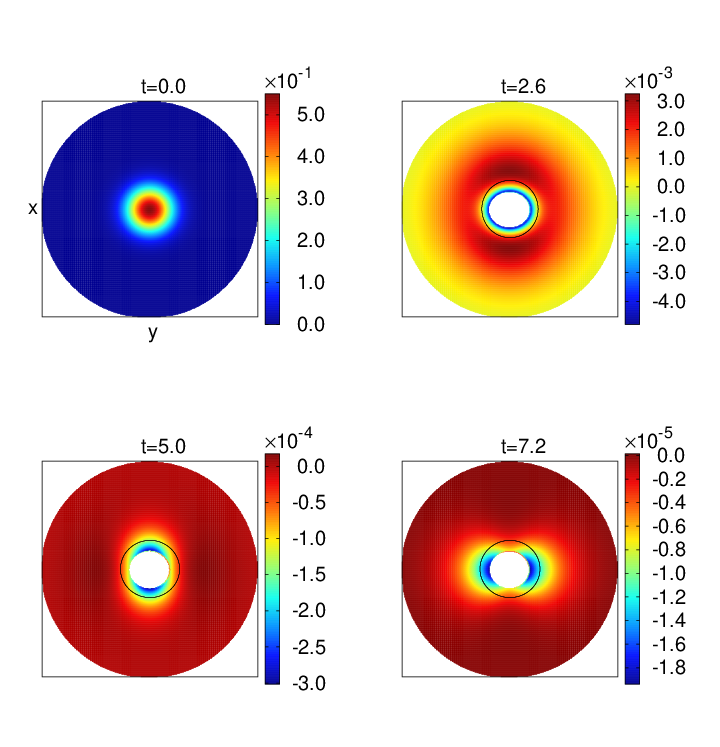
\includegraphics[width=5.2in,clip=true]{plots/bulkplots/L3/phi1/phi1_L3_snapshots_2by2.png}
\parbox{5.0in}{\caption{Snapshots of the scalar field profile $\bar{\varphi}$ on the $z=0$ slice in $(x,y)$ coordinates. In each plot, the black square denotes the boundary of the numerical grid, i.e. $x=\pm 1$ and $y=\pm 1$. The external boundary of the coloured part is the AdS boundary $\rho=1$. The black ellipse is the elliptic approximation of the Apparent Horizon (AH) at each time step. The internal boundary of the coloured region is the excision surface: we excise points inside an ellipse whose semi-axes are the AH ellipse semi-axes reduced by a factor $1-ex_{rbuf}=0.65$. (Highest resolution, $N_x=N_y=N_z=325$)
        }\label{fig:snapshotsscalarfield}}
\end{figure}

Figure \ref{fig:snapshotsscalarfield} shows four representative times of the scalar field profile $\bar{\varphi}$ on the equatorial plane $z=0$ for the highest resolution grid with $N_x=N_y=N_z=325$ grid points along each cartesian direction. Notice that, in all of these, $\bar{\varphi}=0$ at the AdS boundary as required by the Dirichlet boundary condition. At $t=0$, the asymmetry of the initial Gaussian profile is too small to be visible. At the beginning of evolution, we see that the scalar field starts spreading towards the AdS boundary but, before reaching this, it is attracted towards the centre and forms an apparent horizon (AH).  This occurs at $t=0.331481$ in the highest resolution simulation.
The asymmetry on the $(x,y)$-plane is clearly visible at $t=2.6$, where the scalar field is stretched along the $x$-direction. The elongation changes its direction multiple times during the evolution, as shown in the next two plots: it is along the $y$-axis at $t=5.0$ and again along the $x$-axis at $t=7.2$. Furthermore, we see that the largest part of the scalar field progressively disappears from the exterior part of the spacetime by entering the apparent horizon, hence the amplitude of the scalar field decreases. At later times, $t\simeq 9$, the value of the scalar field becomes consistent with 0 up to solution error (estimated by comparing $\bar{\varphi}$ at different resolutions) and the spacetime settles down to a Schwarzschild-AdS black hole.

\begin{figure}[!h]
        \centering
        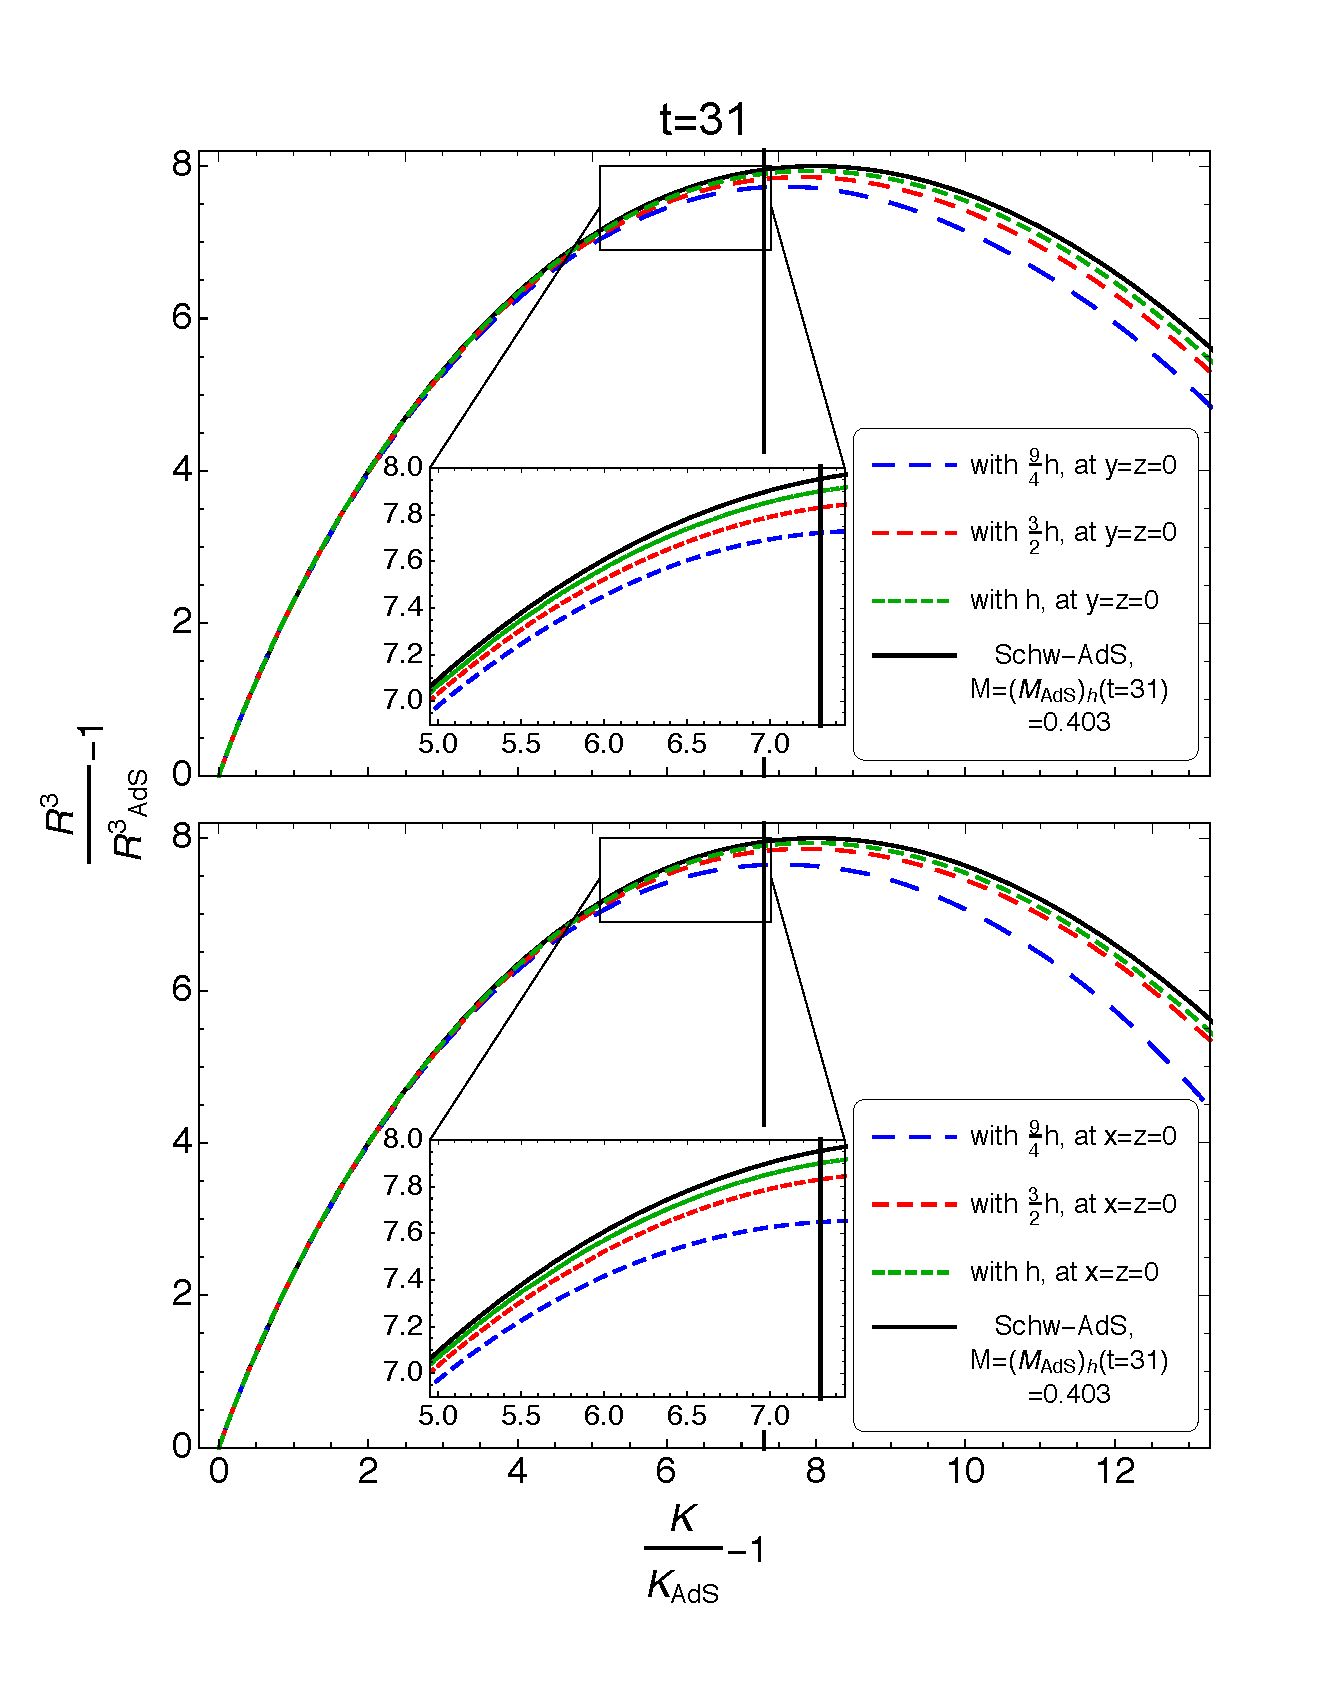
\includegraphics[width=5.25in,clip=true]{plots/bulkplots/compare_res/relriemanncube-relkretsch/combined_withzoom_fullplotrelRieCubeofrelkretschallres.pdf}
\parbox{5.0in}{\caption{Riemann cube scalar relative to $AdS_4$, $\frac{R^3}{R^3_{AdS}}-1$, as a function of Kretschmann scalar relative to $AdS_4$, $\frac{K}{K_{AdS}}-1$, for different resolutions at the last time step of the simulations, $t=31$, compared with the Schwarzschild-AdS case with mass given by $(M_{AdS})_h(t=31)=0.403$, i.e. the value of $M_{AdS}$ (see eq. \eqref{eq:AdSmasscalc}) for the resolution with grid spacing $h$ at time $t=31$. The black vertical line denotes the value of $\frac{K}{K_{AdS}}-1$ at the horizon of Schwarzschild-AdS. Relative Kretschmann increases as we move closer to the centre of the spacetime. Top panel: numerical curves are obtained from grid points on the $x$ axis (i.e. $y=z=0$). Bottom panel: numerical curves are obtained from grid points on the $y$ axis (i.e. $x=z=0$).
        }\label{fig:relRiemanncube-relKretschmann-comparison-SchwAdS}}
\end{figure}

%\begin{figure}[!h]
%        \centering
%        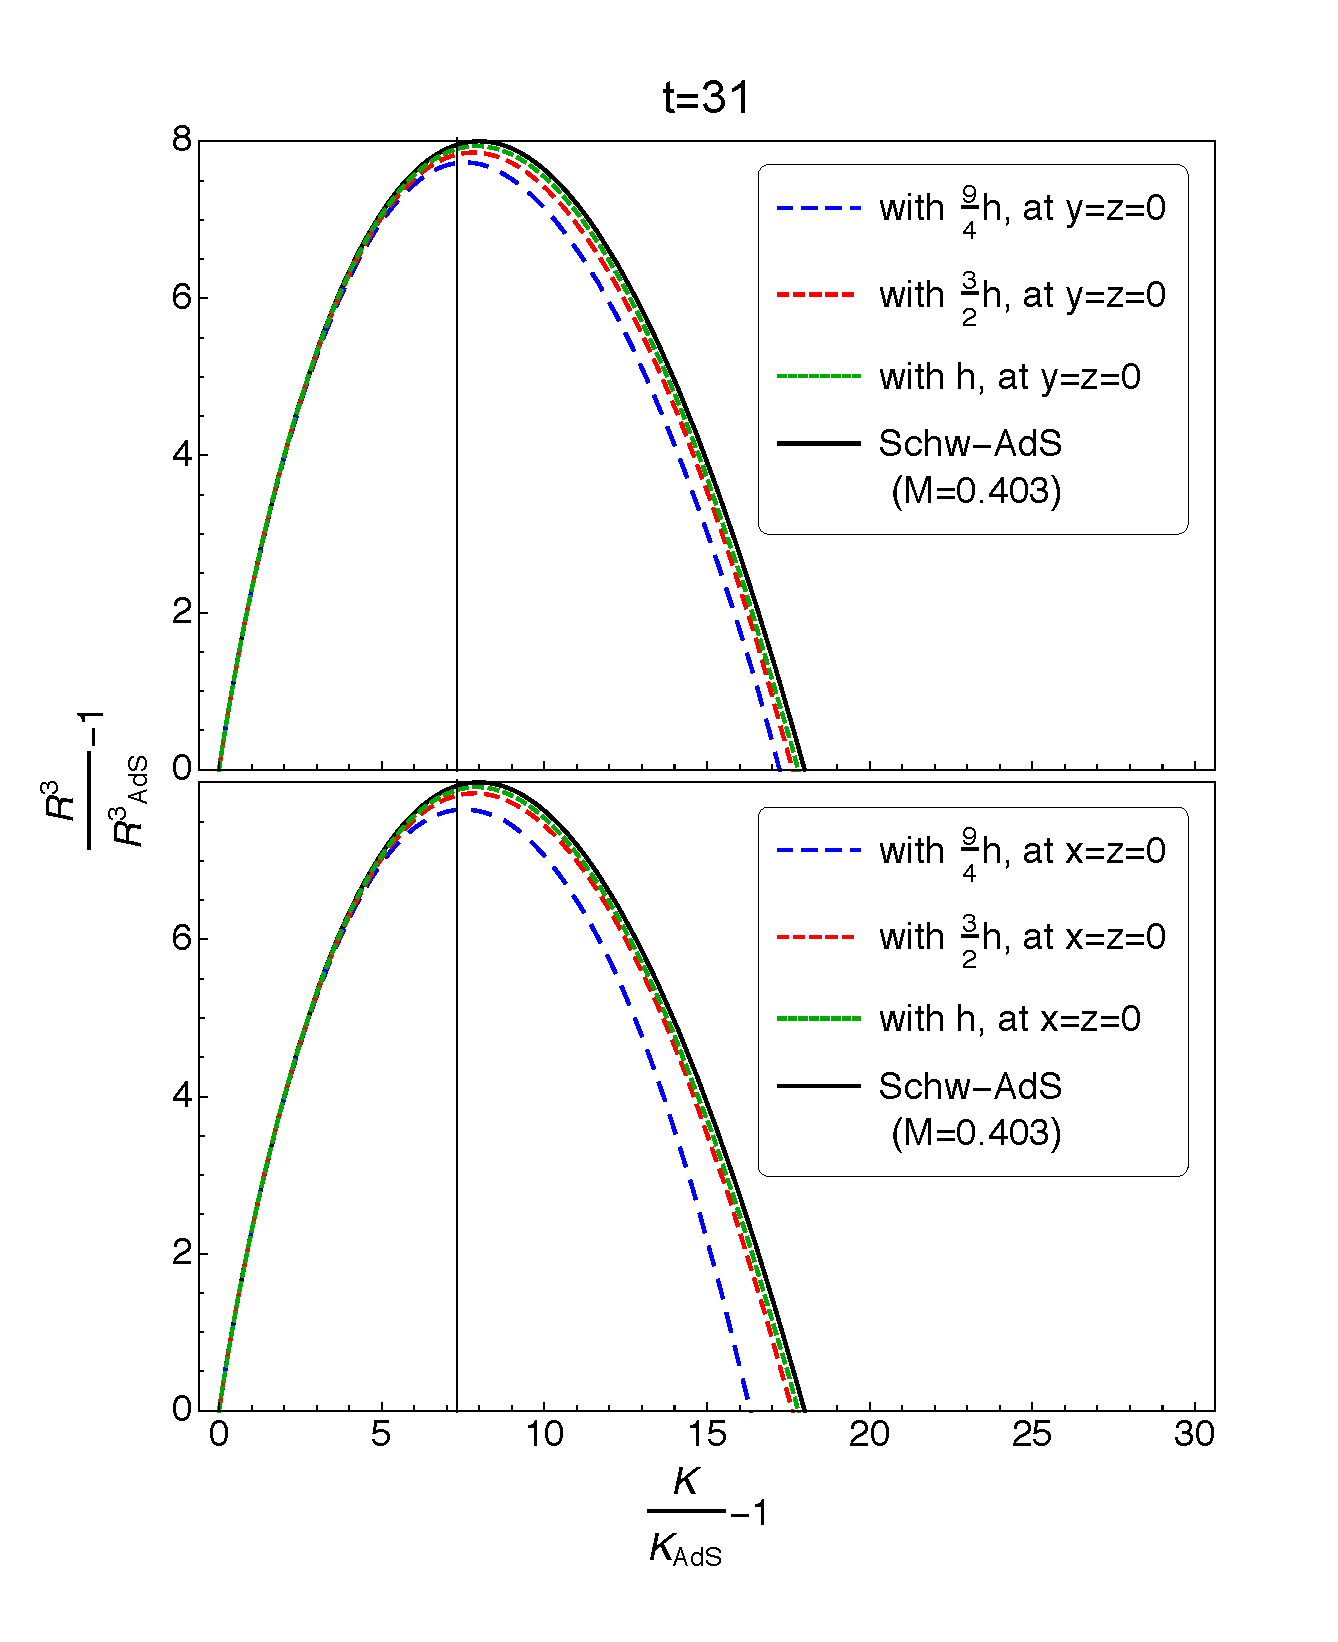
\includegraphics[width=5.0in,clip=true]{plots/bulkplots/compare_res/relriemanncube-relkretsch/option2_combinedplotrelRieCubeofrelkretschallres.pdf}
%\parbox{5.0in}{\caption{Riemann cube scalar relative to $AdS_4$, $\frac{R^3}{R^3_{AdS}}-1$, as a function of Kretschmann scalar relative to $AdS_4$, $\frac{K}{K_{AdS}}-1$, for different resolutions at the last time step of the simulations, $t=31$, compared with the Schwarzschild-AdS case with mass given by the value of $M_{AdS}$ at that time. Top panel: plot obtained using values on the $x$ axis (i.e. $y=z=0$). Bottom panel: plot obtained using values on the $y$ axis (i.e. $x=z=0$).
%        }\label{fig:relRiemanncube-relKretschmann-comparison-SchwAdS}}
%\end{figure}

\iffalse
\begin{figure*}
 \centering
\begin{multicols}{2}
    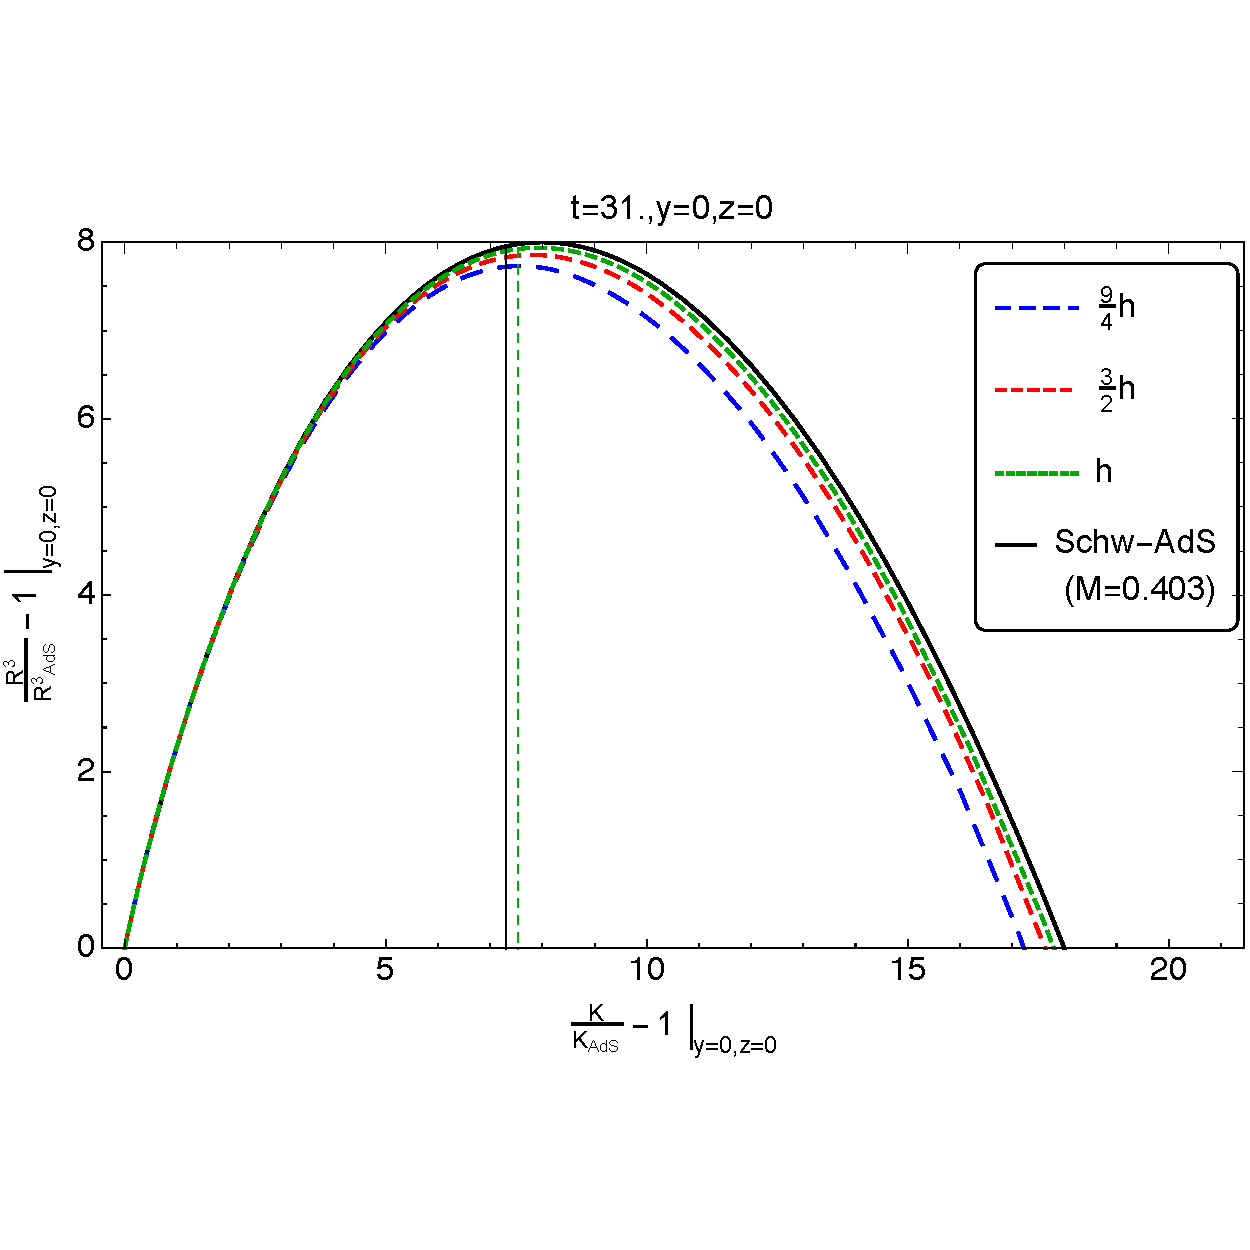
\includegraphics[width=3.1in,clip=true]{plots/bulkplots/compare_res/relriemanncube-relkretsch/y00_z00_plotalongxrelRieCubeofrelkretschallres.pdf}\par 
    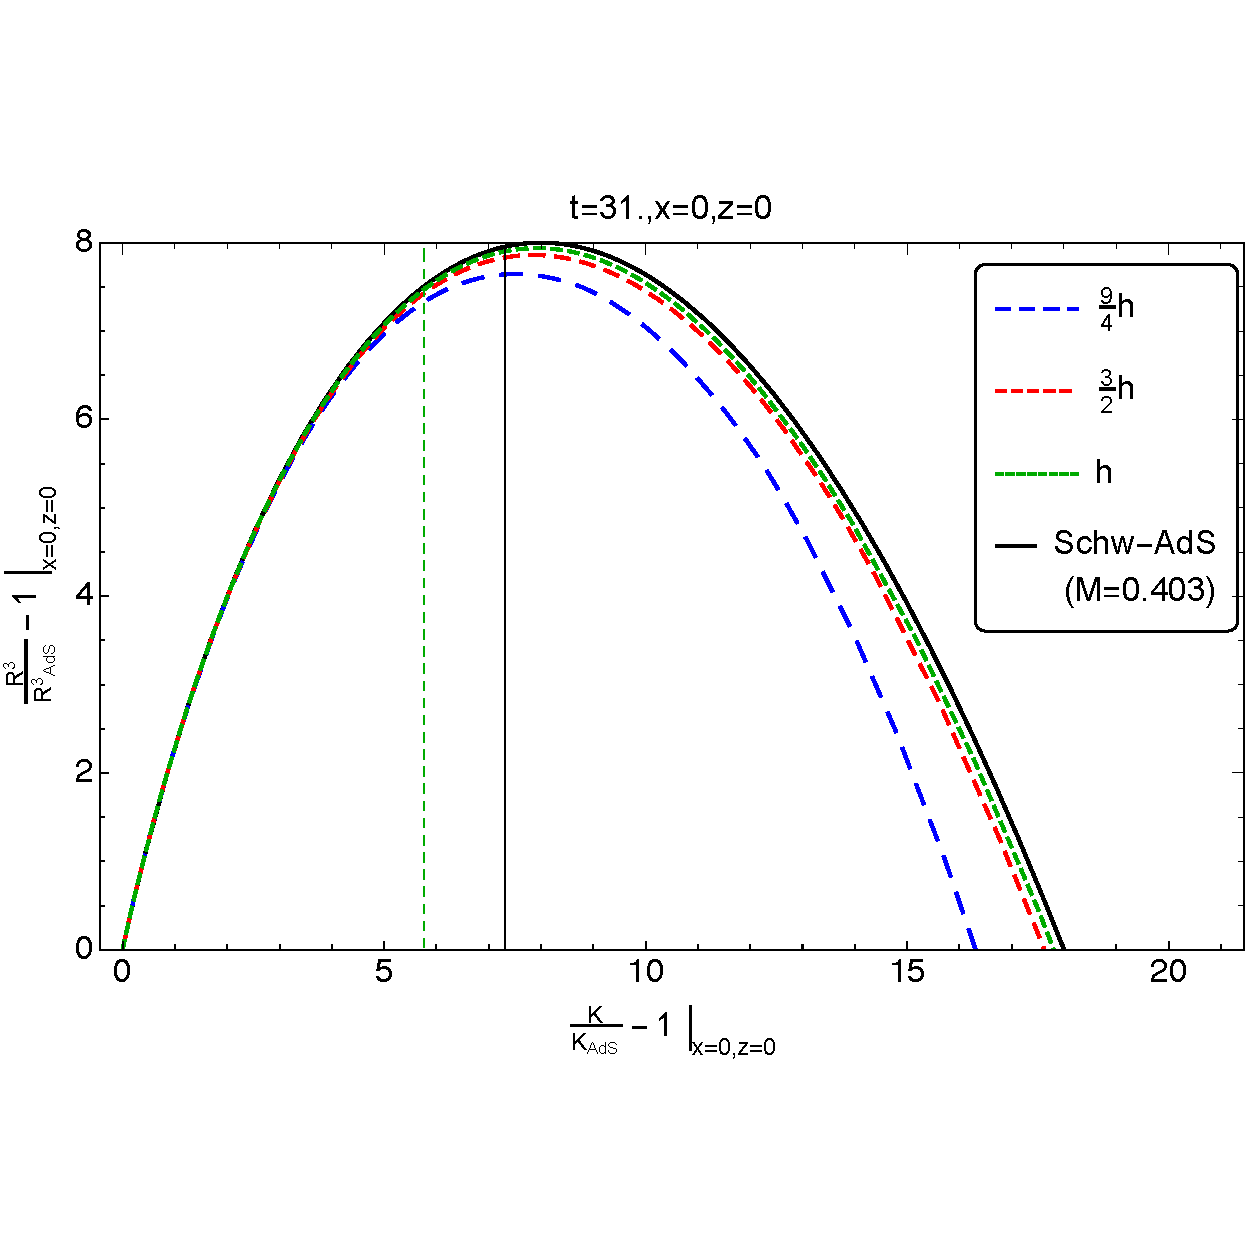
\includegraphics[width=3.1in,clip=true]{plots/bulkplots/compare_res/relriemanncube-relkretsch/x00_z00_plotalongyrelRieCubeofrelkretschallres.pdf}\par 
    \end{multicols}
\parbox{5.0in}{\caption{caption here}}
\end{figure*}
\fi

\iffalse
\begin{figure}
  \centering
  \subfloat{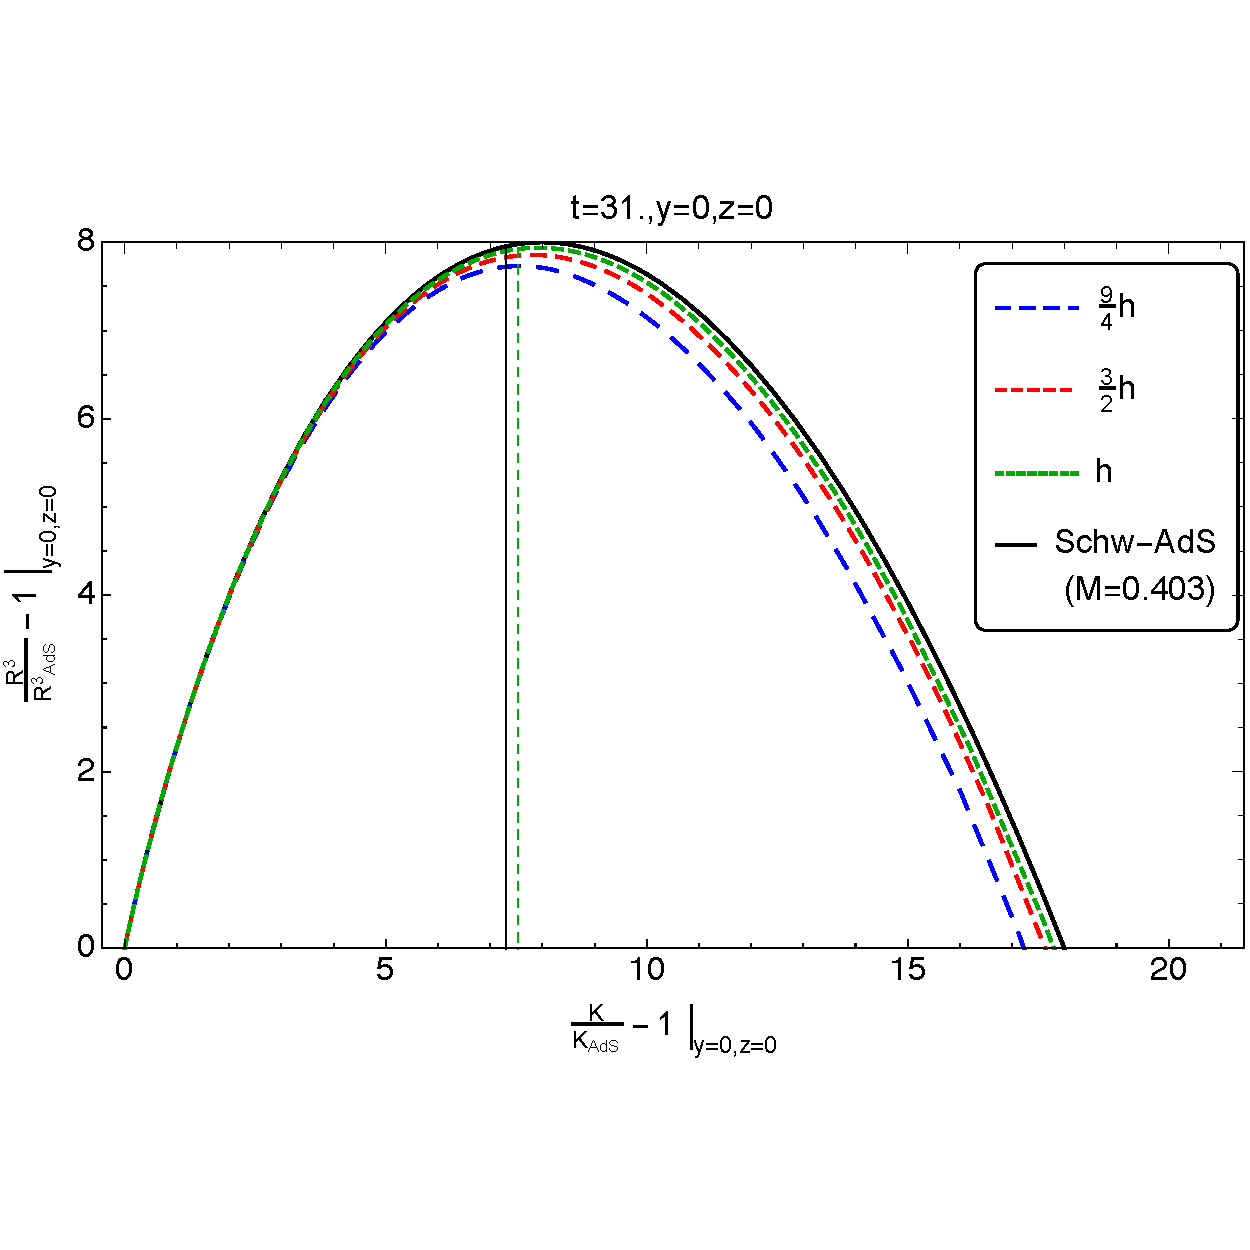
\includegraphics[width=4.0in,clip=true]{plots/bulkplots/compare_res/relriemanncube-relkretsch/y00_z00_plotalongxrelRieCubeofrelkretschallres.pdf} \label{fig:a}} \\
  \subfloat{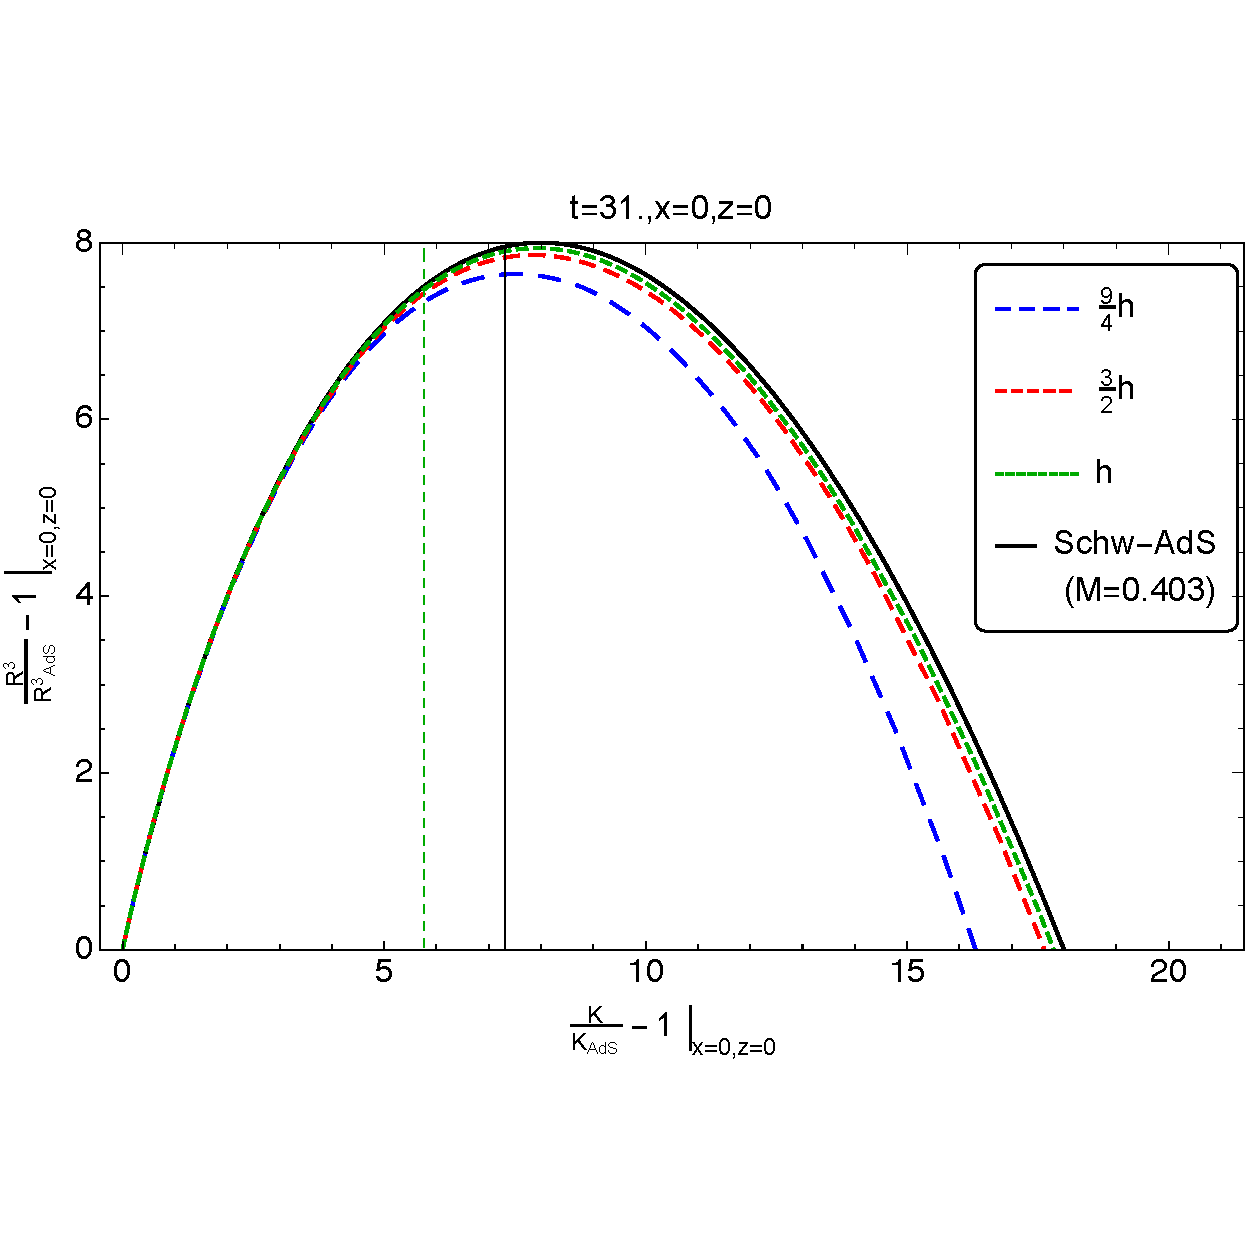
\includegraphics[width=4.0in,clip=true]{plots/bulkplots/compare_res/relriemanncube-relkretsch/x00_z00_plotalongyrelRieCubeofrelkretschallres.pdf} \label{fig:b}}
  \caption{a + b} \label{fig:AB}
\end{figure}
\fi

This can be seen in Figure \ref{fig:relRiemanncube-relKretschmann-comparison-SchwAdS}, in which we compare the numerical solution at the end of our simulations, $t=31$, to the Schwarzschild-AdS metric with mass $(M_{AdS})_h(t=31)=0.403$, namely the highest resolution value of $M_{AdS}$ (given by equation \eqref{eq:AdSmasscalc}) at $t=31$, as follows. We compute the Riemann cube scalar $R^3=R_{\mu\nu\rho\sigma}R^{\rho\sigma\gamma\delta}R_{\gamma\delta}^{\;\;\;\;\mu\nu}$, the Kretschmann scalar $K=R_{\mu\nu\rho\sigma}R^{\mu\nu\rho\sigma}$ and their corresponding values for pure $AdS_4$, $R^3_{AdS}$ and $K_{AdS}$, in order to show the relative Riemann scalar $\frac{R^3}{R^3_{AdS}}-1$ as a function of the Kretschmann scalar $\frac{K}{K_{AdS}}-1$ for the Schwarzschild-AdS spacetime (black line). We do the same for the numerical solution for different resolutions at grid points along the $x$ axis (i.e. at $y=z=0$, coloured lines of top panel) and the $y$ axis (i.e. at $x=z=0$, coloured lines of bottom panel). The black vertical line denotes the value of $\frac{K}{K_{AdS}}-1$ at the horizon of Schwarzschild-AdS. Notice that $\frac{K}{K_{AdS}}-1=0$ at the AdS boundary by construction, so going to larger values of $\frac{K}{K_{AdS}}-1$ is equivalent to moving towards the centre of the grid, therefore the vertical lines give an indication of the position of the AH relative to the AdS boundary.
The two plots indicate that, sufficiently close to the AdS boundary, the curvature of the numerical solution is almost identical to Schwarzschild-AdS. For clarity, this is shown using only values of the Riemann cube and Kretschmann scalars along the $x$ and $y$ axes, but we verified it for values from the entire grid. The numerical curvature starts to differ from the Schwarzschild-AdS profile as we get close to the AH (and it diverges strongly at values of $\frac{K}{K_{AdS}}-1$ corresponding to positions very close to the excision surface, as expected but not shown in the figure). However, the higher the resolution the closer we get to Schwarzschild-AdS even inside the AH.
Finally, we notice that for low resolutions a persistent asymmetry between the $x$ and $y$ axes is visible also at late times both outside and inside the horizon, but this disappears for high enough resolutions.


\subsection{Boundary scalar field and stress-energy tensor}
\label{sec:resbouset}

In this section we consider the evolution of quantities on the boundary $S^2$ at $\rho=1$, defined in Section~\ref{sec:bouset2}. They are obtained via third order extrapolation from bulk points, with the only exception of the $t=0$ plot of Figure \ref{fig:snapshotsbdyphi}: this is computed analytically from the initial distorted Gaussian profile \eqref{eq:scaGaupro}, as extrapolation would give values smaller than the solution error of the function. 

\begin{figure}[!h]
        \centering
        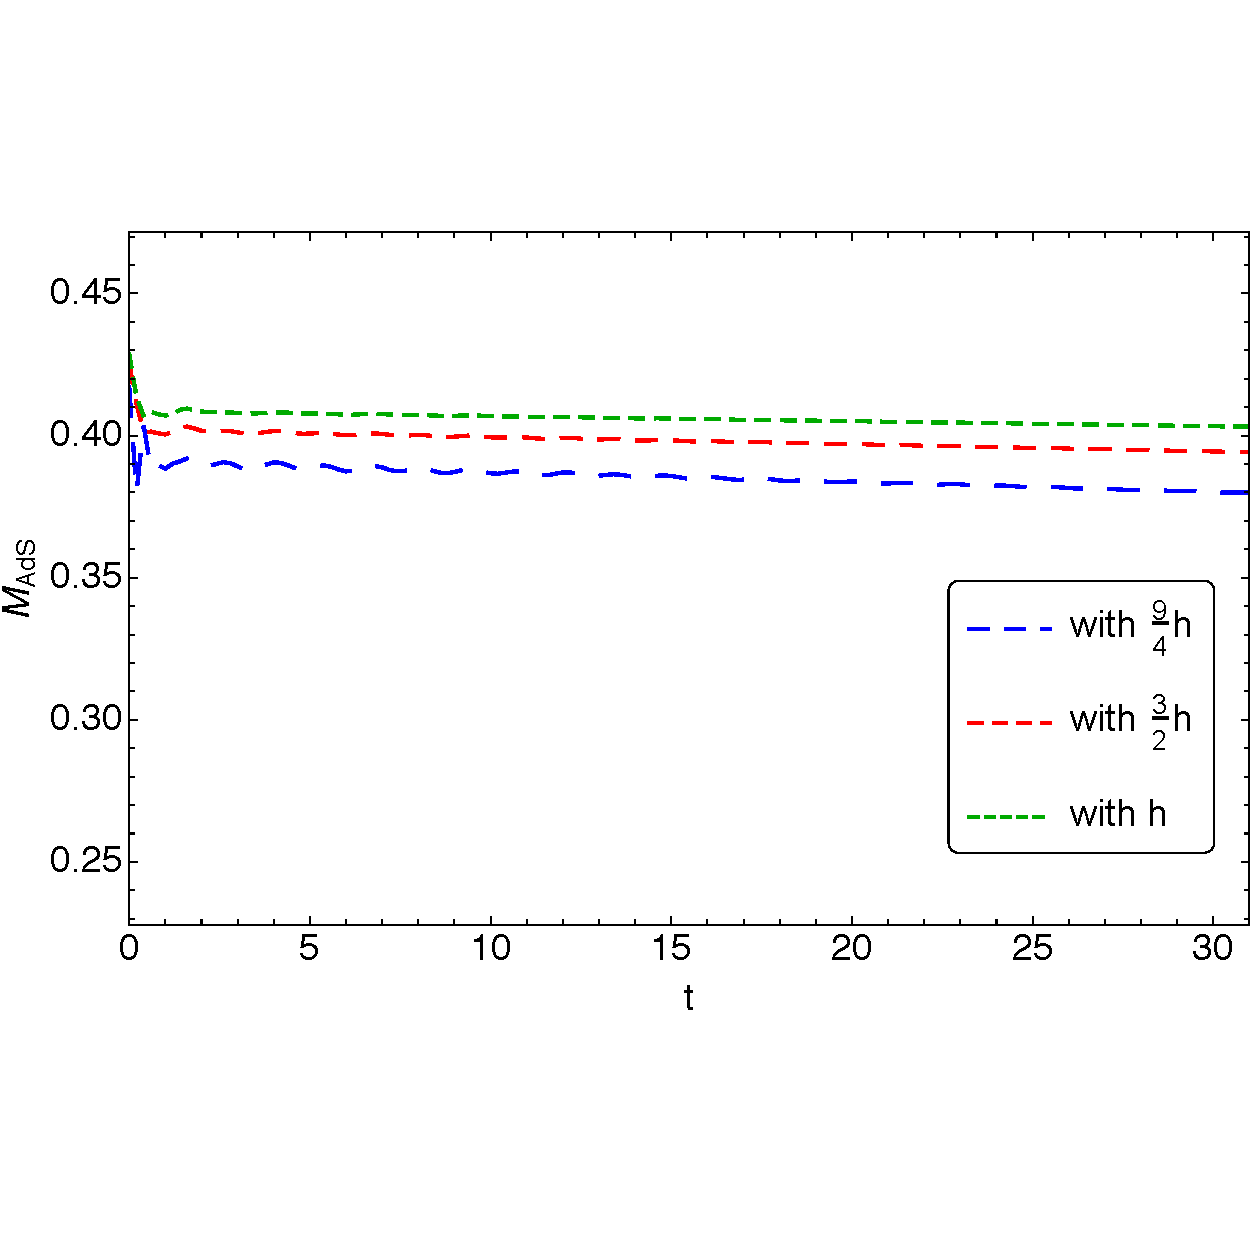
\includegraphics[width=4.5in,clip=true]{plots/timeseries/AdSmass/fullplotfillregtAdSmassallres.pdf}
\parbox{5.0in}{\caption{Time evolution of AdS mass for different resolutions.
        }\label{fig:AdSmass-crop}}
\end{figure}

We start by looking at the values of the AdS mass, given by \eqref{eq:AdSmasscalc}, with respect to $t$ for different resolutions in Figure \ref{fig:AdSmass-crop}, which shows that the Schwarzschild-AdS spacetime that our deformed black hole settles down to has a mass of around $0.4$ in units of the AdS length scale. In this plot we also notice an unphysical mass loss for low resolutions, although $M_{AdS}$ converges to a constant in time as resolution increases, as desired. In particular, data displays first order convergence instead of the second order of boundary data, inherited from bulk convergence. We believe that this can be understood as follows. As explained in Appendix~\ref{sec:extrapconvbdy}, we can only expect to see second order convergence at the boundary if we consider values extrapolated via the scheme satisfying the common points criterion (see point 1. of Appendix~\ref{sec:extrapconvbdy}) restricted to the convergent range given at point 2. of Appendix~\ref{sec:extrapconvbdy}. However, once convergence has been verified, we use more accurate data obtained via a scheme that no longer requires 1., but it allows the use of any point in the range given at 2.. As a consequence, we can no longer predict second order for this data. In fact, even if we considered data for the AdS mass density extrapolated from common points, we would have a similar issue in Figure \ref{fig:AdSmass-crop} due to the method used to approximate the integral of equation \eqref{eq:AdSmasscalc} through the Wolfram Mathematica software. More precisely, before numerically integrating (via the NIntegrate command with default GlobalAdaptive method), the values for the AdS mass density at boundary points are interpolated (with first order interpolation, as this is the only one allowed by the Interpolation command for unstructured grids, such as the ones we have at the boundary) to obtain an integrand function defined over the entire boundary $S^2$. This interpolation does not use points common to all resolutions, hence the argument at point 1. of Appendix~\ref{sec:extrapconvbdy} (this time applied to interpolation) tells us again that we cannot expect second order convergence. Despite these complications, as we increase the bulk grid refinement, all these approximations become more and more accurate and we expect to get closer to the true value of the boundary function. In other words, we expect some order of convergence at each boundary point. Therefore, it is not surprising that Figure \ref{fig:AdSmass-crop} shows the lowest possible convergence order, i.e. the first one.

%We believe this is due to the method used to approximate the integral of equation \eqref{eq:AdSmasscalc} through the Wofram Mathematica software. Before numerically integrating (via the NIntegrate command with default GlobalAdaptive method), the values for the AdS mass density at boundary points are interpolated to obtain a function defined over the entire boundary $S^2$ (via the Interpolation command). This interpolation can only be performed at first order for data on an unstructured grid, such as the one we have at the boundary.

\begin{figure}[!h]
        \centering
        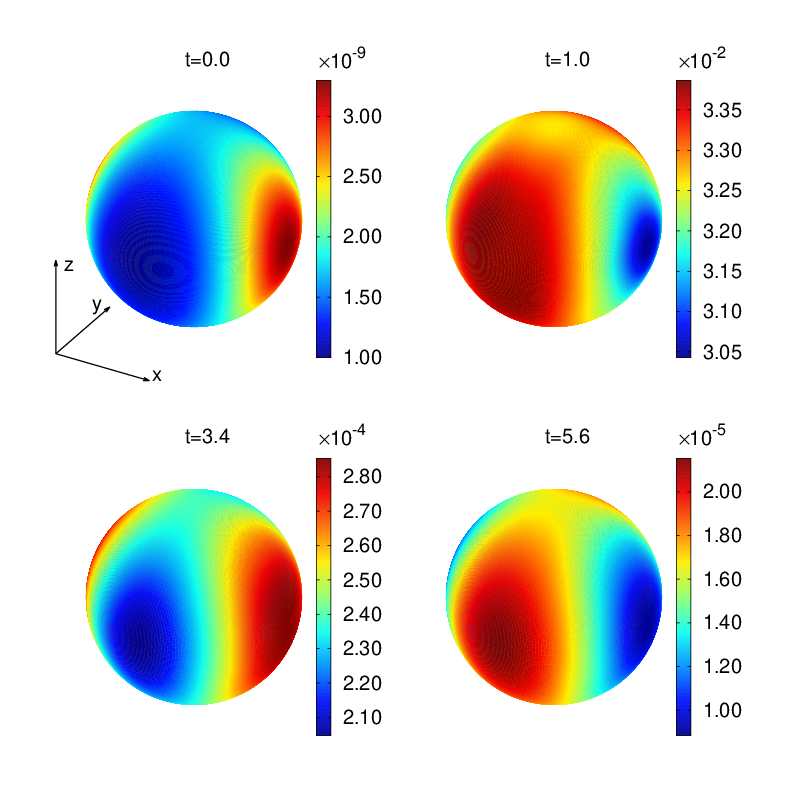
\includegraphics[width=5.0in,clip=true]{plots/bdyplots/L3/bdyphi/sphereplots_bdyphi_L3_2by2.png}
\parbox{5.0in}{\caption{Snapshots of the scalar field of the boundary CFT, $\langle \bar{\varphi}\rangle_{CFT}$. The first snapshot is obtained analytically from the initial scalar field profile. The remaining three are obtained by third order extrapolation and subsequent smoothening via a low-pass filter with threshold frequency $\omega=0.5$. (Highest resolution, $N_x=N_y=N_z=325$)
        }\label{fig:snapshotsbdyphi}}
\end{figure}

Figure \ref{fig:snapshotsbdyphi} shows four snapshots of the scalar field of the boundary CFT, $\langle \bar{\varphi}\rangle_{CFT}$.
Unlike the $z=0$ slice snapshots of Figure \ref{fig:snapshotsscalarfield}, these sphere plots show the asymmetry in all three Cartesian direction. In fact, the asymmetry of the initial data is already visible at $t=0$, where the different values of eccentricities along the three Cartesian direction (largest along $x$ and smallest along $y$) are evident in this plot. At this time, the boundary scalar field is overall very small, which is expected since the initial $\bar{\varphi}$, given by \eqref{eq:scaGaupro}, is localised near $\rho=0$.
As noticed in Figure \ref{fig:snapshotsscalarfield}, the asymmetry changes direction during evolution, but interestingly it is always strongest along $x$ and weakest along $y$ or viceversa. Furthermore, a direct comparison with Figure \ref{fig:snapshotsscalarfield} shows that the features present at a certain $t$ at the boundary take approximately $\pi/2\simeq1.6$ to reach the interior of the bulk, i.e. about half light-crossing time, as expected. At later times, similarly to the bulk, the scalar field at the boundary becomes negligible as the spacetime settles down to Schwarzschild-AdS.

\begin{figure}[!h]
        \centering
        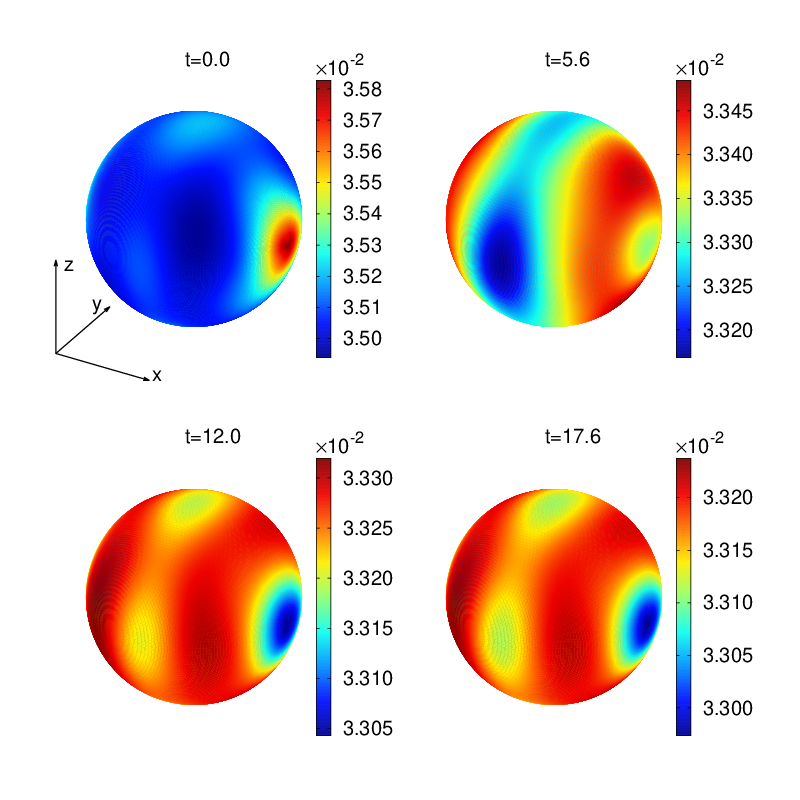
\includegraphics[width=5.0in,clip=true]{plots/bdyplots/L3/bdyenergydensity/sphereplots_bdyenergydensity_L3_2by2.png}
\parbox{5.0in}{\caption{Snapshots of energy density $\langle\epsilon\rangle_{CFT}$ at the boundary, obtained by third order extrapolation and smoothened via a low-pass filter with threshold frequency $\omega=0.25$. The scale of each snapshot has fixed interval length centred at the mean value of  $\langle\epsilon\rangle_{CFT}$ at the corresponding evolution time to make the approach to a uniform configuration more visible. (Highest resolution, $N_x=N_y=N_z=325$)
        }\label{fig:snapshotsenergydensity}}
\end{figure}

Figure \ref{fig:snapshotsenergydensity} displays the energy density of the boundary CFT, $\langle\epsilon\rangle_{CFT}$. At $t=0$ this is strongly asymmetric along the $x$-direction, as expected from the shape of the initial scalar field \eqref{eq:scaGaupro}. After then, $\langle\epsilon\rangle_{CFT}$ undergoes a phase of strong evolution with several changes of elongation direction, sampled at $t=5.6$ and terminating at approximately $t=7.2$. From that time onwards, $\langle\epsilon\rangle_{CFT}$ settles down to a uniform configuration, as appropriate for the Schwarzschild-AdS case. Approach to uniformity is emphasized by using colour scales with fixed interval length, centred at the mean value of $\langle\epsilon\rangle_{CFT}$ at the corresponding evolution time.

%After then, $\epsilon_{CFT}$ shows non-trivial evolution up and, again, changes of elongation axisuntil approximately $t=11.0$, before settling down. In fact, in an interval of time $\Delta t=5.6$, $\epsilon_{CFT}$ changes significantly at the beginning (again exhibiting changes of elongation axis) but it stays essentially unchanged from $t=12$. The small drop of $\epsilon_{CFT}$ shown at $t=17.6$ is consistent with the small loss of mass noticed in Figure \ref{fig:AdSmass-crop}

%Figure \ref{fig:snapshotsenergydensityrelativetoSchw} displays the energy density of the boundary CFT relative to the Schwarzschild-AdS value, i.e. $\frac{\epsilon_{CFT}}{\epsilon_{CFT (S-AdS)}}-1$ where $\epsilon_{CFT (S-AdS)}=\frac{M}{4\pi}$ and for $M$ we use the AdS mass $M=0.410594$ of the last time shown, $t=5.6$. This quantity is initially significantly different from $\epsilon_{CFT (S-AdS)}$ but it quickly approaches its Schwarzschild-AdS analog and it remains essentially unchanged from $t=3.4$ onwards.

%\begin{figure}[h]
 %       \centering
 %       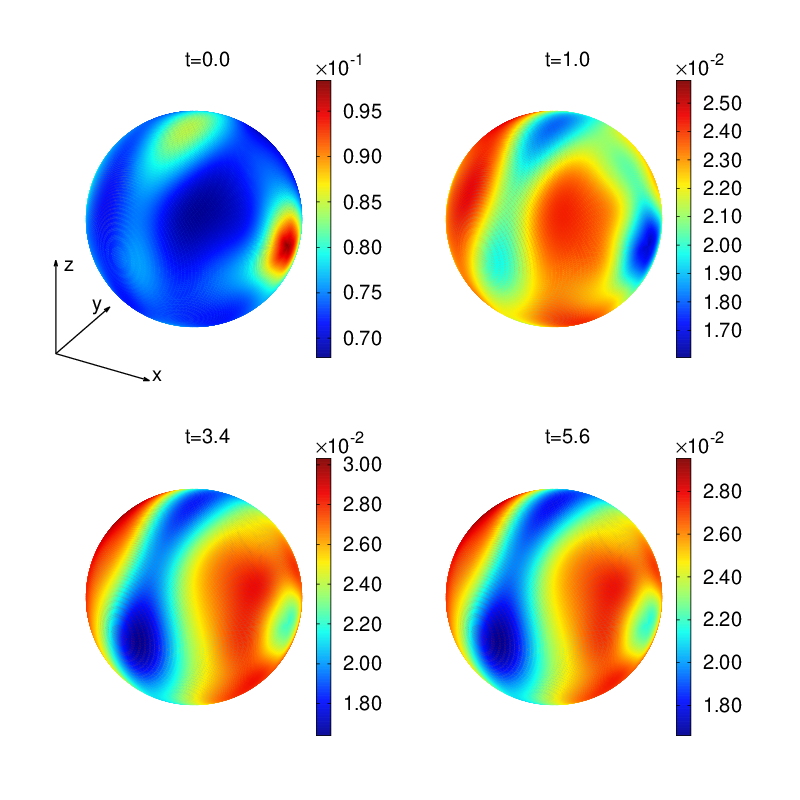
\includegraphics[width=5.0in,clip=true]{plots/bdyplots/L3p5/bdyenergydensityrelativetoschw/sphereplots_bdyenergydensityrelativetoschw_L3p5_2by2.png}
%\parbox{5.0in}{\caption{Snapshots of energy density relative to Schwarschild-AdS with the AdS mass of t=5.6, $M=0.410594$ i.e. $\frac{\epsilon_{CFT}}{\epsilon_{CFT (S-AdS)}}-1$, at the boundary (L3p5 resolution, $N_x=487$).
%        }\label{fig:snapshotsenergydensityrelativetoSchw}}
%\end{figure}

%Figure \ref{fig:snapshotsbdyanisotropy} displays the anisotropy of the boundary CFT $\Delta p_{CFT}$. This is at all times consistent with the vanishing value of the Schwarzschild-AdS case.


%\begin{figure}[h]
%        \centering
%        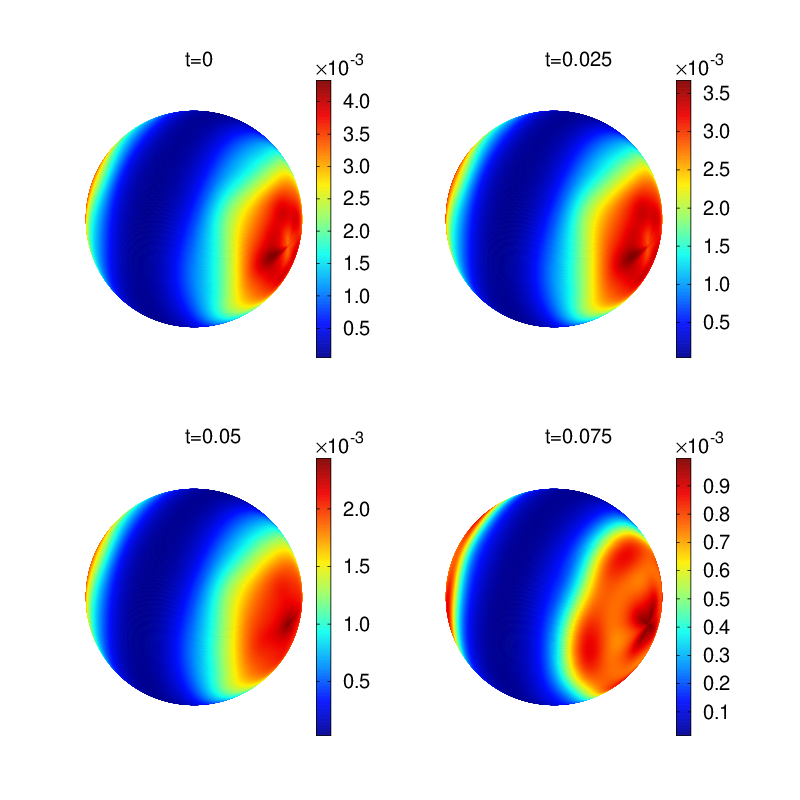
\includegraphics[width=5.0in,clip=true]{plots/bdyplots/L3/bdyanisotropy/sphereplots_bdyanisotropy_L3_2by2.png}
%\parbox{5.0in}{\caption{Snapshots of anisotropy at the boundary (L3 resolution, $N_x=325$).
%        }\label{fig:snapshotsbdyanisotropy}}
%\end{figure}

\begin{figure}[!h]
        \centering
        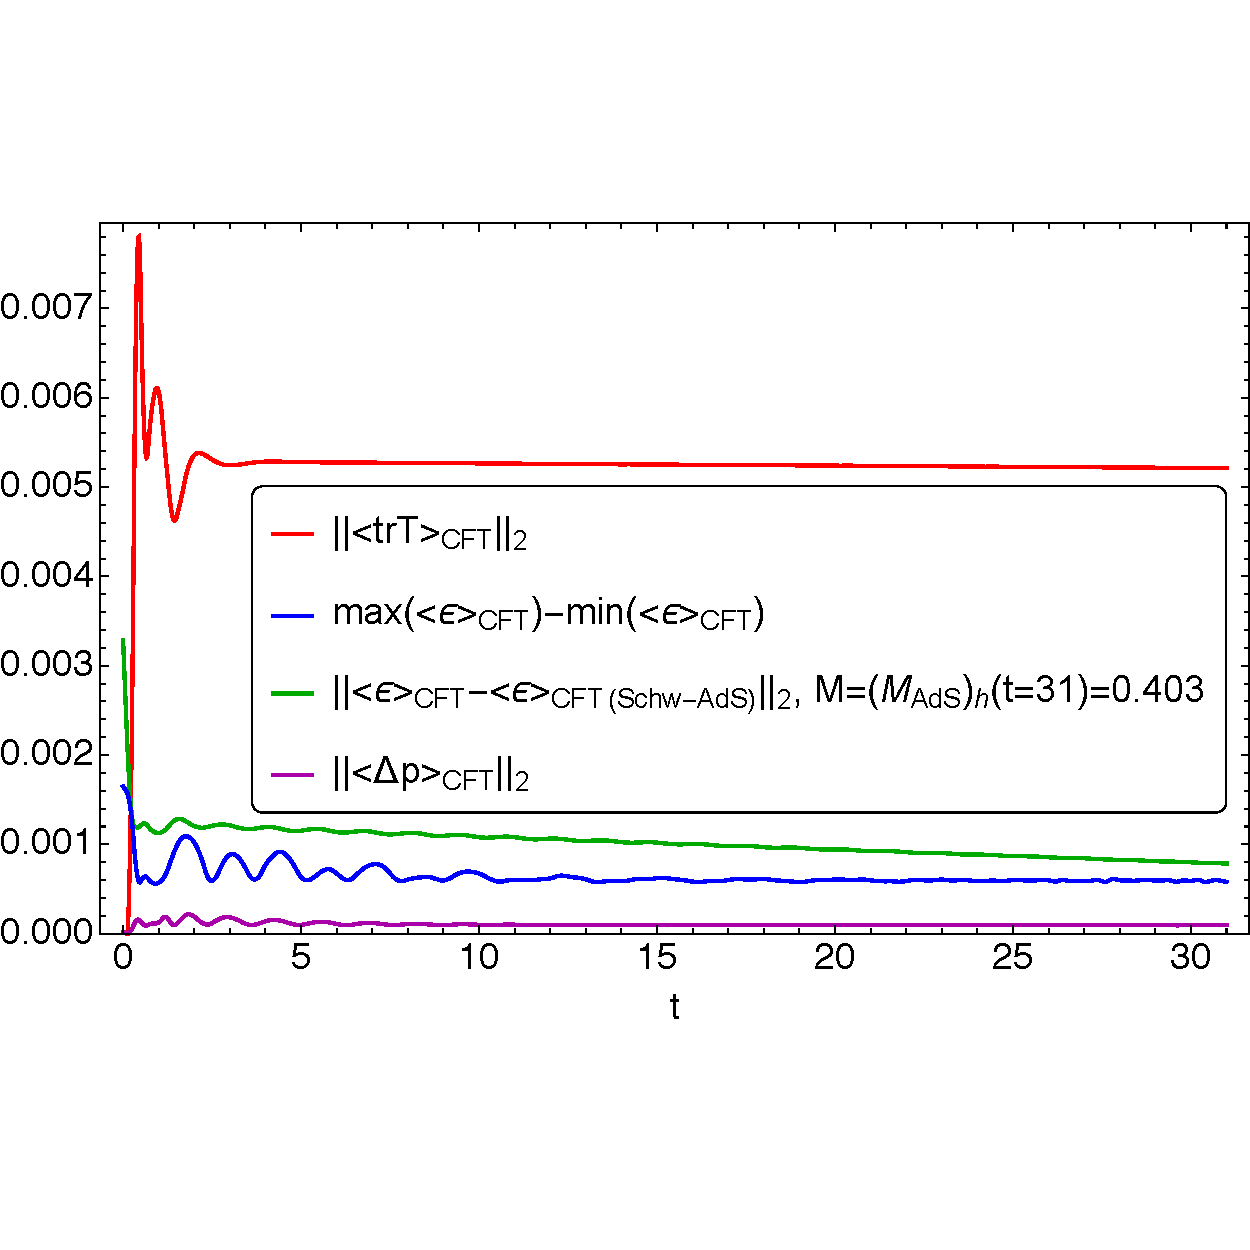
\includegraphics[width=5.0in,clip=true]{plots/timeseries/L2-norm_trace_anisotropy_energydensityminusschw_maxminusminenergydensity/fullplotfillregttraceanisotropyenergydensityminusschwmaxminusminbdyenergydensity_L3.pdf}
\parbox{5.0in}{\caption{Comparison of boundary quantities with error estimate given by the deviation of the $L^2$-norm of $\langle trT\rangle_{CFT}$ from its predicted zero value for the 2+1 boundary CFT (red line). We consider the following boundary quantities: difference between maximum and minimum of boundary energy density $\langle\epsilon\rangle_{CFT}$ (blue line), $L^2$-norm of difference between $\langle\epsilon\rangle_{CFT}$ and the Schwarzschild-AdS value $\langle\epsilon\rangle_{CFT(Schw-AdS)}=\frac{M}{4\pi}$ (green line), with Schwarzschild mass $M=(M_{AdS})_h(t=31)=0.403$ (i.e. the value of $M_{AdS}$ for the resolution with grid spacing $h$ at time $t=31$), $L^2$-norm of boundary anistropy $\langle\Delta p\rangle_{CFT}$ (magenta line). Plot obtained from the data of the highest resolution run ($N_x=N_y=N_z=325$), but at any resolution these quantities exhibit the same hierarchy, although at different scales. Boundary quantities are computed by third order extrapolation.
        }\label{fig:fullplotfillregttraceanisotropyenergydensityminusschwmaxminusminbdyenergydensity.pdf}}
\end{figure}

More information about the energy density at the boundary can be deduced from Figure \ref{fig:fullplotfillregttraceanisotropyenergydensityminusschwmaxminusminbdyenergydensity.pdf}. Given that $\langle trT\rangle_{CFT}$ vanishes for a conformal field theory in 2 spatial and 1 time dimensions, such as the one at the AdS boundary, the $L^2$-norm of the numerical values of $\langle trT\rangle_{CFT}$ (red line) is used as an error estimate for boundary quantities. We compare this error with the difference between maximum and minimum of $\epsilon_{CFT}$ (blue line), the $L^2$ norm of the difference between $\langle\epsilon\rangle_{CFT}$ and its Schwarzschild-AdS value $\langle\epsilon\rangle_{CFT(Schw-AdS)}=\frac{M}{4\pi}$ (green line), with $M=(M_{AdS})_h(t=31)=0.403$ (i.e. the highest resolution value of $M_{AdS}$ at $t=31$ as given by \eqref{eq:AdSmasscalc}), and the $L^2$ norm of $\langle\Delta p\rangle_{CFT}$ (magenta line). We compute these quantities from the data of the highest resolution simulation (i.e. $N_x=N_y=N_z=325$), but at any resolution the hierarchy is the same, although it appears at different scales.
If we exclude very early times, we see that (i) $\max(\langle\epsilon\rangle_{CFT})-\min(\langle\epsilon\rangle_{CFT})$ is consistent with 0, which confirms that the energy density becomes uniform in time; (ii) $||\langle\epsilon\rangle_{CFT}-\langle\epsilon\rangle_{CFT(Schw-AdS)}||_2$ is consistent with 0 and decreasing in time, which shows that the energy density settles down to $\langle\epsilon\rangle_{CFT(Schw-AdS)}$, as expected, (iii) $||\langle\Delta p\rangle_{CFT}||_2$ is consistent with 0, as appropriate for the boundary anistropy of Schwarzschild-AdS.

%\begin{figure}%
%    \centering
%    \subfloat[x-dependency]{{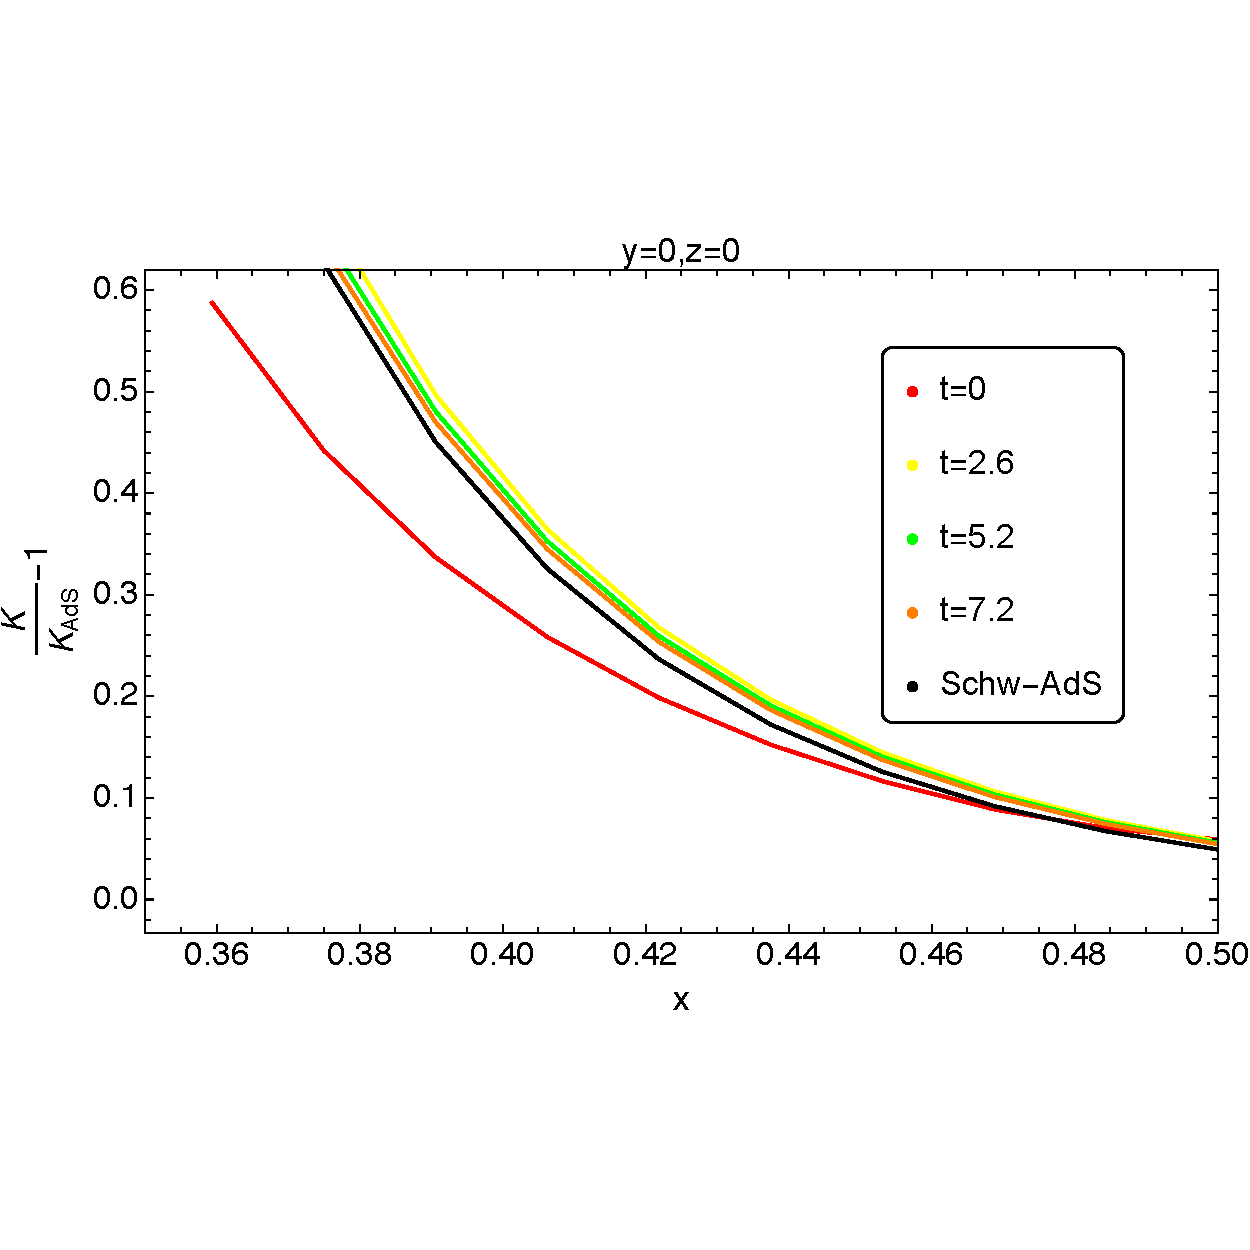
\includegraphics[width=3.0in]{plots/bulkplots/L2/relkretsch/fullplotxcoordrelkretschL2res-cropped.pdf} }}%
%    \qquad
%    \subfloat[y-dependency]{{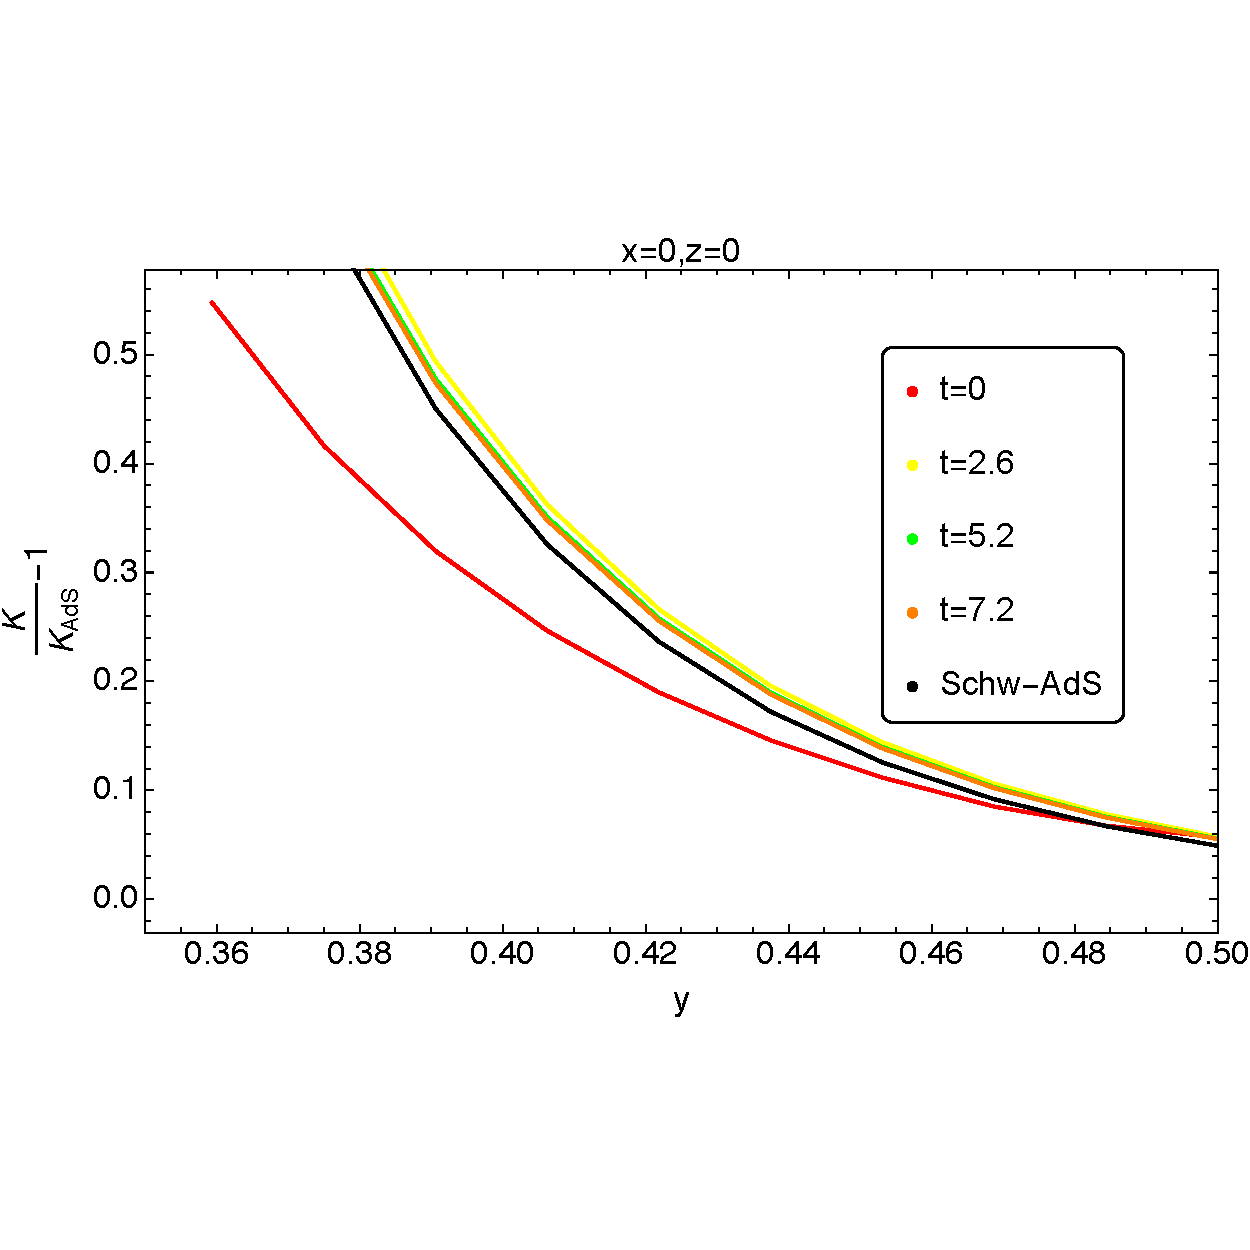
\includegraphics[width=3.0in]{plots/bulkplots/L2/relkretsch/fullplotycoordrelkretschL2res-cropped.pdf} }}%
%    \caption{Time evolution of Kretschmann: the Kretschmann scalar of the solution approaches the one for Schwarzschild-AdS}%
%    \label{fig:example}%
%\end{figure}




\section{Discussion}\label{sec:Discussion}

We have presented the first proof-of-principle Cauchy evolution of an asymptotically AdS spacetime determined by the Einstein-Klein-Gordon equations with no symmetry assumptions. Stability of the numerical code is achieved through the gauge choice \eqref{eqn:target_gauge_xyz},\eqref{eqn:target_gauge_t} near the AdS boundary. The reliability of the code has been tested and a brief analysis of the numerical solution for stationary initial data with completely asymmetric Gaussian massless scalar field has been provided.

We observe the collapse of the scalar field into a black hole and the ringdown to Schwarzschild-AdS, in both bulk and boundary quantities.
Deviations from Schwarzschild-AdS at late times are consistent with 0 within estimates of the numerical error, however the dominant spherical harmonic in the decomposition of the spatial profile of the scalar field in the bulk becomes higher and higher during the evolution. These non-spherically symmetric deviations might trigger a non-linear instability (unlike spherically symmetric deviations, under which Schwarzschild-AdS is stable [cite Holzegel, Smulevici]) that can only be revealed by evolving for longer times. More evidence could be found by decomposing the scalar field profile into spherical harmonics and showing that the radial part is non-vanishing near the boundary for a very long time. We leave this for future studies.

In this work we limited ourselves to $d=4$ spacetime dimensions, but the calculation outlined in Section~\ref{sec:gauge_choice} would be almost identical if we were to study 3+1 Cartesian evolution of asymptotically AdS spacetimes in any $d\geq4$ dimensions. In particular, the stable gauge found with this method would be the same up to a numerical factor. Even more interestingly, perhaps, a comparison between \eqref{eqn:target_gauge_xyz},\eqref{eqn:target_gauge_t} and the corresponding result in [cite arXiv:1706.04199 [hep-th] ] (see eq. (S10) ) clearly suggests a trend for the expression of the stable gauge in $D+1$ dimensions for any number $D\geq1$ of spatial dimensions. If this trend were confirmed, repeating the calculation above would not be necessary when changing the value of $D$. \textcolor{blue}{Furthermore, we see no obstacles in applying the scheme presented here to cases with different types of matter fields, different types of global coordinates, or even non-global Poincar\'{e} patches.}

We expect to be able to tackle several interesting problems in asymptotically AdS spacetimes using this code. The most direct application would be the study of gravitational collapse of a massless scalar field with zero angular momentum in $AdS_4$. This has been analyzed in spherical symmetry by [CITE Bizon-Rostworowski] and in axisymmetry by [Bantilan-Figueras-Kunesch], although the two studies probe different ranges for the amplitude of the scalar field, so a direct comparison cannot be made. Solving the evolution equations through our code, the details of the collapse could be analysed even further in full generality.

Other possible applications, requiring only minor additions to the capabilities of the current code, are the study of binary black hole mergers and black hole instabilities in AdS. In particular, the evolution of superradiantly unstable (see [cite Brito, Cardoso, Pani] for a review on superradiance) initial data for a Kerr-AdS black hole spacetime was followed in [cite CHESLER,LOWE], without imposing symmetries, up to approximately 290 light-crossing times using a characteristic scheme [cite Chesler, Yaffe]. This showed a transition of the Kerr-AdS black hole to a rotating black hole with one helical Killing field consistent with a black resonator [cite Dias, Santos, Way]. Since black resonators are fastly rotating black holes with an ergo-region, they are also unstable to superradiance [cite  Hawking, Reall] [cite Green, Hollands, Ishibashi, Wald] hence a cascade to smaller and smaller resonators, potentially leading to a violation of the weak cosmic censorship conjecture, was suggested [cite Niehoff,Santos,Way]. The authors of [cite CHESLER,LOWE] see a second transition at late times that could be the beginning of such cascade but they do not evolve further as Adaptive Mesh Refinement (AMR) becomes crucial to resolve small structures in a reasonable amount of running time. A code such as the one presented here, having AMR capabilities already built in, could be successful in reaching later stages of the evolution and potentially addressing the question about the end-state of superradiant instability of Kerr-AdS.



\section*{Acknowledgements}
HB and PF are supported by the European Research Council Grant No. ERC-2014-StG 639022-NewNGR. PF is also supported by a Royal Society University Research Fellowship (Grant No. UF140319 and URF\textbackslash R\textbackslash 201026) and by a Royal Society Enhancement Award (Grant No. RGF\textbackslash EA\textbackslash 180260).  LR is supported by a QMUL PhD scholarship. We acknowledge the use of Athena at HPC Midlands+, which was funded by the EPSRC on 
grant EP/P020232/1, in this research, as part of the HPC Midlands+ consortium. This research also utilised Queen Mary's Apocrita HPC facility, supported by QMUL Research-IT. http://doi.org/10.5281/zenodo.438045.

\appendix
\setcounter{tocdepth}{1}
\numberwithin{equation}{section}
\section{Generalized Harmonic Formulation}
\label{sec:GHfor}

The generalized harmonic formulation of the Einstein equations is based on coordinates $x^\alpha$ that each satisfies a wave equation $\Box x^{\alpha}=H^\alpha$ with source functions $H^\alpha$.
As long as the constraint $0=C^\alpha \equiv H^\alpha-\Box x^\alpha$ is satisfied, we can then write the trace-reversed Einstein equations in $d$ dimensions with cosmological constant $\Lambda$
\begin{equation}
0=R_{\alpha\beta} - \frac{2\Lambda}{d-2} g_{\alpha\beta} - 8\pi\left( T_{\alpha\beta} - \frac{1}{d-2} {T^\gamma}_\gamma g_{\alpha\beta} \right)
\end{equation}
as
\begin{eqnarray}
0
&=& R_{\alpha\beta} - \nabla_{(\alpha} C_{\beta)} - \frac{2\Lambda}{d-2} g_{\alpha\beta} - 8\pi\left( T_{\alpha\beta} - \frac{1}{d-2} {T^\gamma}_\gamma g_{\alpha\beta} \right) \nonumber \\
&=& R_{\alpha\beta} - \nabla_{(\alpha} H_{\beta)} + \nabla_{(\alpha} \Box{x}_{\beta)} - \frac{2\Lambda}{d-2} g_{\alpha\beta} - 8\pi\left( T_{\alpha\beta} - \frac{1}{d-2} {T^\gamma}_\gamma g_{\alpha\beta} \right) \nonumber \\
&=& -\frac{1}{2} g^{\gamma\delta} g_{\alpha\beta,\gamma\delta} - g^{\gamma\delta}{}_{,(\alpha}g_{\beta)\gamma,\delta} - H_{(\alpha,\beta)} + H_\gamma \Gamma^\gamma{}_{\alpha\beta} \nonumber \\
&&- \Gamma^\gamma{}_{\alpha\delta}\Gamma^\delta{}_{\gamma\beta} - \frac{2\Lambda}{d-2} g_{\alpha\beta} - 8\pi\left( T_{\alpha\beta} - \frac{1}{d-2} {T^\gamma}_\gamma g_{\alpha\beta} \right) \nonumber,
\end{eqnarray}
where the choice of $H_\alpha = g_{\alpha\beta} H^\beta$ constitutes a gauge choice ($\Gamma^\alpha{}_{\beta\gamma}$ are the Christoffel symbols of the metric in the chosen set of coordinates and $T_{\alpha\beta}$ is the stress-energy tensor of any matter field coupled to the metric). 
To suppress constraint-violating solutions that do not satisfy $C_\alpha=0$, we supplement with constraint-damping terms as introduced in~\cite{Gundlach:2005eh} and obtain our final form of the Einstein equations
\begin{eqnarray}\label{eqn:efe_gh_modified}
&-& \frac{1}{2} g^{\gamma \delta} g_{\alpha\beta, \gamma \delta} - 
{g^{\gamma\delta}}_{,(\alpha} g_{\beta) \gamma, \delta} - H_{(\alpha, \beta)} + H_\gamma {\Gamma^\gamma}_{\alpha\beta} \nonumber \\
&-& {\Gamma^\gamma}_{\delta \alpha} {\Gamma^\delta}_{\gamma \beta} - \kappa \left( 2 n_{(\alpha} C_{\beta)} - (1+P) g_{\alpha\beta} n^\gamma 
C_\gamma \right) \nonumber \\
&=&   \frac{2}{d-2} \Lambda g_{\alpha\beta} + 8\pi \left( T_{\alpha\beta} - 
\frac{1}{d-2} {T^\gamma}_\gamma g_{\alpha\beta} \right).
\end{eqnarray}

See, for example, CITE [arXiv:gr-qc/0407110] , [arXiv:1201.2132v3 [hep-th]] for more details. In our simulations we use the values $\kappa=-10$ and $P=-1$.\footnote{CITE [arXiv:1201.2132v3 [hep-th]] mentions that it is important to use $P$ close to $-1$, while the value of $\kappa$ is not too important to achieve effective constraint damping.}

In this work, we are interested in the case where matter fields are given by a single massless real scalar field $\varphi$, hence the stress-energy tensor reads
\begin{equation}
\label{eq:KHmomtens}
T_{\alpha\beta}=\partial_\alpha \varphi \partial_\beta \varphi - g_{\alpha\beta} \frac{1}{2} g^{\gamma\delta} \partial_{\gamma} \varphi \partial_{\delta} \varphi,
\end{equation}
and $\varphi$ is coupled to $g_{\alpha\beta}$ through the Klein-Gordon equation \eqref{eqn:eoms2}, which we write here for completeness in terms of partial derivatives w.r.t. the chosen set of coordinates:
\begin{equation}\label{eqn:eoms2cart}
g^{\alpha\beta} \partial_{\alpha} \partial_{\beta} \varphi -g^{\alpha\beta} \Gamma^{\gamma}{}_{\beta\alpha}\partial_\gamma\varphi= 0.
\end{equation}

\section{Evolution Variables in Spherical Coordinates}\label{sec:sphevvarboucon}

Here we apply the prescription of Section~\ref{subsec:cartevvarboucon} to the case of asymptotically AdS spacetimes in spherical coordinates $x^\alpha=(t,\rho,\theta,\phi)$, in order to construct the spherical coordinate version of the Cartesian evolution variables $(\bar{g}_{\mu\nu},\bar{\varphi},\bar{H}_\mu)$. We also write down the transformations between these two sets of variables in different coordinates.

We remind the reader that new evolution variables are defined in order to apply the boundary conditions found in Section~\ref{subsec:asyAdS} as simple Dirichlet conditions at the AdS boundary $\rho=1$. In the same way as the Cartesian coordinate case, the metric evolution variables in spherical coordinates $\bar{g}_{\alpha\beta}$ are defined by (i) considering the deviation from pure AdS tensor $h_{\alpha\beta}=g_{\alpha\beta}-\hat{g}_{\alpha\beta}$ in spherical coordinates, (ii) stripping $h_{\alpha\beta}$ of as many factors of $(1-\rho^2)$ as needed so that they fall off linearly in $(1-\rho)$ near the AdS boundary at $\rho=1$.

The boundary conditions on $h_{\alpha\beta}$ \eqref{eq:sphbounconh} tell us that
\begin{eqnarray}\label{eq:gbarsph}
\bar{g}_{\rho\alpha}&=&\frac{h_{\rho\alpha} }{1-\rho^2}\qquad \textrm{ if $\alpha\neq\rho$}, \\ \nonumber
\bar{g}_{\alpha\beta}&=&h_{\alpha\beta}  \qquad\;\;\;\;\, \textrm{ otherwise}.
\end{eqnarray}

Despite the notation, we emphasize that $\bar{g}_{\alpha\beta}$ and $\bar{g}_{\mu\nu}$ are not in general components of the same tensor (as it should be clear from their definition), therefore the usual transformation between tensor components in different sets of coordinates cannot be applied. The correct transformation can be easily deduced from \eqref{eq:gbarsph} and \eqref{eq:gbarcart} remembering that $h$ is indeed a tensor: 
\begin{eqnarray}\label{eq:cartosph}
\bar{g}_{\rho\alpha}&=&\frac{1}{(1-\rho^2)}\frac{\partial x^\mu}{\partial \rho}\frac{\partial x^\nu}{\partial x^\alpha}\bar{g}_{\mu\nu}\qquad \textrm{ if $\alpha\neq\rho$}, \\ \nonumber
\bar{g}_{\alpha\beta}&=&\frac{\partial x^\mu}{\partial x^\alpha}\frac{\partial x^\nu}{\partial x^\beta}\bar{g}_{\mu\nu}\qquad\qquad \;\;\;\;\;\; \textrm{ otherwise}.
\end{eqnarray}

Similarly, the boundary conditions on the scalar field \eqref{eq:sphbounconphi} suggest that we use the evolution variable
\begin{equation}
\bar{\varphi}=\frac{\varphi }{(1-\rho^2)^2}.
\end{equation}
which the same as the one in Cartesian coordinates, as expected for a scalar field.

Finally, the boundary conditions \eqref{eq:sphbouncondsoufunc} on $H_\alpha$ suggest the use of the evolution variables
\begin{eqnarray}
 \bar{H}_\alpha&=&\frac{H_\alpha-\hat{H}_\alpha}{(1-\rho^2)^2 } \qquad \textrm{ if $\alpha\neq\rho$,} \\ \nonumber
  \bar{H}_\rho&=&\frac{H_\rho-\hat{H}_\rho}{1-\rho^2 }
 \end{eqnarray}
in spherical coordinates.

Neither $H_\alpha,\hat{H}_\alpha,\bar{H}_\alpha$ nor $H_\mu,\hat{H}_\mu,\bar{H}_\mu$ are components of the same tensor, so there is no simple transformation from one set to the other. The two triplets of quantities can only be obtained from the definition of source functions in terms of the full metric $g$ in the appropriate set of coordinates, e.g. \eqref{eq:sphbouncondsoufunc} in spherical coordinates.

\section{Initial Data}
\label{sec:initdata}

In this section we discuss the initial data used in our simulations on a spacelike hypersurface $\Sigma$ at $t=0$ in Cartesian coordinates $x^\mu=(t,x,y,z)$. We denote Cartesian spatial coordinates on $\Sigma$ by $x^m=(x,y,z)$ and the corresponding indices by $m,n$. Setting all the necessary initial values for the generalized harmonic scheme, $\bar{\varphi}|_{t=0},\bar{g}_{mn}|_{t=0},\bar{H}_\mu |_{t=0},\partial_t\bar{\varphi}|_{t=0},\partial_t\bar{g}_{mn}|_{t=0},\partial_t\bar{H}_\mu |_{t=0}$, is equivalent to prescribing $\bar{\varphi}|_{t=0},\bar{g}_{\mu\nu}|_{t=0},\partial_t\bar{\varphi}|_{t=0},\partial_t\bar{g}_{\mu\nu}|_{t=0}$, since $\bar{H}_\mu|_{t=0}$ and $\partial_t\bar{H}_\mu|_{t=0}$ can be obtained from the latter set by \eqref{eq:defsoufunsph} and its time derivative at $t=0$.
However, initial data cannot be chosen in a completely arbitrary way, but it must satisfy the constraints of GR. Moreover, particular attention has to be paid in order to make a choice of the initial degrees of freedom that is consistent with the desired gauge \eqref{eqn:target_gauge_xyz},\eqref{eqn:target_gauge_t} near the AdS boundary. 

\subsection{Constraints}
\label{sec:constr}

Here we review the constraints of GR and how they are solved in our code.
We start by defining the relevant quantities on the initial spacelike hypersurface $\Sigma$. %We will do so using the indices associated with Cartesian coordinates, but the following definitions are tensorial relations that read the same in any basis. 
The time-like, future-directed unit 1-form normal to $\Sigma$ is given by
\begin{equation}
\label{eq:uninormal}
n_\mu=-\alpha (dt)_\mu,
\end{equation}
where $\alpha=1/\sqrt{-g^{\mu\nu}(dt)_\mu (dt)_\nu}$ is the lapse function. 
The projection operator onto $\Sigma$ is defined by
\begin{equation}
\gamma^\mu_\nu=\delta^\mu_\nu+n^\mu n_\nu.
\end{equation}
(Notice that $\gamma^\mu_\nu$ is idempotent, i.e. $\gamma^\mu_\rho \gamma^\rho_\nu=\gamma^\mu_\nu$, as appropriate for a projector.)
This operator can be applied on any tensor at a point $p\in\Sigma$ to obtain the part of that tensor tangent to $\Sigma$. For instance, given a vector $X$ at a point $p\in\Sigma$, $X_{||}^\mu=\gamma^\mu_\nu X^\nu$ is the part of $X$ tangent to $\Sigma$, i.e. $X_{||}^\mu n_\mu=0$. Let us now consider a tensor on the tangent space of the spacetime manifold $M$ at a point $p\in\Sigma$. If the tensor is invariant under projection onto $\Sigma$, then it can be identified with a tensor on the tangent space of $\Sigma$ at $p$, under a natural isomorphism. For example, $\gamma_{\mu\nu}=g_{\mu\nu}+n_\mu n_\nu$ at points on $\Sigma$ can be identified with the Riemannian metric of $\Sigma$ given by the pull-back (associated with the inclusion map that embeds $\Sigma$ in $M$) on $\Sigma$ of the spacetime metric $g_{\mu\nu}$. (See CITE[ S.W. Hawking and G.F.R. Ellis, The large scale structure of space-time, Cambridge University Press, Cambridge, (1973)] for more details.) Indices of tensors invariant under projection onto $\Sigma$ can be lowered and raised by $\gamma_{\mu\nu}$ or $g_{\mu\nu}|_\Sigma$, equivalently.

The projection of $\nabla_\mu n_\nu$\footnote{Notice that we can make sense of covariant derivatives of $n_\mu$ by extending its definition on $\Sigma$ \eqref{eq:uninormal} to a 1-form field over a neighbourhood of $\Sigma$, which can be done in an arbitrary way without changing the value of $K_{\mu\nu}$ on $\Sigma$ given by \eqref{eq:extrcurv}.} defines the extrinsic curvature of $\Sigma$:
\begin{equation}
\label{eq:extrcurv}
K_{\mu\nu}=-\gamma^\rho_\mu \gamma^\sigma_\nu \nabla_\rho n_\sigma=-\frac{1}{2}\mathcal{L}_n\gamma_{\mu\nu}.
\end{equation}
From the second equality, we can intuitively understand how a choice of $K_{\mu\nu}$ on $\Sigma$ is equivalent to a choice for the time-derivative of the metric components at $t=0$.

As a final ingredient, the covariant derivative on $\Sigma$ of a tensor field invariant under projection onto $\Sigma$ is defined as the projection onto $\Sigma$ of the covariant derivative $\nabla$ of the tensor field, and we denote it by $D$, e.g. $D_\mu X_{||}^\nu=\gamma^\rho_\mu \gamma^\nu_\sigma \nabla_\rho X_{||}^\sigma$. $D$ is the Levi-Civita connection of $\gamma_{\mu\nu}$, i.e. it is torsion-free and $D_\mu\gamma_{\nu\rho}=0$.

We can now write the constraints that initial data on $\Sigma$ must satisfy. The ``normal-normal'' projection (i.e. contraction with $n^\mu n^\nu$) of the Einstein equations gives the Hamiltonian constraint
\begin{equation}
\label{eq:hamconstr}
^{(3)}R-K^{\mu\nu}K_{\mu\nu}+K^2-2\Lambda=16\pi\rho,
\end{equation}
where $^{(3)}R$ is the Ricci scalar associated with the connection $D$, $K=\gamma^{\mu\nu}K_{\mu\nu}$ and $\rho=T_{\mu\nu}n^\mu n^\nu$ is the matter energy density measured by an observer with 4-velocity $n^\mu$.
The ``tangent-normal'' projection (i.e. contraction with $\gamma^{\mu\nu} n^\rho$) of the Einstein equations gives the momentum constraint
\begin{equation}
\label{eq:momconstr}
D_\nu {K^\nu}_\mu-D_\mu K=8\pi j_\mu,
\end{equation}
where $j^\mu=-T_{\rho\sigma}n^\rho\gamma^{\sigma\mu}$ is the matter momentum density measured by an observer with 4-velocity $n^\mu$. Notice that the $t$-component of \eqref{eq:momconstr} is trivial, so \eqref{eq:hamconstr} and \eqref{eq:momconstr} provide a number of constraints that is equal to the number of spacetime dimensions.

We now explain how these constraints are solved for massless real scalar matter, whose energy-momentum tensor is \eqref{eq:KHmomtens}, in the simplified case of time-symmetric data, $\partial_t \varphi|_{t=0}=0$ and $\partial_t g_{mn}|_{t=0}=0$. Time-symmetry is equivalent to $j^\mu=0$ and $K_{\mu\nu}=0$, so the momentum constraint is trivially satisfied.
The Hamiltonian constraint, instead, reduces to
\begin{equation}
\label{eq:redhamconstr}
^{(3)}R-2\Lambda=16\pi\rho.
\end{equation}
This can be solved through the conformal approach, initiated in CITE [A. Lichnerowicz : La ??int\'{e}gration des \'{e}quations de la gravitation relativiste et le probl\'{e}me des n corps, J. Math. Pures Appl. 23, 37 (1944); reprinted in A. Lichnerowicz : Choix da L?uvres math\'{e}matiques, Hermann, Paris (1982), p. 4.], which assumes that the spatial metric $\gamma_{\mu\nu}$ is conformal to the spatial metric $\hat{\gamma}_{\mu\nu}$ of the $t=0$ slice of pure AdS in Cartesian coordinates:
\begin{equation}
\label{eq:confdec}
\gamma_{\mu\nu}=\zeta^4 \hat{\gamma}_{\mu\nu},
\end{equation}
where $\zeta$ is a smooth positive function on $\Sigma$, satisfying the AdS boundary condition $\zeta|_{\rho=1}=1$. Let $\hat{D}$ be the Levi-Civita connection of $\hat{\gamma}_{\mu\nu}$ and $^{(3)}\hat{R}$ the corresponding Ricci scalar. Using  \eqref{eq:confdec} and its inverse, $\gamma^{\mu\nu}=\zeta^{-4} \hat{\gamma}^{\mu\nu}$, we obtain
\begin{equation}
\label{eq:confRicci}
^{(3)}R=\frac{1}{\zeta^4}\left(^{(3)}\hat{R}-\frac{8}{\zeta}\hat{\gamma}^{\mu\nu}\hat{D}_\mu \hat{D}_\nu \zeta\right).
\end{equation}
Plugging \eqref{eq:confRicci} into \eqref{eq:redhamconstr} gives
\begin{equation}
\label{eq:rehamconstr2}
^{(3)}\hat{R}\zeta-8\hat{\gamma}^{\mu\nu}\hat{D}_\mu \hat{D}_\nu \zeta-2\Lambda \zeta^5=16\pi\rho \zeta^5
\end{equation}
$^{(3)}\hat{R}$ can be computed from the spatial part of the pure AdS metric \eqref{eqn:ads4_final}: $^{(3)}\hat{R}=-6/L^2=2\Lambda$. Thus, equation \eqref{eq:rehamconstr2} can be written as
\begin{equation}
\label{eq:rehamconstr3}
\hat{\gamma}^{\mu\nu}\hat{D}_\mu \hat{D}_\nu \zeta-\frac{1}{4}\Lambda\zeta+\frac{1}{4}(\Lambda+8\pi\rho)\zeta^5=0.
\end{equation}
Finally, the version of the Hamiltonian constraint that we are going to solve is obtained by writing the matter energy density $\rho$ in terms of $\zeta$. The time-symmetry requirement $\partial_t \varphi|_{t=0}=0$ gives
\begin{equation}
\label{eq:mattendens}
\rho=\frac{1}{2\zeta^4}\hat{\gamma}^{mn}\partial_m\varphi\partial_n\varphi,
\end{equation}
so the Hamiltonian constraint reads
\begin{equation}
\label{eq:hamconsfinal}
\hat{\gamma}^{mn}\hat{D}_m \hat{D}_n \zeta-\frac{1}{4}\Lambda\zeta+\frac{1}{4}(\Lambda\zeta^5+4\pi\zeta\hat{\gamma}^{mn}\partial_m\varphi\partial_n\varphi)=0.
\end{equation}
For any given choice of scalar field $\varphi$ on $\Sigma$, \eqref{eq:hamconsfinal} is an elliptic equation that can be solved for $\zeta$ with boundary condition $\zeta|_{\rho=1}=1$. In our simulations we pick the initial scalar field profile $\varphi|_{t=0}=\bar{\varphi}|_{t=0}(1-\rho^2)^2$ with $\bar{\varphi}|_{t=0}$ specified by \eqref{eq:scaGaupro}, and we solve \eqref{eq:hamconsfinal} with a multigrid algorithm, built into the PAMR/AMRD libraries.
The initial metric variables $\bar{g}_{mn}|_{t=0}$ are then easily reconstructed from \eqref{eq:confdec}, using the fact that $\gamma_{mn}=g_{mn}|_{t=0}=\hat{g}_{mn}|_{t=0}+\bar{g}_{mn}|_{t=0}$.

\subsection{Freely specifiable initial data and consistency at the boundary}
\label{sec:consistbound}

In the previous section we explained how some components of the initial data for our simulations are obtained: (i) we impose time-symmetry, namely $\partial_t\bar{\varphi}|_{t=0}=0$ and $\partial_t\bar{g}_{mn}|_{t=0}=0$; (ii) we choose the massless real scalar field profile $\bar{\varphi}|_{t=0}$ given by \eqref{eq:scaGaupro}; (iii) we determine $\bar{g}_{mn}|_{t=0}$ through the conformal decomposition of the Hamiltonian constraint. In this section we determine the remaining necessary components for Cauchy evolution based on the generalized harmonic scheme: $\bar{g}_{t m}|_{t=0}$ and $\partial_t\bar{g}_{t m}|_{t=0}$.

In doing so, the only restriction to consider is the one already noticed in the discussion below \eqref{eqn:target_gauge_t}: the target gauge, via the generalized harmonic constraints, imposes the condition $\bar{g}_{(1)tt}=\bar{g}_{(1)xx}+\bar{g}_{(1)yy}+\bar{g}_{(1)zz}$ near the boundary. This will hold at all times of evolution but it must be imposed on initial data. Given that there is no requirement on the value of $\bar{g}_{tt}$ in the bulk, we make the simplest choice and set that to zero. In order to smoothly transition from the bulk value of $\bar{g}_{tt}$ to its required boundary value, we use the transition function
  \begin{equation}
  \label{eq:transfunc}
    f(\rho) =
    \begin{cases*}
      1 & if $\rho\geq \rho_{b}$, \\
      1-R^3(\rho)(6 R^2(\rho)-15 R(\rho)+10) & if $\rho_{b} > \rho\geq\rho_{a}$, \\
      0        & otherwise,
    \end{cases*}
  \end{equation}
where $R(\rho)=(\rho_{b}-\rho)/(\rho_{b}-\rho_{a})$ and $\rho_{a},\rho_{b}$ are the values between which the transition takes place, set to $\rho_{a}=0.5,\rho_{b}=0.9$ in our simulations.
Thus, our choice of $\bar{g}_{tt}|_{t=0}$ is
\begin{equation}
\bar{g}_{tt}|_{t=0}=f(\bar{g}_{xx}|_{t=0}+\bar{g}_{yy}|_{t=0}+\bar{g}_{zz}|_{t=0}).
\end{equation}

To conclude, the remaining initial variables can be chosen in a completely arbitrary way so we make the simplest choice everywhere on the grid:
\begin{eqnarray}
\bar{g}_{t x}|_{t=0}&=&0 \\
\bar{g}_{t y}|_{t=0}&=&0 \\
\bar{g}_{t z}|_{t=0}&=&0\\
\partial_t\bar{g}_{t t}|_{t=0}&=&0 \\
\partial_t\bar{g}_{t x}|_{t=0}&=&0\\
\partial_t\bar{g}_{t y}|_{t=0}&=&0\\
\partial_t\bar{g}_{t z}|_{t=0}&=&0.
\end{eqnarray}

\section{Complete Gauge Choice}
\label{sec:GCbulk}

In Section~\ref{sec:gauge_choice} we discussed the gauge choice of source functions that we impose near the boundary in order to obtain stable evolution. Furthermore, the gauge at $t=0$, given by $\bar{H}_{\mu}|_{t=0}$, $\partial_t \bar{H}_{\mu}|_{t=0}$, is determined by the initial data, detailed in Appendix~\ref{sec:initdata}, through the definition of source functions \eqref{eq:defsoufunsph} and its time derivative at $t=0$. In particular, $\partial_t \bar{H}_{\mu}|_{t=0}=0$ for time-symmetric initial data. All that remains is to make a gauge choice of $\bar{H}_\mu$ in the bulk, and smoothly join this with the target boundary values \eqref{eqn:target_gauge_xyz},\eqref{eqn:target_gauge_t} on each spatial slice and with the initial values $\bar{H}_{\mu}|_{t=0}$ during evolution. In this section we describe how all this is implemented in our code.

We start by choosing a zero value for $\bar{H}_\mu$ in the bulk, as this is the simplest choice. Therefore, the values of the source functions on each spatial slice, after the time transition from $t=0$, are given by
\begin{eqnarray}
\label{eqn:extend_gauge_txyz}
F_t&\equiv&\frac{3f_1}{2\sqrt{x^2+y^2+z^2}}(x \bar{g}_{tx}+y\bar{g}_{ty}+z\bar{g}_{tz}) \nonumber \\
F_x&\equiv&\frac{3f_1}{2\sqrt{x^2+y^2+z^2}}(x \bar{g}_{xx}+y\bar{g}_{xy}+z\bar{g}_{xz}) \nonumber \\
F_y&\equiv&\frac{3f_1}{2\sqrt{x^2+y^2+z^2}}(x \bar{g}_{xy}+y\bar{g}_{yy}+z\bar{g}_{yz}) \nonumber \\
F_z&\equiv&\frac{3f_1}{2\sqrt{x^2+y^2+z^2}}(x \bar{g}_{xz}+y\bar{g}_{yz}+z\bar{g}_{zz}),
\end{eqnarray}
where the spatial transition function $f_1(\rho)$ is defined as in \eqref{eq:transfunc} with transition occurring between $\rho_{1a}=0.05$ and $\rho_{1b}=0.95$.

Then, we define the time-transition function
\begin{equation}
g(t,\rho)=\frac{t}{(\xi_2 f_0(\rho)+\xi_1(1-f_0(\rho)))},
\end{equation}
where $f_0(\rho)$ is defined as in \eqref{eq:transfunc} with transition interval between $\rho_{0a}=0.0$ and $\rho_{0b}=0.95$. Notice that $g(0,\rho)=0$, $g(t,\rho)\gg 1$ for $t\gg\xi_1,\xi_2$ and, in particular, $g(t,\rho)$ takes large values with characteristic time $\xi_1$ in the interior region $\rho<\rho_3$ (i.e. where $f_0=0$) and characteristic time $\xi_2$ in the near-boundary region $\rho\geq\rho_4$ (i.e. where $f_0=1$).

With these ingredients, we can finally write the complete gauge choice made in the code
\begin{equation}
\bar{H}_\mu=\bar{H}_{\mu}|_{t=0}\exp(-g)+F_\mu[1- \exp(-g)].
\end{equation}
From the properties of $g(t,\rho)$, we see that $\bar{H}_\mu=\bar{H}_{\mu}^{(0)}$ at $t=0$ and $\bar{H}_\mu=F_\mu$ for $t\gg\xi_1$ in the interior and $t\gg\xi_2$ near the boundary. Since the target gauge is crucial for stability and needs to be reached quickly, $\xi_2$ is typically set to a small value. On the other hand, it is not necessary, and perhaps even troublesome, to deal with a fast transition in the bulk, therefore $\xi_1$ takes a larger value. In our simulations, we set $\rho_{0a}=0.0,\rho_{0b}=0.95,\rho_{1a}=0.05,\rho_{1b}=0.95,\xi_1=0.1,\xi_2=0.0025$.

\section{Convergence Tests in the Bulk}\label{sec:convbulk}

Here we display a pair of numerical tests that demonstrate convergence trends for a representative simulation with no mesh refinement.
We do this for [pick simulation] with initial data parameters [display parameters]

Let us denote the value of the field $f$ at the point $(t,x,y,z)$ in a simulation with mesh spacing $\Delta$ by $f_\Delta(t,x,y,z)$.
To show that the solution $f_\Delta(t,x,y,z)$ converges to a function $f(t,x,y,z)$ in the continuum limit $\Delta\rightarrow0$, we compute the rate of convergence $Q(t,x,y,z)$ at each point of interest
\begin{equation}\label{eq:qconv}
Q(t,x,y,z)=\frac{1}{\ln(3/2)}\ln\left( \frac{f_{9h/4}(t,x,y,z)-f_{3h/2}(t,x,y,z)}{f_{3h/2}(t,x,y,z)-f_{h}(t,x,y,z)} \right).
\end{equation}
We use second-order accurate finite difference stencils, and there is a factor of 3/2 between successive resolutions.
Thus, we expect $Q$ to asymptote to $Q=2$ in the limit $\Delta\rightarrow0$.

To show that the solution is converging to a solution of the Einstein equations, we compute an independent residual. 
This is obtained by taking the numerical solution, substituting it into a discretized version of
the Einstein equations, and picking the maximum value of all the components at each grid point, which we denote $\Phi_\Delta$. 
The independent residual should be purely numerical truncation error, so we can compute a convergence factor for it by using only two resolutions
\begin{equation}\label{eq:qires}
Q_{EFE}(t,x,y,z)=\frac{1}{\ln(3/2)}\ln\left( \frac{\Phi_{3h/2}(t,x,y,z)}{\Phi_{h}(t,x,y,z)} \right).
\end{equation}
Again, with second-order accurate finite difference stencils and with a factor of 3/2 between successive resolutions, we expect $Q$ to approach $Q=2$ as $\Delta\rightarrow0$.

\begin{figure}[h]
        \centering
        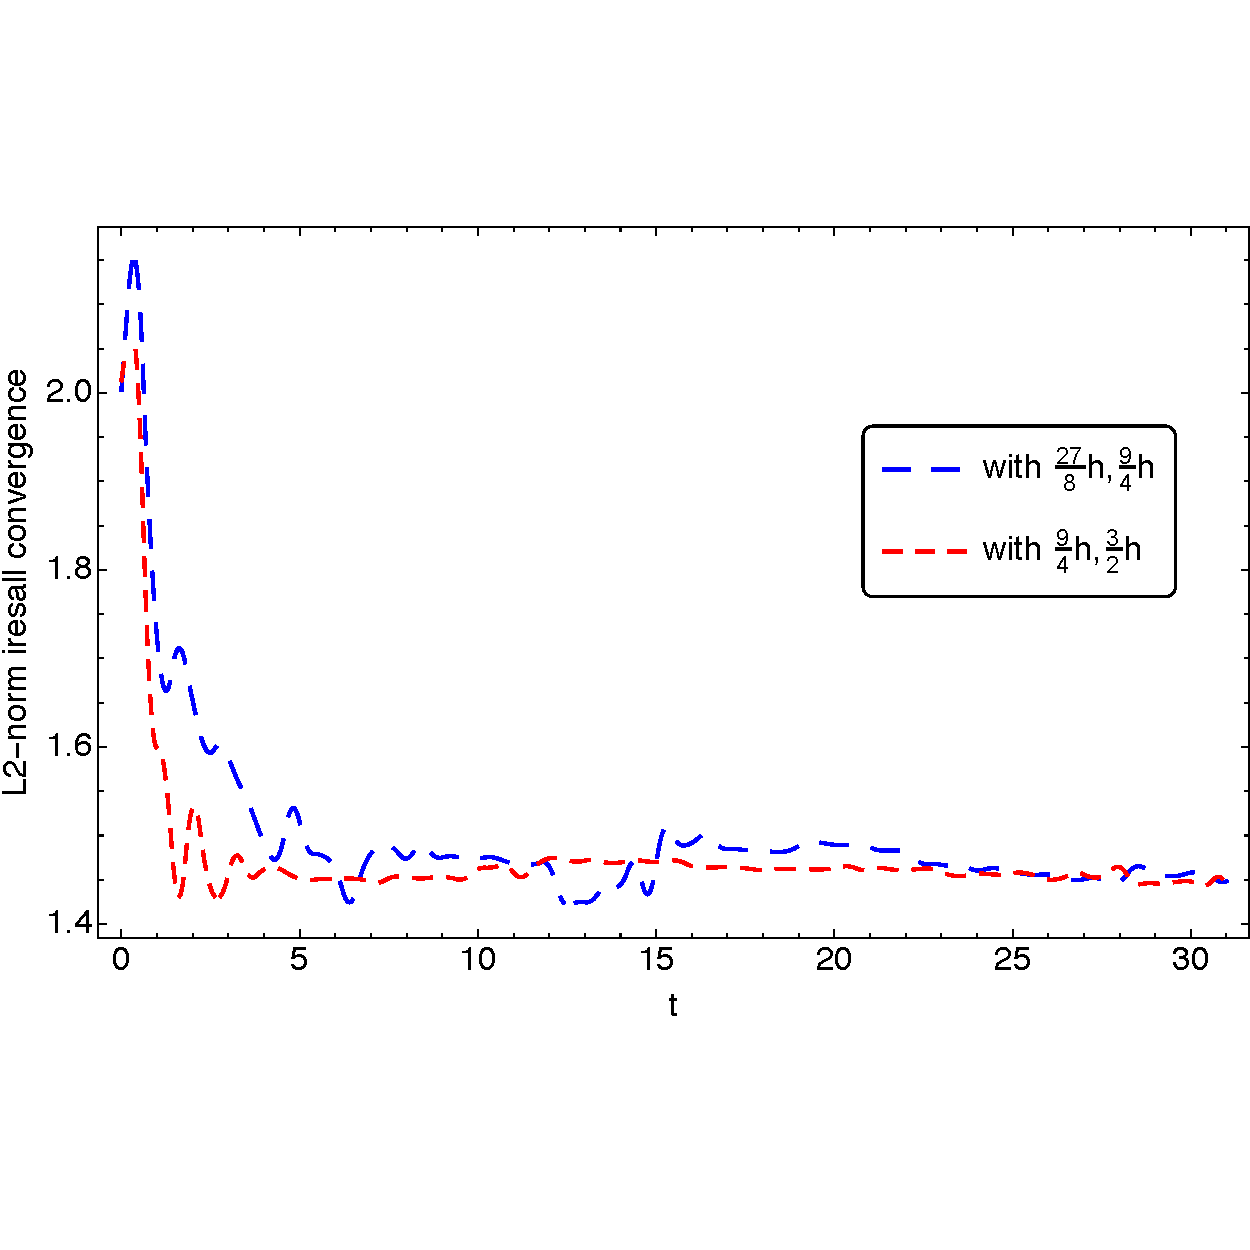
\includegraphics[width=5.0in,clip=true]{plots/timeseries/L2norm_iresallconvergence/fullplottL2normdim2boundedrescaledconvergenceiresallallres.pdf}
\parbox{5.0in}{\caption{Time evolution for $L^2$ norm of convergence factor for independent residual of Einstein equations at different resolutions.
        }\label{fig:L2norm_iresallconvergence-crop}}
\end{figure}

Figure \ref{fig:L2norm_iresallconvergence-crop} shows the $L^2$-norm of the convergence factor \eqref{eq:qires} for two pairs of resolutions. It clearly shows second order convergence to a solution of the Einstein equations, after an initial transition phase. However, the $L^2$-norm hides the fact that the order of convergence is lower (between 1 and 2) near the AdS boundary due to the use of first order interpolation, through which we impose the Dirichlet boundary conditions (see~\ref{subsec:cartevvarboucon}). More precisely, near-boundary convergence is higher for the lowest pair of resolutions than for the highest one, which shows values closer to 1 (as expected for first order interpolation). This is the reason why the $L^2$-norm of the lowest pair is largest.

\section{Extrapolation Technique and Convergence at AdS Boundary}\label{sec:extrapconvbdy}

As explained in Section~\ref{sec:bouset2}, given a Cartesian grid with spacing $\Delta$, since the AdS boundary generally does not lie on points of the grid, we can only obtain the approximated value $f^{bdy}_{\Delta}$ of any boundary quantity $f$ through extrapolation, using the numerical values of $f$ on grid points near the boundary, which we denote by $f_\Delta$. In this section we describe how grid points are chosen for extrapolation%and we show convergence for the extrapolation scheme by computing the factor \eqref{eq:qconv} for $f^{bdy}_{\Delta}$ at boundary points, which is expected as a consequence of bulk convergence (see~\ref{sec:convbulk}) at the chosen points
. For simplicity, we consider first order extrapolation, i.e. we extrapolate using two grid points. The following can be generalized to higher extrapolation orders in a straightforward way.

If we wish to test convergence of $f^{bdy}_{\Delta}$ in the continuum limit $\Delta\rightarrow0$, two crucial criteria for the choice of grid points that are \emph{suitable} for extrapolation must be satisfied. We will now explain them with the help of Fig.~\ref{fig:lego_circle}, which shows an example of the result of the application of these criteria in the first quadrant of a $z=const.$ surface of the grid for first order extrapolation.
\begin{enumerate}
 \item \emph{Common points.} Consider the value of $f^{bdy}_{\Delta}$ at any boundary point $p_{bdy}$. If we obtain this by $1^{st}-$order extrapolation, $f^{bdy}_{\Delta}(p_{bdy})$ is a combination of the values $f_\Delta(p_1),f_\Delta(p_2)$ (where $p_1,p_2$ are the bulk points used for extrapolation) multiplied by factors that depend on the coordinates of $p_{bdy},p_1,p_2$. Therefore, we can write  $f^{bdy}_{\Delta}(p_{bdy})=f(p_{bdy})+c_{extr}(p_{bdy},p_1,p_2)+c_\Delta(p_1,p_2)\Delta^2$ where the first term is the true value of $f$ at $p_{bdy}$, the second term is the error due to the extrapolation approximation and the third term is the error coming from the numerical error in $f_\Delta$. From this we immediately see that the convergence factor \eqref{eq:qconv} at point $p_{bdy}$ can be expected to asymptote to 2 as $\Delta\rightarrow0$ only if the points $p_1,p_2$ are the same for all 3 resolutions involved.
 
\item \emph{Convergent range.} For each resolution, grid points with $\rho\geq 1-\Delta/2$ (points outside the dotted line in Fig.~\ref{fig:lego_circle}) are excised due to the fact that some quantities diverge at $\rho=1$, the value of functions at points with $1-3\Delta/2\leq \rho < 1-\Delta/2$ (points between the dotted line and the dashed line in Fig.~\ref{fig:lego_circle}) are set by using forward/backward stencils, and the value of functions at points with $1-5\Delta/2\leq \rho < 1-3\Delta/2$ (between the dashed line and the continuous thin blue line in Fig.~\ref{fig:lego_circle}) are set by using centred stencils which, however, use neighbouring points set by forward/backward stencils. For all these reasons, we can only expect convergence if we pick grid points with  $\rho<1-5\Delta/2$ (inside the continuous blue line in Fig.~\ref{fig:lego_circle}). However, in practice, we see that we need to restrict the choice of suitable points to those satisfying $\rho<1-9\Delta/2$ (inside the thick blue line) and $\max(x,y,z)>1-\frac{17}{2}\left(\frac{3}{2}\right)^{n_\Delta}\Delta$ (outside the black line), where $n_\Delta$ denotes the degree of the three resolutions used for convergence, $n_{9h/4}=0,n_{3h/2}=1,n_{h}=2$ (notice that $\left(\frac{3}{2}\right)^{n_\Delta}\Delta$ is a constant for all three resolutions), in order to avoid unphysical of non-converging values of boundary quantities.
 \end{enumerate}
Furthermore, among the points satisfying 1. and 2., we want the ones that are closest to the boundary in order for extrapolation to provide a more accurate approximation.

%If we wish to test convergence of $f^{bdy}_{\Delta}$ in the continuum limit $\Delta\rightarrow0$, there are two crucial criteria for the choice of grid points that are \emph{suitable} for extrapolation. We will now explain them with the help of Fig.~\ref{fig:lego_circle}, which shows an example of the result of the application of these criteria in the first quadrant of a $z=const.$ surface of the grid for first order extrapolation.
%\begin{enumerate}
% \item Consider the value of $f^{bdy}_{\Delta}$ at any boundary point $p_{bdy}$. If we obtain this by $n^{th}-$order extrapolation, $f^{bdy}_{\Delta}(p_{bdy})$ is a combination of the values $f_\Delta(p_1),f_\Delta(p_2),\dots,f_\Delta(p_{n+1})$ (where $p_1,p_2,\dots,p_{n+1}$ are the bulk points used for extrapolation) multiplied by factors that depend on the coordinates of $p_{bdy},p_1,\dots,p_{n_{\Delta}+1}$. Theqrefore, we can write  $f^{bdy}_{\Delta}(p_{bdy})=f(p_{bdy})+c_{extr}(p_{bdy},p_1,p_2,\dots,p_{n+1})+c_\Delta(p_1,p_2,\dots,p_{n+1})\Delta^2$ where the first term is the true value of $f$ at $p_{bdy}$, the second term is the error due to the extrapolation approximation and the third term is the error coming from the numerical error in $f_\Delta$. From this we immediately see that the convergence factor \eqref{eq:qconv} at point $p_{bdy}$ can be expected to asymptote to 2 as $\Delta\rightarrow0$ only if the points $p_1,p_2,\dots,p_{n+1}$ are the same for all 3 resolutions involved.
 
 %\item For each resolution, grid points with $\rho\geq 1-\Delta/2$ (points outside the dotted line in Fig.~\ref{fig:lego_circle}) are excised due to the fact that some quantities diverge at $\rho=1$, the value of functions at points with $1-3\Delta/2\leq \rho < 1-\Delta/2$ (points between the dotted line and the dashed line in Fig.~\ref{fig:lego_circle}) are set by using forward/backward stencils, and the value of functions at points with $1-5\Delta/2\leq \rho < 1-3\Delta/2$ (between the dashed line and the continuous blue line in Fig.~\ref{fig:lego_circle}) are set by using centred stencils which, however, use neighbouring points set by forward/backward stencils. For all these reasons, we can only expect convergence if we pick grid points with  $\rho<1-5\Delta/2$ (inside the continuous blue line in Fig.~\ref{fig:lego_circle}).
 %\end{enumerate}
%Furthermore, among the points satisfying (i) and (ii), we want the ones that are closest to the boundary in order for extrapolation to provide a more accurate approximation.

\begin{figure}[h]
        \centering
        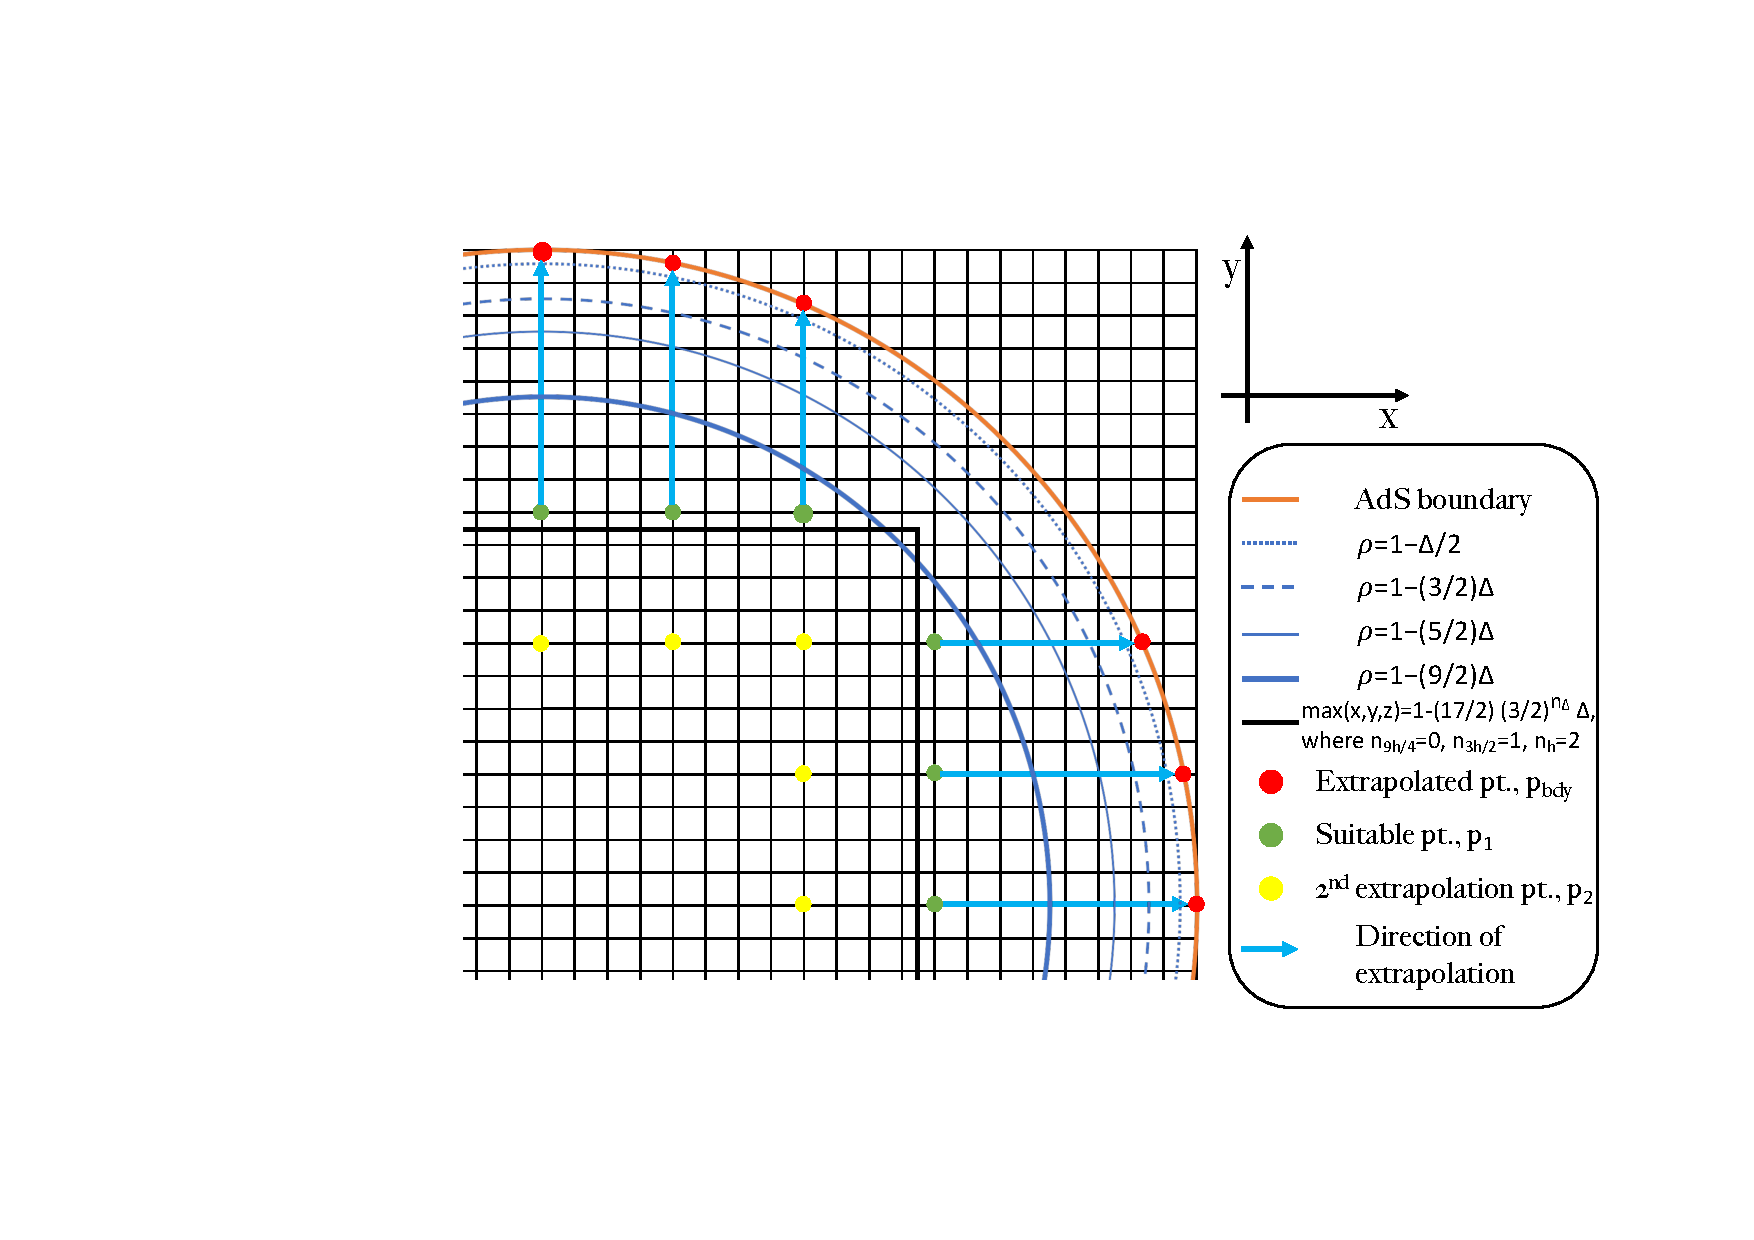
\includegraphics[width=5.0in,clip=true]{plots/lego_circle/Lego_circle_new.pdf}
\parbox{5.0in}{\caption{Visual description of first order extrapolation technique in the first quadrant of a $z=const.$ surface for the lowest resolution, with grid spacing $\Delta$, among the three involved in a convergence test ($const.$ is chosen as the $z-$coordinate value of one of the points common to all three resolutions). We show a typical example in which common points are 4 grid points away from each other along each direction.
        }\label{fig:lego_circle}}
\end{figure}
 
Once suitable points have been found (the green dots in Fig.~\ref{fig:lego_circle}), the extrapolation technique proceeds as follows:
 \begin{itemize}
 \item consider the first suitable point, $p_1$, and identify the coordinate with the largest value, e.g. $x$, and its sign, e.g. $x>0$. If two coordinates have the same value, then we pick $x$ over $y$ or $z$ and $y$ over $z$.
 \item take the next point, $p_2$, used for $1^{st}-$order extrapolation along the identified axis ($x$ in our example) in the direction of the bulk (decreasing $x$ in the example), making sure that they also satisfy 1. (2. is trivially satisfied by construction). Each $p_2$ is represented in yellow in Fig.~\ref{fig:lego_circle}.
 \item use $1^{st}-$ order extrapolation on $f_\Delta(p_1),f_\Delta(p_{2})$ to determine the value of $f^{bdy}_{\Delta}(p_{bdy})$ where $p_{bdy}$ is the boundary point along the identified axis in the direction of the boundary (one of the red dots in Fig. ~\ref{fig:lego_circle}). In our example, $p_{bdy}$ is the point with coordinates $(x,y,z)=(\sqrt{1-y(p_1)^2-z(p_1)^2},y(p_1),z(p_1))$.
 \item repeat the previous steps until the last suitable point.
 \end{itemize}

CONVERGENCE PLOTS

This extrapolation scheme is validated by Figure [CONVERGENCE], which shows second-order convergence at the boundary for CHOSEN FUNCTION with this extrapolation scheme, as expected from having second-order convergence in the bulk (see ~\ref{sec:convbulk}) at all points used for extrapolation.

Notice, from the discussion in (i), that we do not expect to converge to the true value $f(p_{bdy})$ of a boundary quantity in the continuum limit $\Delta\rightarrow0$, but rather to its approximation $f(p_{bdy})+c_{extr}(p_{bdy},p_1,p_2)$.
For this reason, the convergence test \eqref{eq:qires} cannot be performed at the boundary for functions with true value 0 (such as $\langle trT \rangle_{CFT}$), because their extrapolated value is not just the term linear in $\Delta^2$ but it also includes the extrapolation error $c_{extr}$.

Once convergence shows satisfactory trends for this extrapolation algorithm, we can relax the ``common points'' requirement 1., i.e. we can extrapolate from suitable points (selected within the convergent range discussed in 2.) and their neighbours in the direction of the bulk without requiring that all the points used are common to all resolutions. %Let us call this a \emph{free points} extrapolation scheme. 
This is the method we use for the boundary plots in Section~\ref{sec:resbouset} as it allows to extrapolate from points closer to the AdS boundary, thus giving a better approximation (i.e. a smaller extrapolation error, $c_{extr}$). Furthermore, for those plots we employ third order extrapolation (which employs four bulk points) since this improves the accuracy of the extrapolated numerical values even more, as tested by comparing with analytic predictions.

% Bibliography
%-------------------------------------------------------
\section*{References}
\bibliographystyle{JHEP}
\bibliography{3p1}


\end{document}

